\documentclass{article}
\usepackage[utf8]{inputenc}

\usepackage{eurosym} % per il simbolo dell'euro

\usepackage{array} % questo pacchetto serve per poter modificare le dimensioni delle colonne nella tabella così: m{numero em}.

\usepackage{graphicx} % per gli ambienti figure


\usepackage{amsmath} %per equation*


\usepackage{amssymb} %per mathbb


\usepackage{pgfplots}
\usepgfplotslibrary{fillbetween}



\title{Ricerca Operativa}
\author{Simone Palumbo}
\date{September 2021}

\begin{document}

\maketitle

\newpage

\section{Introduzione}
Il professore fa ricevimento quando volete. Sulle dispense c'è tutto e di più di quello che serve per preparare l'esame, oltre che tanti esercizi. Oltre a quello c'è anche un pdf con degli esercizi svolti.

\subsection{Perchè si chiama Ricerca Operativa?} 
Deriva dalla traduzione fatta male di un termine inglese "ricerca sulle operazioni" Operational Reseatch. In realtà si tratta di un corso di matematica applicata, una volta c'era un corso chiamato analisi numerica: questo è un corso di analisi numerica + qualcos'altro. Abbiamo detto che parleremo di matematica applicata: Analisi e Geometria, per esempio, sono effettivamente astratte, mentre R.O. applica queste due per risolvere problemi di decisione. Cioè problemi che riguardano una scelta. Entriamo subito nel vivo della materia con degli esempi.

\section{Problema di Produzione} 
Ovviamente semplificato rispetto alla realtà. Un colorificio produce 2 tipi di coloranti C1 C2 utilizzando 3 preparati P1 P2 P3. Sia C1 sia C2 usano P1 P2 P3 con diverse quantità quindi. La tabella seguente:
\begin{table}[h!]
    \centering
    \begin{tabular}{|m{5em}|m{2em}|m{2em}|m{6.5em}|}
    \hline
    hg/$\ell$ & C1 & C2 & q. max (hg/m)\\
    \hline
    P1 & 1 & 1 & 750\\
    \hline
    P2 & 1 & 2 & 1000\\
    \hline
    P3 & - & 1 & 400\\
    \hline
    \end{tabular}
    \vskip 0 pt
    \raggedright
    \hspace{2.345cm}
    \begin{tabular}{|m{5em}|m{2em}|m{2em}|}
    \hline
    Prezzo \euro/$\ell$ & 7 & 10\\
    \hline
    \end{tabular}
\end{table}
Riporta:
\begin{itemize}
    \item Le quantità (in ettogrammi\footnote{Questa cosa va ricordata per l'esame: \textit{le unità di misura contano!}}) di preparati base $P_i$ necessari per produrre un litro di colorante $C_i$
    \item Le disponibilità massime\footnote{In effetti la R.O. affronta il problema della limitatezza delle risorse.} (in ettogrammi al mese) di preparati base $P_i$
    \item Il prezzo di vendita (in euro al litro) dei due coloranti. Quindi da C2 guadagno di più ma consumo più risorse
\end{itemize}
Determinare la strategia ottima di produzione mensile.

\subparagraph{Risposta:} Dobbiamo scegliere quanto produrre di C1 e C2, almeno diverso da 0 perché devo fare soldi, voglio massimizzare quanto ricavo. Non posso scegliere arbitrariamente quanto produrre perché ho delle quantità limitate di risorse. Per prima cosa, essendo che siamo ingegneri, cerchiamo di scrivere in forma matematica la tabella, utilizzando delle incognite e usando disuguaglianze. Le incognite già ci immaginiamo quali possono essere: le quantità che dobbiamo produrre sono le incognite, e il profitto sarà incognite per costo. Ecco le due incognite:
\begin{itemize}
    \item $x_1$ indica la quantità di colori C1 in litri prodotta ogni mese. $x_1$ $\equiv q.$ tà in $\ell$/m di C1
    \item $x_2$ indica la quantità di colori C2 in litri prodotta ogni mese. $x_2$ $\equiv$ q. tà in $\ell$/m di C2
\end{itemize}
Quanto ricaviamo dalla vendita di C1 e C2 è quindi una funzione di $x_1$ e $x_2$:
\begin{itemize}
    \item dalla vendita di $x_1$ ricavo 7$x_1$ euro/m
    \item dalla vendita di $x_2$ ricavo 10$x_2$ euro/m
\end{itemize}
Quindi la funzione di ricavo totale:
\begin{equation*}
    p(x_1, x_2) = 7x_1 + 10x_2
\end{equation*}
Tra l'altro stiamo immaginando che tutto ciò che produciamo riusciamo a venderlo (ma è un'altra idealizzazione). Bene, il nostro obiettivo è determinare la strategia ottima di produzione, cioè vogliamo massimizzare i ricavi e cioè vogliamo massimizzare questa funzione, ricordandoci però che si hanno risorse limitate, cioè $x_1$ e $x_2$ possono prendere dei valori solo da 0 a una quantità che coincide con il totale dei preparati in magazzino utilizzati. Andiamo allora a vedere che quantità ci servono di questi preparati che abbiamo in magazzino:
\begin{itemize}
    \item P1: del primo preparato ne usiamo 1 etto per un litro di C1 e 1 etto per un litro di C2. Inoltre in magazzino ne abbiamo massimo 750 hg al mese. Quindi:
    \begin{equation*}
        P1_{usato} = 1 \cdot x_1 + 1 \cdot x_2 \leq 750
    \end{equation*}
    \item P2: del secondo preparato ne usiamo 1 etto per un litro di C1 e 2 etti per un litro di C2. Inoltre in magazzino ne abbiamo massimo 1000 hg al mese. Quindi:
    \begin{equation*}
        P2_{usato} = 1 \cdot x_1 + 2 \cdot x_2 \leq 1000
    \end{equation*}
    \item P3: del terzo preparato ne usiamo 1 etto per un litro di C2. Inoltre in magazzino ne abbiamo massimo 400 hg al mese. Quindi:
    \begin{equation*}
        P3_{usato} = 1 \cdot x_2 \leq 400
    \end{equation*}
\end{itemize}
Altra disuguaglianza importante, che potrebbe sembrare scontata ma ai fini degli esercizi è fondamentale, è che le quantità non possono essere negative, cioè:
\begin{equation*}
    x_1 \geq 0 \hspace{2cm} x_2 \geq 0
\end{equation*}
Bene, quindi abbiamo tradotto la tabella in un problema matematico di decisione, formato da incognite e disequazioni. Ora il nostro obiettivo è massimizzare i guadagni, cioè dobbiamo determinare $x_1$ e $x_1$ in modo che sia massimo il valore della funzione ricavo p($x_1,x_2$) = 7$x_1$ + 10$x_2$, rispettando però le disuguaglianze che abbiamo, che derivano dal fatto che le risorse sono limitate. Ora entriamo nel campo della geometria analitica: le produzioni $x_1$ e $x_1$ sono punti nel piano cartesiano, ma alcune di queste coppie di punti non sono ammissibili, perché non rispettano le disuguaglianze di sopra. Ora, per risolvere il problema, vogliamo disegnare sul piano cartesiano la regione dei punti che soddisfa queste disuguaglianze. Considerando già che $x_1 \geq 0$ e $x_2 \geq 0$, iniziamo con la disuguaglianza $x_1 + x_2 \leq 750$:
\begin{figure}[h!]
    \centering
    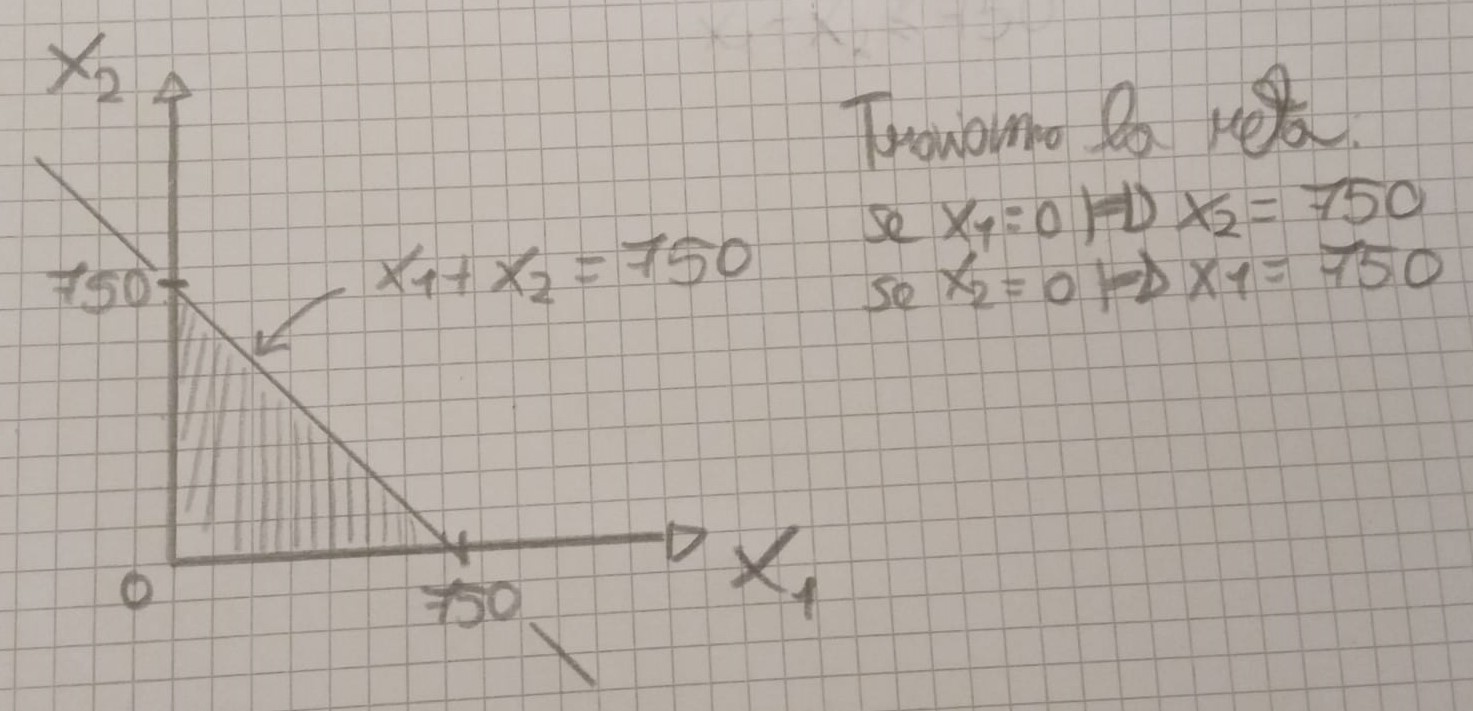
\includegraphics[scale=0.3]{retta1.jpeg}
\end{figure}
Quindi prima si trova la retta, dopodiché si trova la regione di spazio, tra le due sezionate dalla retta, i cui punti rispettano la disuguaglianza, e la si colora. Per fare quest'ultima cosa ci sono due modi:
\begin{itemize}
    \item Si prende un punto qualsiasi in una delle due regioni e si vede se la disuguaglianza, calcolata nei valori di quel punto, è rispettata, in tal caso la regione ammissibile è proprio quella a cui appartiene il punto, al contrario se la disuguaglianza non è rispettata la regione ammissibile è l'altra
    \item Valido solo se c'è vincolo di maggiore uguale. Si prendono i coeffficienti che moltiplicano le incognite, nel nostro caso 1 e 1 che moltiplicano rispettivamente $x_1$ e $x_2$. Si disegna il vettore che ha come componenti questi coefficienti, questo vettore punta alla regione ammissibile. Questo perché i vettori costruiti così sono ortogonali rispetto alla retta da cui sono stati costruiti, quindi possono assumere solo due versi. Il vettore quindi ha solo due zone a cui puntare, e quella a cui effettivamente punta è la zona ammissibile. Nota che se i coefficienti che fanno da componenti del vettore sono troppo grandi o troppo piccoli, puoi moltiplicare o dividere entrambe le componenti per lo stesso scalare positivo, in modo da preservare il verso del vettore e averne uno più comodo. Se c'è vincolo di minore uguale allora devi prendere la zona NON puntata dal vettore come zona ammissibile.
\end{itemize}
Ripetiamo lo stesso procedimento per le due disuguaglianze rimaste:
\begin{figure}[h!]
    \centering
    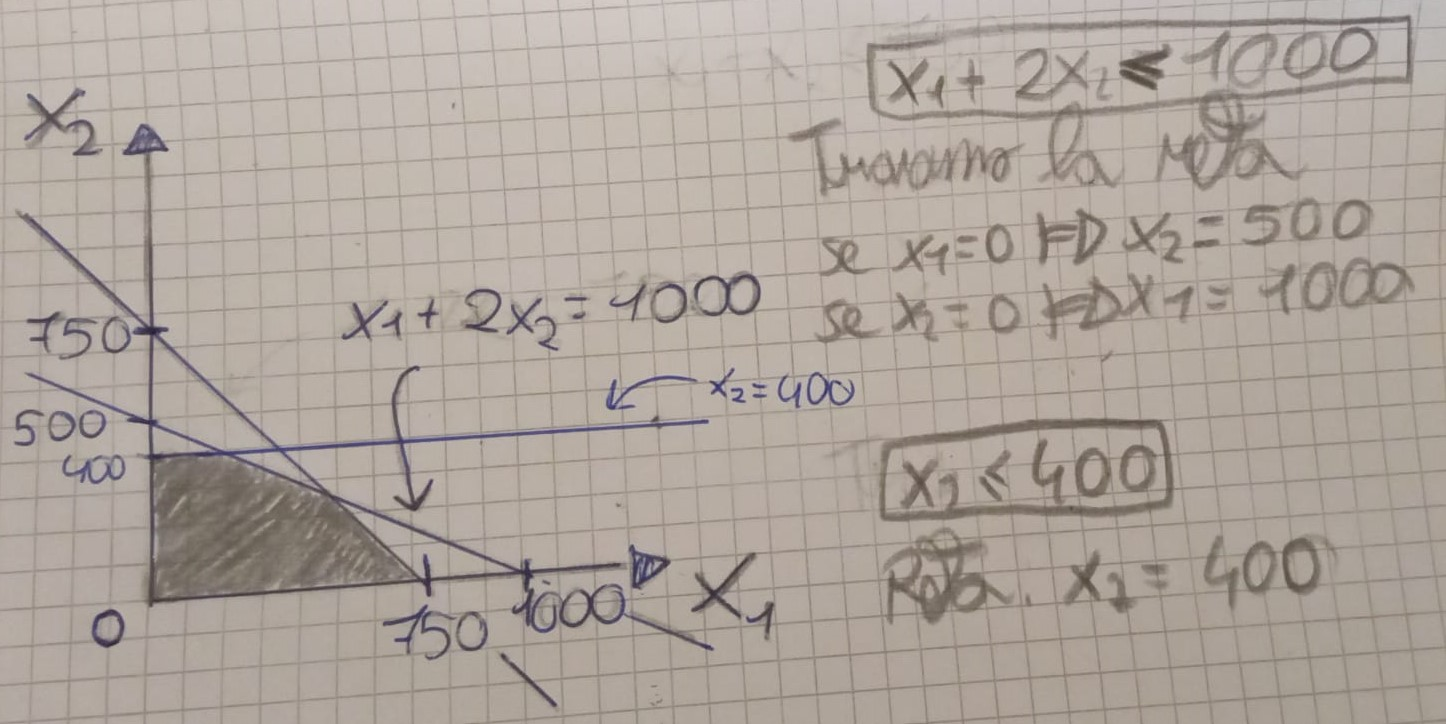
\includegraphics[scale=0.3]{retta2}
\end{figure}
Adesso sappiamo la porzione di piano dei punti ammissibili, ma ci manca ancora un passaggio importante: calcolare le intersezioni tra le rette. Ovviamente consideriamo i punti di intersezione che cadono nella zona ammissibile, poichè le intersezioni in una zona non ammissibile non ci interessano. Quindi, calcolando tutte le possibili intersezioni tramite tutti i sistemi di equazioni necessari troviamo:
\begin{figure}[h!]
    \centering
    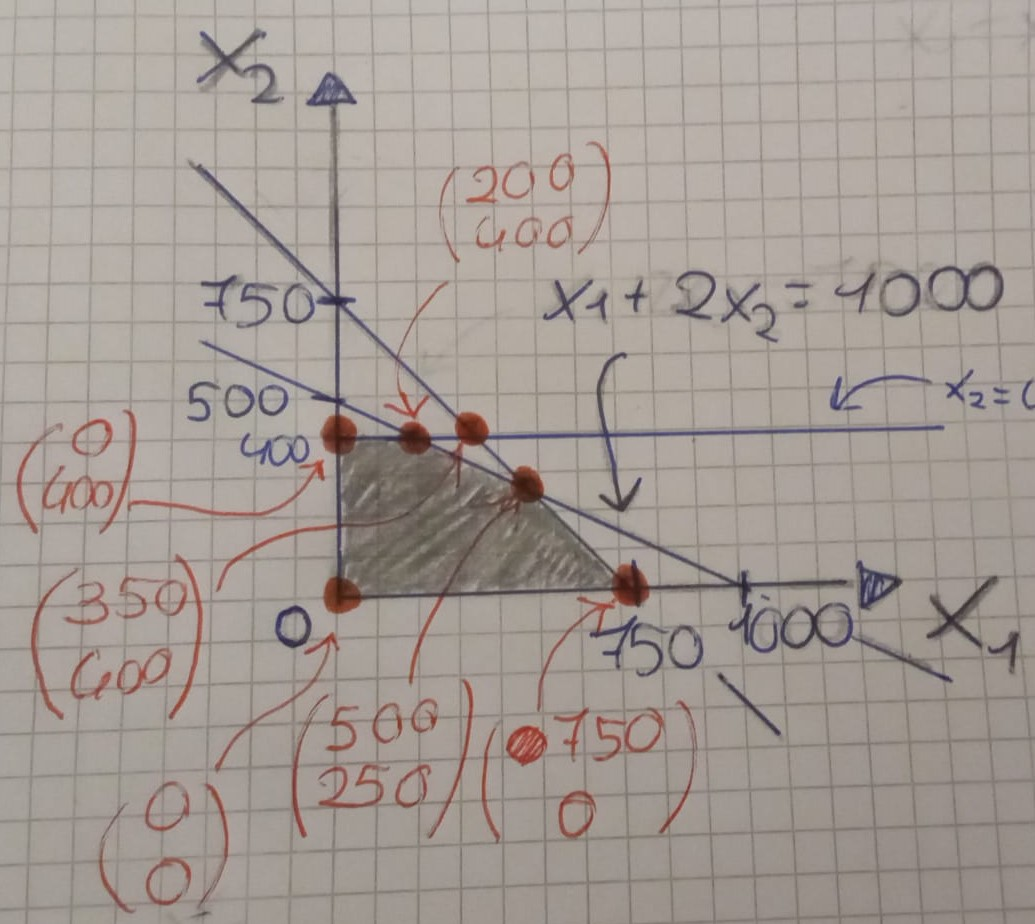
\includegraphics[scale=0.3]{retta3.jpeg}
\end{figure}
Vediamo che il punto di intersezione $\binom{350}{400}$ non ci interessa, perché è fuori dalla zona ammissibile. Bene ora abbiamo tutto ciò che ci serve per far entrare in campo la funzione ricavo. In effetti per ora abbiamo soltanto trovato infiniti punti che sono ammissibili, ma noi vogliamo trovare il/i migliore/i, quello/i che ci fa/fanno massimizzare il guadagno. La funzione ricavo serve proprio a questo: ordina questi infiniti punti, permettendoci di prendere il più grande tra loro. Ora il discorso è semplice, prendiamo  $7x_1 + 10x_2$ indica infinite rette, e fissando un valore che questa funzione deve assumere fissiamo una retta. Più alto il valore che fissiamo, più guadagno abbiamo. Dobbiamo quindi trovare il valore più alto che possiamo far assumere alla funzione t.c. rientri nella zona ammissibile; $x_1$ e $x_2$ che realizzeranno questo valore fissato della funzione sono le nostre migliori scelte per la produzione. Iniziamo provando a fissare $7x_1 + 10x_2$ = 0:
\begin{figure}[h!]
    \centering
    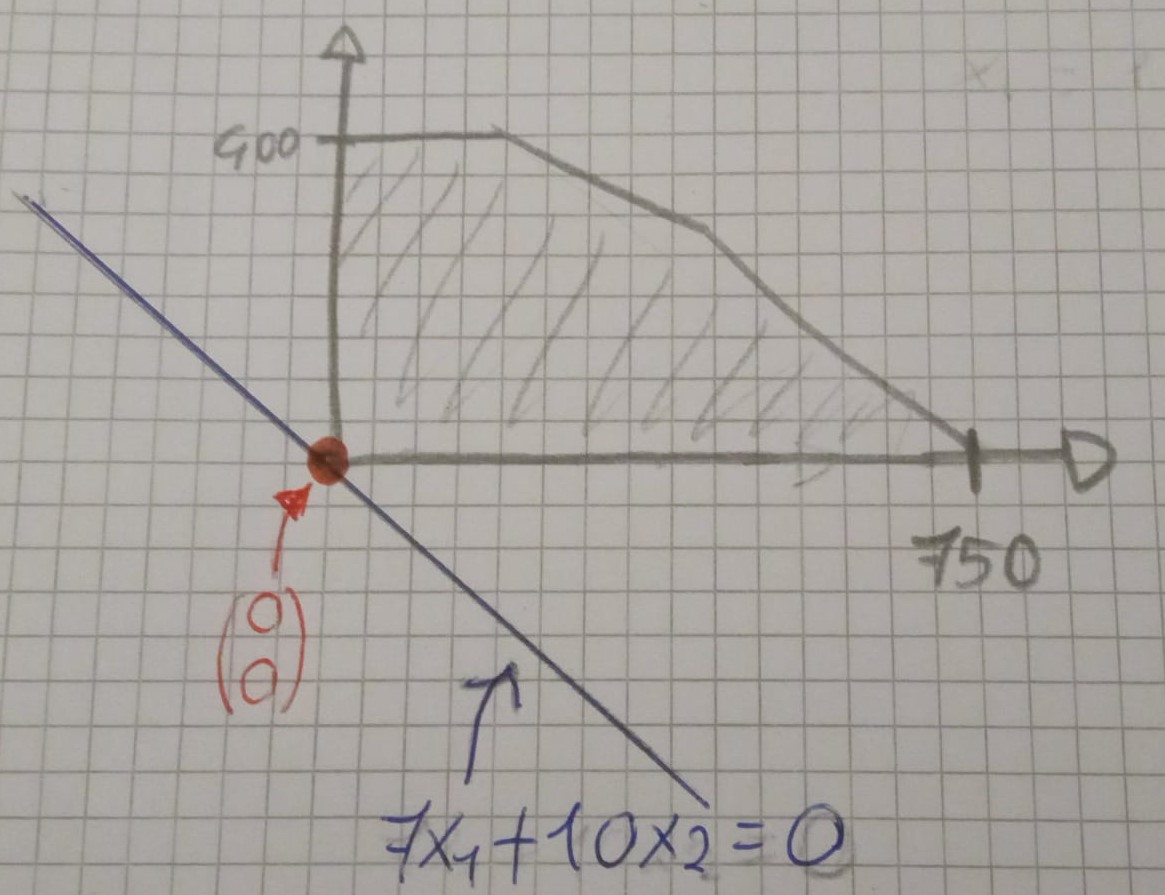
\includegraphics[scale=0.3]{rettaricavotot.jpeg}
\end{figure}

Vediamo che l'unico punto della retta che ricade in zona ammissibile è (0,0), ma non ci va bene perché non spendiamo nulla e non guadagniamo nulla. Quindi, sappiamo che alzando i valori che $7x_1 + 10x_2$ assume otteniamo sempre un guadagno maggiore, proviamo a trovare quel suo valore più alto per cui c'è almeno un punto nella zona ammissibile. Dato che abbiamo dei punti di intersezione lontani dall'origine, il ché significa che ci fa guadagnare di più, proviamo a calcolare il valore di $7x_1 + 10x_2$ in quei valori. Si vede, provandoli tutti, che nel punto di intersezione $\binom{500}{250}$ si ha il valore più alto di tutti, poiché ci fa guadagnare $7\cdot500 + 10\cdot250 = 6000$.
\begin{figure}[h!]
    \centering
    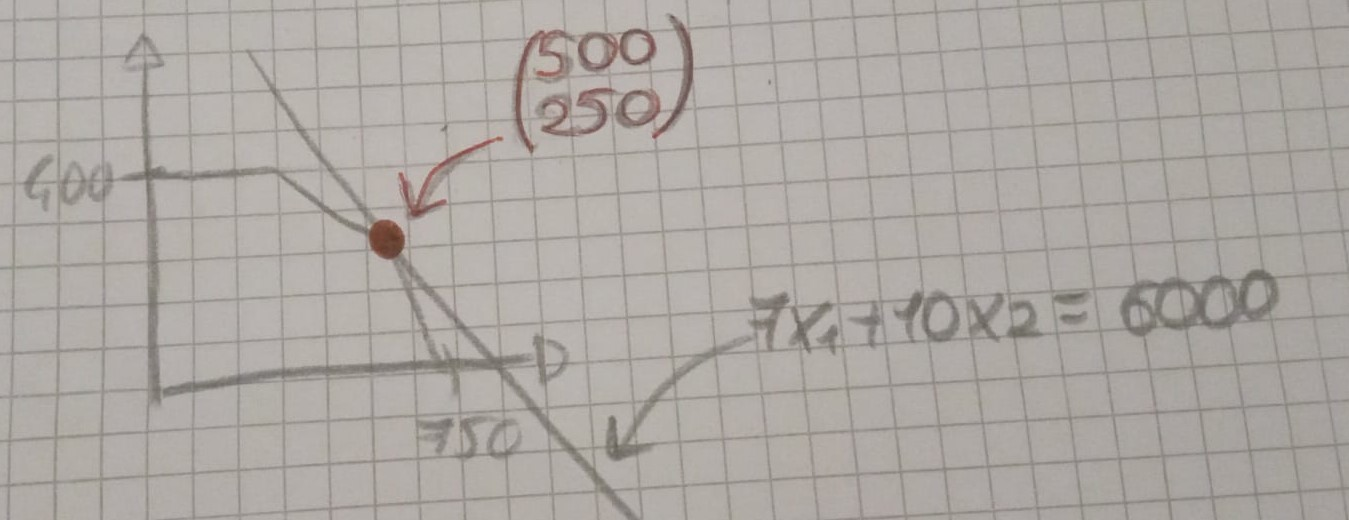
\includegraphics[scale=0.3]{rettaricavototfinale.jpeg}
\end{figure}
Quindi questo è il ricavo totale più alto che posso avere, prima di uscire dalla zona non ammissibile. Questo perché appena provo a mettere un termine noto appena appena più alto di 6000 la retta non ha più intersezioni con la zona ammissibile. Quindi con $x_1 = 500$ e $x_2 = 250$ ho massimizzato il profitto. Notare infine che il fatto che questa retta, di cui TUTTI i punti fanno guadagnare 6000, ha solo questo punto nella zona ammissibile, vuol dire che $x_1$ e $x_2$ che ci fanno guadagnare il massimo sono unici, non ci sono più possibilità per guadagnare il massimo. Quindi per risolvere i problemi: scriviamo il problema matematicamente (con incognite e disuguaglianze), poi, avendo due variabili, ho disegnato la zona ammissibile nel piano con le disuguaglianze e ho trovato il termine noto massimo che fa intersecare la funzione ricavo totale con la zona ammissibile.
 
\vspace{1cm}

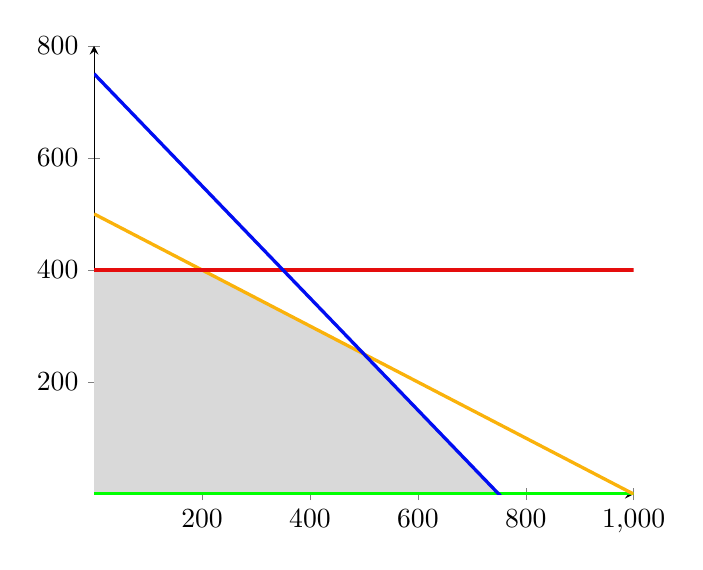
\begin{tikzpicture}
  \begin{axis}[
    axis lines=middle,
    xmin=0, xmax=1000,ymin=0,ymax=800
  ]
  \addplot[very thick,green, samples=300, domain=0:1000, name path=A] {0}; 
  \addplot[very thick,yellow!70!red, samples=300, domain=0:1000, name path=B] {(1000-x)/2}; 
  \addplot[very thick,red!90!teal, samples=300, domain=0:1000, name path=C] {400}; 
  \addplot[very thick,blue!90!teal, samples=300, domain=0:1000, name path=D] {750-x}; 
  \addplot[gray!30] fill between[of=A and C,soft clip={domain=0:200}];
  \addplot[gray!30] fill between[of=A and B,soft clip={domain=199:500}];
  \addplot[gray!30] fill between[of=A and D,soft clip={domain=499:750}];
  \end{axis}
\end{tikzpicture}


%PUOI PROVARE A USARE QUESTO TRICK DI SOFT CLIP PER COLLEGARE TRA LORO LE AREE https://tex.stackexchange.com/questions/344021/pgfplots-fillbetween-with-multiple-curves

\vspace{1cm}


\section{Sette Lunedì:}
La ricerca operativa entra in una storia di montalbano. C'è un episodio che si chiama sette lunedì. Nell'episodio montalbano pretende di risolvere uno dei problemi più difficili della ricerca operativa. Lui traccia su uno stradario tutti i punti in cui c'è una casa dove devono andare, e chiede al suo aiutante di tracciare il percorso più breve che contempli tutti questi punti così da avvisare tutti nel minor tempo possibile. Si chiama problema del commesso viaggiatore. 


\section{Problema di Ottimizzazione:} In matematica e in informatica, un problema di ottimizzazione è il problema di trovare la migliore soluzione fra tutte le soluzioni fattibili. Sia f: $\mathbb{R}^n \to \mathbb{R}$ e sia S $\subseteq \mathbb{R}^n$; si definisce \textit{problema di ottimizzazione} un problema formulato nel seguente modo: determinare
\begin{equation*}
    min f(x)
\end{equation*}
sapendo
\begin{equation*}
    x \in S 
\end{equation*}
Oppure nel seguente modo: determinare 
\begin{equation*}
    max f(x)
\end{equation*}
sapendo
\begin{equation*}
    x \in S 
\end{equation*}
Chiamiamo \textit{f} funzione obiettivo e S \textit{l'insieme ammissibile}. Se abbiamo un problema di ottimizzazione, abbiamo allora che:
\begin{itemize}
    \item Il problema si dice inammissibile se S = $\varnothing$
    \item Il problema si dice illimitato inferiormente quando, per ogni M $>$ 0 è possibile trovare una x $\in$ S t.c. f(x) $<$ -M, e si dice illimitato superiormente quando, per ogni M $>$ 0 è possibile trovare una x $\in$ S t.c. f(x) $>$ M
    \item Nel caso in cui si debba determinare il minimo di f(x) il problema ammette soluzione ottima se $\exists x^* \in S$ t.c. f(x$^*$) $\leq$ f(x), $\forall x \in S$. In questo caso chiamiamo $x^*$ minimo globale o soluzione ottima e f(x$^*$) il valore ottimo. Nel caso in cui si debba determinare il massimo di f(x) il problema ammette soluzione ottima se $\exists x^* \in S$ t.c. f(x$^*$) $\geq$ f(x), $\forall x \in S$. Anche in questo caso chiamiamo $x^*$ soluzione ottima e f(x$^*$) il valore della soluzione ottima.
\end{itemize}
Nella trattazione teorica dei problemi di ottimizzazione, per semplicità, decidiamo di scrivere in una sola forma tra min e max. \textit{Per convenzione scegliamo min}:
\begin{equation*}
    min f(x)
\end{equation*}
Anche perché passare dall'una all'altra forma è facilissimo, basta ricordarsi che trovare il min di f(x) equivale a trovare il max di - f(x). Quindi si può passare da un problema di minimo a uno di massimo semplicemente cambiando la funzione.



\subsection{Classificazione dei Problemi:} 
\begin{itemize}
    \item Ottimizzazione continua: quando le variabili possono assumere valori reali
    \begin{itemize}
        \item vincolata quando S $\subset \mathbb{R}^n$
        \item non vincolata quando S = $\mathbb{R}^n$
    \end{itemize}
    \item Ottimizzazione discreta: quando le variabili possono assumere valori interi
    \begin{itemize}
        \item programmazione a numeri interi quando S $\subset \mathbb{Z}^n$
        \item programmazione combinatoria (o programmazione 0/1, o programmazione binaria) quando S $\subseteq \{0,1\}^n$. Molti problemi sono di questo tipo.
        \item programmazione mista-intera quando solo alcune variabili devono assumere valori interi
    \end{itemize}
\end{itemize}
Ora parliamo dell'insieme ammissibile S, esso \underline{solitamente} è descritto da un sistema finito di disuguaglianze del tipo g(x) $\geq$ b (o anche uguaglianze, essendo un'uguaglianza una coppia di disuguaglianze), che chiamiamo \textit{vincoli}, con g(x): $\mathbb{R}^n$ $\to$ $\mathbb{R}$. Cioè:
\begin{equation*}
    S = \{x \in \mathbb{R}^n: g_1(x) \geq b_1, ..., g_m(x) \geq b_m\}
\end{equation*}
Diciamo che, dato un punto $\bar{x}$, un vincolo $g_i(\bar{x}) \geq b_i$ è:
\begin{itemize}
    \item Soddisfatto in $\bar{x}$ quando $g_i(\bar{x}) \geq b_i$ è vera. Un caso particolare è il vincolo attivo, cioè $\bar{x}$ quando $g_i(\bar{x}) = b_i$. Qui il vincolo è soddisfatto ma all'uguaglianza.
    \item Violato in $\bar{x}$ quando $g_i(\bar{x}) \geq b_i$ è falsa
    \item Ridondante quando la sua eliminazione non muta l'insieme ammissibile. Questo non ha nulla a che fare con la soddisfazione o meno del vincolo: un vincolo ridondante può essere anche un vincolo vietato.
\end{itemize}
Quindi, ricapitolando in un problema di ottimizzazione di questo tipo, abbiamo una funzione obiettivo che vogliamo ottimizzare, ad esempio minimizzare:
\begin{equation*}
    min f(x)
\end{equation*}
E m disuguaglianze da rispettare:
\begin{equation*}
    s.t. \hspace{0.2cm} g_i(x) \geq b \hspace{1.5cm} i = 1, ..., m
\end{equation*}
Quando ciò avviene si parla di un problema di Programmazione Matematica. Precisamente si parla di:
\begin{itemize}
    \item Programmazione Matematica Lineare (PL): quando f(x) e tutte le $g_i(x)$ sono lineari
    \item Programmazione Matematica NonLineare (PNL): quando almeno una tra $g_i(x)$ oppure f(x) sono una funzione nonlineare.
\end{itemize}


\paragraph{Facciamo un esempio:} 
\begin{equation*}
    min f(x) = min 3x_1 + x_2
\end{equation*}
Con $3x_1 + x_2$ funzione obiettivo.
\begin{equation*}
    \begin{cases}
        \text{$x_1^2 + x_2^2 \leq 4$}\\
        \text{$x_1 \geq 0$} 
    \end{cases}
\end{equation*}
Sono i nostri vincoli. Che possiamo scrivere nella forma dell'insieme ammissibile in questo modo:
\begin{equation*}
    S = \{x \in \mathbb{R}^2: x_1^2 + x_2^2 \leq 4, x_1 \geq 0\}
\end{equation*}
Bene, classificare il problema. Allora vediamo, abbiamo un insieme ammissibile definito solo attraverso diseguaglianze, e dobbiamo trovare il minimo di una funzione: siamo di fronte a un problema di Programmazione Matematica. Inoltre vediamo che anche se f(x) è lineare, il primo vincolo presenta una funzione non lineare, quindi è una PLN.

\paragraph{E questo esempio?} 
\begin{equation*}
    min 3x_1 + 4x_1 
\end{equation*}
Con vincoli:
\begin{equation*}
\begin{cases}
    \text{$log(2)x_1 + sin(\pi/3)x_2 \geq 7$}\\
    \text{$x_2 \leq 0$}
\end{cases}
\end{equation*}
Questo è un PL: infatti la funzione obiettivo è lineare, e - non facciamoci ingannare dai coefficienti - anche i vincoli lo sono.

\paragraph{Ultimo esempio...}
\begin{equation*}
    min sin(x_1) + 8x_2
\end{equation*}
Con vincolo:
\begin{equation*}
(x_1,x_2) \in S \Longleftrightarrow x_1 \hspace{0.2cm} \text{è un numero pari} \hspace{0.2cm} \lor \hspace{0.2cm} x_1 = 7^m,  m \in \mathbb{N}
\end{equation*}
Qua vediamo che i vincoli (che in questo caso è uno solo) che formano l'insieme ammissibile non sono tutte disuguaglianze, quindi questo non è un problema di Programmazione Matematica. Ma è comunque un problema di ottimizzazione. Il discorso è che noi, in questo corso, questi tipi di problemi non li considereremo, perché consideriamo solo quelli di Programmazione Matematica e, per la maggior parte del corso, esclusivamente i PL. Vediamo ora un esempio di Programmazione Matematica Binaria.

\subsection{Problema di Capital Budgeting, Programmazione Binaria:} 
Un piccoloinvestitore deve stabilire come investire il proprio capitale potendo
scegliere tra 6 dierenti investimenti. L'investitore dispone di un budget di
100000e e conosce i costi di attivazione nonché il Net Present Value (NPV)
di ciascuno di essi come riportato nella tabella che segue:
\begin{table}[h!]
    \centering
    \begin{tabular}{|c||c|c|}
    \hline
    & costo (in migliaia di \euro) & NPV\\
    \hline
    \hline
    inv.1 & 100 & 40\\
    \hline
    inv.2 & 50 & 35\\
    \hline
    inv.3 & 45 & 18\\
    \hline
    inv.4 & 20 & 4\\
    \hline
    inv.5 & 10 & 10\\
    \hline
    inv.6 & 5 & 2\\
    \hline
    \end{tabular}
\end{table}
Quali investimenti attivare per fare in modo che il NPV sia il più grande possibile? Questo è un problema particolare: mentre nel problema precedente dovevamo scegliere quanto produrre, e le soluzioni potevano essere frazionarie, qui le scelte che possiamo fare, per ogni investimento, sono solo 0 o 1 (investimento non attivo o attivo). Per problemi come questo o simili a questo è ragionevole introdurre queste variabili
\begin{equation*}
    x_i = 
    \begin{cases}
        \text{1 se l'investimento i è attivato}\\
        \text{0 altrimenti}
    \end{cases}
\end{equation*}
Quindi avrò un vettore di 6 variabili composto da 0 e 1. Questo viene chiamato \textit{Vettore di Incidenza}, ed è un vettore x $\in$ \{0,1\}$^6$. Quindi siamo di fronte a un problema di Programmazione Matematica binaria. Dato uno di questi vettori, possiamo calcolarci il costo totale degli investimenti scelti dal vettore, così: prendiamo la somma di tutti i costi moltiplicando ognuno di essi per la rispettiva variabile $x_i$. Se chiamiamo $c_i$ il costo (in migliaia di \euro) dell'i-esimo investimento, in formule questo è:
\begin{equation*}
    \sum_{i=1}^6 c_ix_i 
\end{equation*}
Questo ci da il costo totale relativo a un certo vettore di incidenza. Infatti, anche se io sto sommando tutti e 6 gli investimenti, quelli non attivati dal vettore scelto non compariranno nella somma, poiché il loro costo verrà moltiplicato per $x_i = 0$. Bene, ora noi sappiamo di avere un budget massimo di 100000 euro, quindi:
\begin{equation*}
    \sum_{i=1}^6 c_ix_i \leq 100000
\end{equation*}
Questa disuguaglianza definisce l'insieme S ammissibile, dicendoci quali vettori di incidenza sono ammissibili e quali no. Adesso andiamo a calcolare la funzione obiettivo: il NPV, che dobbiamo massimizzare. Utilizzando lo stesso ragionamento fatto prima per il costo totale, e chiamando $p_i$ il NPV relativo all'i-esimo investimento si ha che la funzione obbiettivo è:
\begin{equation*}
    \sum_{i=1}^6 p_ix_i 
\end{equation*}
Quindi il nostro problema è stato matematicizzato nel seguente modo:
\begin{equation*}
    max_x \sum_{i=1}^6 p_ix_i
\end{equation*}
Dove usiamo max perché questa funzione noi vogliamo massimizzarla, per guadagnare il più possibile.
\begin{equation*}
    s.t. \hspace{0.2cm} \sum_{i=1}^6 c_ix_i \leq 100000
\end{equation*}
Sapendo inoltre che è un problema di Programmazione binaria:
\begin{equation*}
    x \in \{0,1\}^6
\end{equation*}
Non ci interessa risolverlo, era solo per impostarlo.


\section{Problemi di PL:} 
Innanzitutto facciamo un richiamo:
\paragraph{Funzione Lineare:}
Funzione lineare: una funzione f: $\mathbb{R}^n \to \mathbb{R}$ si dice \textit{lineare} quando rispetta:
\begin{itemize}
    \item L'additività: $\forall x, y \in \mathbb{R}^n$ , f(x + y) = f(x) + f(y)
    \item La proporzionalità: $\forall x, y \in \mathbb{R}^n$ , $\lambda \in \mathbb{R}, f(\lambda x) = \lambda f(x)$
\end{itemize}
Questo ci porta a dedurre la proprietà per cui una funzione lineare si può sempre scrivere come somma di prodotti tra le componenti di una sua variabile e dei coefficienti, in formule:
\begin{equation*}
    f: \mathbb{R}^n \to \mathbb{R} \text{è lineare} \Longleftrightarrow \exists c_i, i = 1,..., n \text{t.c.} 
\end{equation*}
\begin{equation*}
    f(x) = c_1x_1 + .... + c_nx_n
\end{equation*}
Lo possiamo dedurre dicevamo dalle precedenti proprietà così: prendiamo una funzione f(x): $\mathbb{R}^n \to \mathbb{R}$ lineare. Prendiamo una variabile x $\in \mathbb{R}^n$. Essendo x un vettore di $\mathbb{R}^n$ Lo posso scrivere come combinazione lineare dei vettori della base canonica di $\mathbb{R}^n$
\begin{equation*}
    x = \sum_{i=1}^n x_ie_i
\end{equation*}
Con $x_i$ i-esima componente del vettore x e $e_i$ i-esimo vettore della base canonica. Quindi è la somma di prodotti tra uno scalare e un vettore. Bene ora applico la funzione lineare:
\begin{equation*}
    f(x) = f(\sum x_i e_i) = \sum f(x_i e_i) = \sum x_if(e_i)
\end{equation*}
Per la proprietà di additività e poi di proporzionalità. Adesso, sapendo che la funzione calcolata in un valore produce un altro valore, costante, in $\mathbb{R}$, chiamo questo valore c. Quindi $f(e_i) = c_i$ e abbiamo:
\begin{equation*}
    f(x) = \sum x_ic_i
\end{equation*}





\subsection{Forma matriciale del problema di PL:}
Scriviamo innanzitutto ciò che sappiamo del nostro problema:
\begin{equation*}
    min f(x) = min c_1 + x_1 + ... + c_n x_n 
\end{equation*}
E i vincoli:
\begin{equation*}
    \begin{cases}
        \text{$a_{11}x_1 + ... + a_{1n}x_n \geq b_1$}\\
        \text{$a_{21}x_1 + ... + a_{2n}x_n \geq b_2$}\\
        \text{...}\\
        \text{$a_{m1}x_1 + ... + a_{mn}x_n \geq b_m$}\\
    \end{cases}
\end{equation*}
Ora ci possiamo ricordare, dalla Geometria Analitica, che il \textit{prodotto scalare} tra due vettori è definito come la somma dei prodotti tra le corrispettive componenti dei due vettori, cioè:
\begin{equation*}
    a \cdot x = \sum_{i=1}^n a_ix_i
\end{equation*}
E, analogamente, possiamo ricordarci che il prodotto scalare di due vettori dà lo stesso risultato del prodotto matriciale tra il primo vettore trasposto e il secondo non trasposto, cioè:
\begin{equation*}
    a \cdot x = a^{T}x
\end{equation*}
In ogni caso, questo fa al caso nostro, poiché vediamo che ogni vincolo è proprio definito come la somma dei prodotti tra le componenti di a e quelle di x, quindi possiamo scrivere i vincoli come:
\begin{equation*}
    \begin{cases}
        \text{$a_1\cdot x = a_1^{T}x \geq b_1$}\\
        \text{$a_2\cdot x = a_2^{T}x \geq b_2$}\\
        \text{...}\\
        \text{$a_m\cdot x = a_m^{T}x \geq b_m$}\\
    \end{cases}
\end{equation*}
Ovviamente stessa cosa possiamo fare con la funzione obiettivo, scrivendo:
\begin{equation*}
    min \hspace{0.2cm} c \cdot x = min \hspace{0.2cm} c^{T}x
\end{equation*}
E, finalmente, compattamente la possiamo scrivere in forma matriciale:
\begin{equation*}
    Ax \geq b    
\end{equation*}
Con A matrice dei coefficienti con m righe e n colonne, x vettore delle incognite e b vettore dei termini noti.
Questa è la \textit{forma generale di un problema di PL}. Ma come la più generale? non presenta vincoli di uguaglianza ad esempio! Ma io una uguaglianza posso scriverla sempre come una coppia di disuguaglianze, quindi sì è la più generale.



\paragraph{Angolo tra vettori in $\mathbb{R}^n$} Anche questo è un richiamo. Siano x,y $\in \mathbb{R}^n$, $x,y \neq 0$, allora:
\begin{equation*}
    x \cdot y = x^{T}y = \sum_{i=1}^n x_iy_i = ||x|||y||cos\phi
\end{equation*}
Con $\phi$ l'angolo tra x e y. Vediamo che quando il prodotto scalare viene 0 il coseno è 0, quindi $\phi = \frac{\pi}{2}$, e quindi i due vettori sono ortogonali. Notare che i vettori della base canonica sono, a coppie, tutti ortogonali tra loro. Ma a che ci serve? Questo ci aiuta a stabilire una proprietà dell'equazione di una retta in $\mathbb{R}^2$, un piano in $\mathbb{R}^3$ o un iperpiano in $\mathbb{R}^n$. La proprietà è questa, prendiamo l'iperpiano in $\mathbb{R}^n$ di equazione $a^{T}x = b$, con $a \in \mathbb{R}^n$, $x \in \mathbb{R}^n$, e fissato $b \in \mathbb{R}$. Siano $\bar{x}$ e $\bar{y}$ due vettori \textit{distinti}, che soddisfano l'equazione, cioè che sono sull'iperpiano. Ciò vuol dire che soddisfano:
\begin{equation*}
    a^{T}\bar{x} = b \hspace{1cm} a^{T}\bar{y} = b
\end{equation*}
Adesso sottraiamo una all'altra e otteniamo:
\begin{equation*}
    a^{T}(\bar{y}-\bar{x})7 = 0
\end{equation*}
Che per quanto detto sul prodotto scalare, ci dice che il vettore a è ortogonale a $\bar{x}-\bar{y}$. Questo è valido in $\mathbb{R}^n$ come già detto, ma per fissare le idee vediamo in $\mathbb{R}^2$, dove l'equazione descrive una retta, cosa significa:
\begin{figure}[h!]
    \centering
    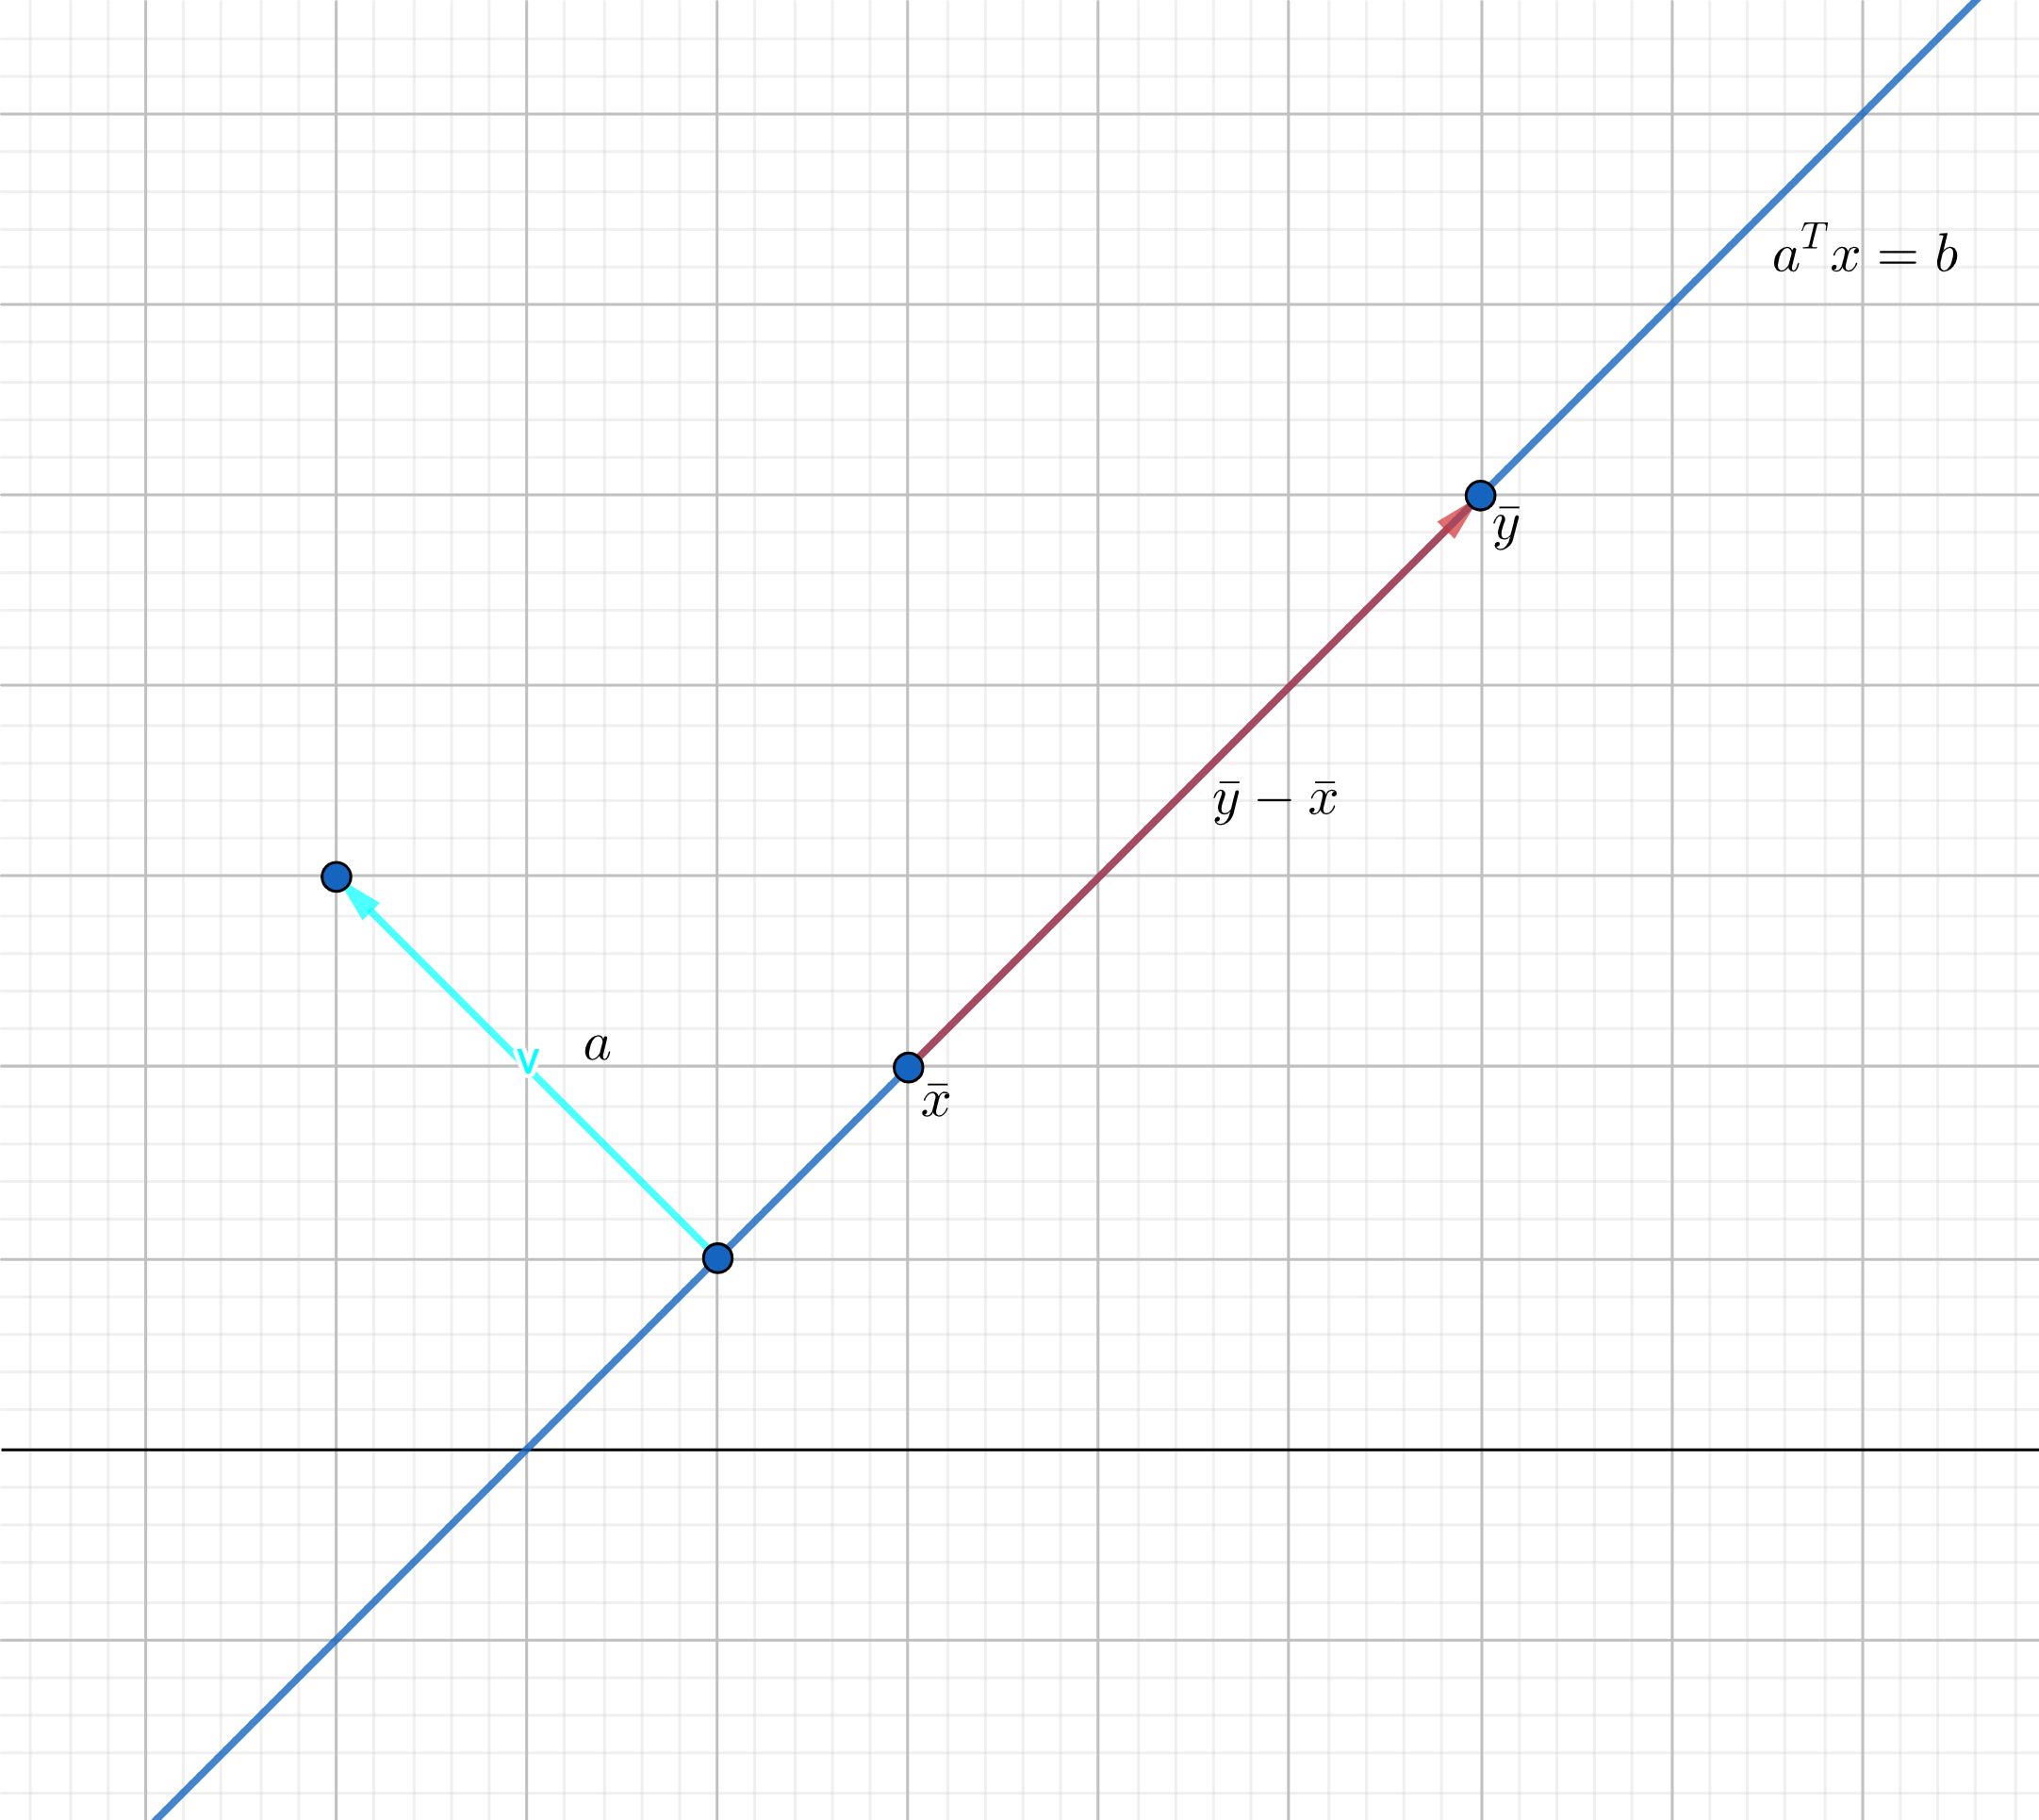
\includegraphics[scale=0.5]{angolirette.png}
\end{figure}

\noindent Questo ovviamente è valido per qualsiasi coppia di punti $\bar{x}$ e $\bar{y}$, quindi per ogni vettore che loro due formano.



\subsection{Rette, Semirette e Segmenti:} 

\paragraph{Retta:} Sia $\bar{x} \in \mathbb{R}^n$ un vettore (o punto, vettore e punto sono lo stesso oggetto), e sia d $\in \mathbb{R}^n$ (d di distanza) un altro vettore. Consideriamo un insieme parametrico di punti, con parametro $\lambda$: x($\lambda$) = $\bar{x}$ + $\lambda$ d. Al variare del parametro $\lambda \in \mathbb{R}$, $\bar{x}$ si muove sul grafico, disegnando una retta. Allora si ha:
\begin{equation*}
    R(\bar{x}, d) = \{x \in \mathbb{R}^n: x = \bar{x} + \lambda d, \lambda \in \mathbb{R}\}
\end{equation*}
è \textit{la retta passante per $\bar{x}$ e avente direzione d}

\paragraph{Semiretta:} Sia $\bar{x} \in \mathbb{R}^n$ un vettore, e sia d $\in \mathbb{R}^n$ un altro vettore. Definiamo l'insieme parametrico $x(\lambda) = \bar{x} + \lambda d$, ma stavolta $\lambda \in \mathbb{R}_+$. Allora:
\begin{equation*}
    S(\bar{x}, d) = \{x \in \mathbb{R}^n: x = \bar{x} + \lambda d, \lambda \in \mathbb{R}_+\}
\end{equation*}
è \textit{la semiretta passante per $\bar{x}$ e avente direzione d}. Nota che la semiretta è solo per $\lambda \in \mathbb{R}_+$, non è che se prendi $\lambda \in \mathbb{R}_-$ questa è la semiretta negativa e l'altra è la semiretta positiva. Tu prendi sempre $\lambda > 0$ e poi d decide il verso della retta, e quindi quale delle due semirette della retta devi prendere. Quindi la definizione \textit{generale} di semiretta è con $\lambda \in \mathbb{R}_+$, non era solo un esempio di semiretta, devi proprio sempre prendere $\lambda \in \mathbb{R}_+$, e poi se vuoi l'altra semiretta basta prendere d all'opposto, cioè se aveva componenti positive le prendi negative e hai l'altra semiretta.

\paragraph{Segmento:} Siano $\bar{x},\bar{y} \in \mathbb{R}^n$. Allora:
\begin{equation*}
    [\bar{x}, \bar{y}] = \{x \in \mathbb{R}^n: x = \lambda\bar{x} + (1 - \lambda)\bar{y}, \lambda \in [0,1]\}
\end{equation*}
Il segmento è una porzione limitata di retta. Questa definizione potrebbe richiamare la definizione di intervallo ma no non sono la stessa cosa perché l'intervallo è in $\mathbb{R}$ mentre questo è in un generico $\mathbb{R}^n$. Vediamo che si parla di un segmento perché per $\lambda = 0$ si ottiene $\bar{y}$, mentre per $\lambda = 1$ si ottiene $\bar{x}$. Per ogni valore tra 0 e 1 intermedi otteniamo i valori compresi tra gli estremi. Concludiamo dicendo che \textbf{Retta, Semiretta e Segmenti sono Insiemi Convessi}, che adesso definiremo. 

\subsection{Insieme Convesso:} Un insieme C $\subseteq \mathbb{R}^n$ è convesso quando, $\forall x,y \in C$, risulta [x,y] $\subseteq C$. Cioè quando, comunque presi due punti all'interno dell'insieme, il \textit{segmento} che li congiunge è contenuto \textit{interamente} nell'insieme stesso. 

\paragraph{Teorema:} L'intersezione di un numero finito qualsiasi di insiemi convessi è un insieme convesso. Dimostriamolo per due insiemi convessi. 

\subparagraph{Dimostrazione:} Prendiamo due insiemi convessi $C_1$ e $C_2$, e C = $C_1 \cap C_2$. Prendiamo x e y $\in$ C, ciò significa che x e y sono anche elementi sia di $C_1 e C_2$. Col fatto che questi sono convessi, il segmento che congiunge x e y è interamente contenuto in $C_1$ e anche in $C_2$. Quindi è interamente contenuto nell'intersezione tra i due, cioè C. Poiché il segmento che congiunge x e y è interamente contenuto in C, significa che C è convesso.



\subsection{Iperpiani e Semispazi:} 

\paragraph{Iperpiano:} Sia a $\in$ $\mathbb{R}^n$ e b $\in$ $\mathbb{R}$. Allora l'insieme:
\begin{equation*}
    H = \{x \in \mathbb{R}^n: a^{T}x = b\}
\end{equation*}
è un \textit{Iperpiano} in $\mathbb{R}^n$


\paragraph{Semispazi:} Sia a $\in \mathbb{R}^n$ e b $\in$ $\mathbb{R}$. Allora gli insiemi
\begin{equation*}
    S_{\geq} = \{x \in R^n: a^Tx \geq b\}
\end{equation*}
\begin{equation*}
    S_{\leq} = \{x \in R^n: a^Tx \leq b\}
\end{equation*}
Sono \textit{Semispazi}. Quindi un Iperpiano divide uno spazio in due Semispazi. Poniamoci questa domanda: un semispazio è un insieme convesso? Esempio:
$S_{\geq} = \{x \in R^n: a^Tx \geq b\}$ è convesso?

\subparagraph{Dimostrazione:} prendiamo
\begin{itemize}
    \item[I] $x \hspace{0.2cm} \text{t.c.} \hspace{0.2cm} a^Tx \geq b$ 
    \item[II] $y \hspace{0.2cm} \text{t.c.} \hspace{0.2cm} a^Ty \geq b$ 
\end{itemize}
Vogliamo far vedere che $\forall \lambda \in [0,1] \hspace{0.2cm} x(\lambda) = \lambda x + (1 - \lambda)y \in S_{\geq}$, giusto? Iniziamo moltiplicando (I) per $\lambda$ e (II) per $(1-\lambda)$, otteniamo:
\begin{itemize}
    \item[I] $\lambda a^Tx \geq \lambda b$ 
    \item[II] $(1-\lambda)a^Ty \geq (1-\lambda) b$ 
\end{itemize}
Adesso sommiamo termine a termine le due disuguaglianze:
\begin{equation*}
    \lambda a^Tx + (1-\lambda)a^Ty = a^Tx(\lambda) \geq \lambda b + (1-\lambda) b = b
\end{equation*} 
Da cui:
\begin{equation*}
    a^Tx(\lambda) \geq b
\end{equation*}
Quindi, poiché ci sono due punti x e y generici, all'interno del semispazio, e il loro segmento è interamente nello stesso semispazio, 
quindi il semispazio è un insieme convesso $S_{\geq}$ è un insieme convesso, e in generale \textit{tutti i semispazi sono insiemi convessi}.

\vspace{1cm}

\noindent Non solo, anche gli \textit{Iperpiano sono convessi}, dimostriamolo facilmente:
\begin{equation*}
    H = \{x \in R^n: a^Tx = b\}
\end{equation*}
Si tratta dell'intersezione dei due semispazi $S_{\leq} e S_{\geq}$, quindi essendo questi insiemi convessi, l'intersezione è convessa. Cioè tutti gli iperpiani sono convessi. Ovviamente questo risultato vale per $\mathbb{R}^n$ generico, quindi anche per $\mathbb{R}^2$ e $\mathbb{R}^3$: \textit{anche le rette e i piani sono insiemi convessi}. Bene, perché fare tutto questo? Perché questo adesso ci porta a dimsotrare che:

\paragraph{Teorema:} L'insieme ammissibile S di un problema di Programmazione Lineare (PL) è un insieme convesso. 

\subparagraph{Dimostrazione:} la regione ammissibile di un problema è data dall'intersezione di un numero finito di semispazi (vincoli con diseguaglianza) e iperpiani (vincoli con eguaglianze), quindi essendo sia i semispazi sia gli iperpiani convessi, la loro intersezione, cioè la regione ammissibile, è un insieme convesso.

\subparagraph{Nota:} Anche i due sottoinsiemi impropri di $\mathbb{R}^n$, cioè se stesso e l'insieme vuoto $\varnothing$, sono insiemi convessi. Anche un insieme composto da un solo punto è convesso. \textbf{Qualsiasi altro insieme composto da un numero FINITO di punti non è convesso}. Questo perché un segmento ha infiniti punti, quindi non può essere contenuto in un insieme con punti finiti.


\paragraph{Unione di insiemi convessi:} In generale l'unione di insiemi convessi non è convesso.


\section{Un problema di miscelazione:} Un'industria conserviera produce succhi di frutta (SF) mescolando polpa di frutta (P) e dolcificante (D). Il prodotto finale deve soddisfare alcuni requisiti sul contenuto di Vitamina C (V), Sali Minerali (S) e Zucchero (Z), che vediamo in questa tabella:
\begin{table}[h!]
    \centering
    \begin{tabular}{|c|c|c|c|c|}
    \hline
    & costo [\euro$_{cent}$/hg] & V [mg/hg] & S [mg/hg] & Z [g/hg]\\
    \hline
    P & 40 & 140 & 20 & 25\\
    \hline
    D & 60 & - & 10 & 50\\
    \hline
    SF & - & $\geq$ 70mg & $\geq$ 30mg & $\geq$ 75mg\\
    \hline
    \end{tabular}
\end{table}

\noindent Il nostro obiettivo è \textit{determinare le quantità ottime di P e D da miscelare}, per \textit{minimizzare i costi}. Come al solito, vogliamo matematicizzare questa situazione decisionale, e quindi dobbiamo porci la prima domanda che ci poniamo ogni volta in queste situazioni: \textit{cosa non conosciamo e vogliamo determinare?} Quelle saranno le nostre incognite. Noi non conosciamo le quantità di P e D da miscelare per ottenere abbastanza V,S e Z e spendere il meno possibile, quindi:
\begin{itemize}
    \item $x_1 \equiv$ q.tà [hg] di P da miscelare.
    \item $x_2 \equiv$ q.tà [hg] di D da miscelare.
\end{itemize}
In generale non c'è una regola per sapere quali sono le variabili, ma ci sono alcuni principi che ci aiutano:
\begin{itemize}
    \item Essere precisi nelle dimensioni delle quantità che usate.
    \item Vedere se riusciamo a esprimere attraverso le variabili ciò che serve esprimere, prima tra tutte la funzione obiettivo. In questo caso ci riusciamo. 
\end{itemize}
Bene, allora esprimiamola sta funzione obiettivo:
\begin{equation*}
    f(x) = Costo tot. = 40x_1 + 60x_2 
\end{equation*}
Bene, questa ricordiamoci che va minimizzata. Ora passiamo ai vincoli:
\begin{equation*}
    Vitamine tot. = 140 \frac{mg}{hg} \cdot x_1 hg  + 0\frac{mg}{hg} \cdot x_2 = 140x_1 mg \geq 70 mg
\end{equation*}
\begin{equation*}
    Sali tot. = 20x_1 + 10x_2 \geq 30
\end{equation*}
\begin{equation*}
    Zucchero tot. = 25x_1 + 50x_2 \geq 75
\end{equation*}
Manca una sempreverde condizione, che \textit{dobbiamo sempre ricordarci quando abbiamo a che fare con delle quantità}: \underline{esse non possono essere negative}.
\begin{equation*}
    x_1 \geq 0 
\end{equation*}
\begin{equation*}
    x_2 \geq 0 
\end{equation*}
Notiamo che $x_1 \geq 0$ è ridondante, poiché dalla prima condizione vediamo che $x_1 \geq \frac{1}{2}$. Disegnamo la zona ammissibile, nello stesso modo in cui abbiamo fatto la prima volta, e ci esce fuori:
\vspace{1cm}

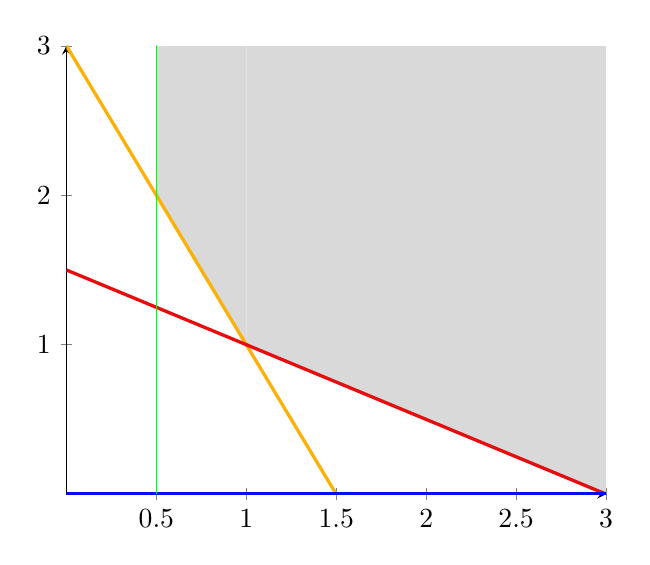
\begin{tikzpicture}
  \begin{axis}[
    axis lines=middle,
    xmin=0, xmax=3,ymin=0,ymax=3
  ]
  \addplot[thin,white, samples=300, domain=0:3, name path=A] {3}; %linea invisibile per far colorare pgfplots
  \addplot[very thick,yellow!70!red, samples=300, domain=0:3, name path=B] {(30 - 20*x)/10}; %passa per (0,3) e (3/2,0)
  \addplot[very thick,red!90!teal, samples=300, domain=0:3, name path=C] {(75-25*x)/50}; %passa per (0,3/5) e (3, 0)
  \addplot[very thick,blue!90!teal, samples=300, domain=0:3, name path=D] {0}; 
  \addplot[gray!30] fill between[of=A and B, soft clip={domain=1/2:1}];
  \addplot[gray!30] fill between[of=A and C,soft clip={domain=1:3}];
  \end{axis}
  \draw[green] (1.146,0) -- (1.145,5.7); % per disegnare la retta x = 1/2
\end{tikzpicture}

\noindent Notare che questa volta, a differenza della prima, la zona ammissibile è illimitata. Bene, ora passiamo alla funzione obiettivo. La funzione obiettivo $40x_1 + 60x_2 = k$ descrive un \textit{fascio di rette parallele}. Prendendo la retta di questo fascio $40x_1+60x_2 = 0$, vediamo che nessun punto di questa retta passa per la zona ammissibile. Questo perché mi sto domandando se esistono produzioni ammissibili, cioè coppie ($x_1,x_2$) che mi permettano di avere Costo tot. = 0 e rispettare i vincoli di V, S e Z totale, e ovviamente questo non è possibile. Proviamone un'altra, per esempio la retta del fascio che passa per il punto (3,0) intersezione della retta con l'asse x. Sostituendo $x_1 = 3$ e $x_2 = 0$ nell'equazione $40x_1 + 60x_1$ = k troviamo k = 120, cioè questa è la retta dei punti che mi fanno guadagnare 120. Ma vedo che posso trovare anche di meglio, spostandola più in basso (ricordiamo che stiamo cercando di minimizzare la funzione). Provando le altre intersezioni rimaste (in zona ammissibile) vediamo che il miglior punto è (1,1), dove k = 100, e spendiamo il minimo possibile. Se io volessi spendere meno di 100 devo considerare rette sotto la retta del fascio per cui ottengo 100, ma nessuna di queste passa per la zona ammissibile.

\subparagraph{Nota (penso che dopo il professore ce lo dirà formalmente):} \textit{i punti di ottimizzazione} (sia di massimizzazione che di minimizzazione) si trovano SEMPRE in un punto di intersezione tra due rette che formano la zona ammissibile, quindi cerca in quei punti se vuoi trovare il valore ottimo!


\subparagraph{Domanda di un alunno:} Professore ma se il fascio di rette generato dalla funzione obiettivo è parallelo a un vincolo, avremmo un insieme di punti come soluzione? Ha risposto di sì, ma tanto a te sempre l'intersezione ti interesserebbe, anche in quel caso, perché anche in quel caso puoi trovare un punto intersezione tra le rette.







\subsection{Altro esempio:}
\begin{equation*}
    S = \{(x,y) \in R^2, x^2 + y^2 \geq 1, x + y \geq 2\}
\end{equation*}
Vediamo che S, essendo l'intersezione tra l'area al di fuori del cerchio e un sottoinsieme di quest'area (cioè  $x + y \geq 2$), è proprio uguale a quest'ultima. Essendo quest'ultima convessa, anche S è convesso. Notare che il fatto che un'area sia contenuta in un'altra, porta l'equazione di quest'ultima ad essere ridondante, come in questo caso è l'equazione del cerchio. Bene, ora classifichiamo S:
\begin{itemize}
    \item S è un problema di ottimizzazione? Sì, perché può essere scritto nella forma:
    \begin{equation*}
        min f(x)
    \end{equation*}
    \begin{equation*}
        x \in S = \{(x,y) \in R^2, x^2 + y^2 \geq 1, x + y \geq 2\}
    \end{equation*}
    \item S è un problema di Programmazione Matematica? Sì, perché esso è definito solo da disuguaglianze
    \item S è un problema di PL? No, perché c'è un'equazione non lineare. 
\end{itemize}
Quindi questo è un problema di PNL. Notare che \textit{non importa che l'equazione che rende il problema non lineare sia ridondante, non possiamo pensare di non considerarla} solo perché è ridondante! Comunque non è lineare, anche se se la eq. ridondante venisse eliminata il problema diventerebbe PL, perché in questo caso staremo definendo un'altra S e quindi un altro problema.


\newpage

\section{Esercizi:} 

\paragraph{1:} Una industria è specializzata nella fabbricazione di un prodotto per il fai-da-te in due qualità differenti standard e deluxe. Ciascuna unità di prodotto richiede (tra le altre) una fase di smerigliatura ed una di pulitura. In tabella sono riportati i tempi di lavorazione delle due fasi in ore (per unità di prodotto); i prezzi di vendita in e (per unità di prodotto)
\begin{table}[h!]
    \centering
    \begin{tabular}{|c|c|c|}
    & standard &  deluxe \\
    smerigliatura [h/u] & 4 & 3\\
    pulitura [h/u] & 2 & 5\\
    prezzo [\euro/u] & 10 & 15
    \end{tabular}
\end{table}
Le macchine adibite ai due processi di smerigliatura e pulitura lavora per, risp., 80 e 60 ore per settimana. Scrivere un problema di PL che consenta di determinare il piano ottimo di produzione settimanale (ipotizzando che tutto ciò che viene prodotto sia venduto).
\begin{itemize}
    \item Individuare le variabili di decisione specicandone precisamente l'unità di misura
    \item Scrivere la funzione che si vuole massimizzare o minimizzare specicandone precisamente l'unità di misura
    \item Scrive i vincoli che limitano le scelte possibili specicandone precisamente l'unità di misura
\end{itemize}


\subparagraph{Risposta:} 

\


\begin{figure}[h!]
    \centering
    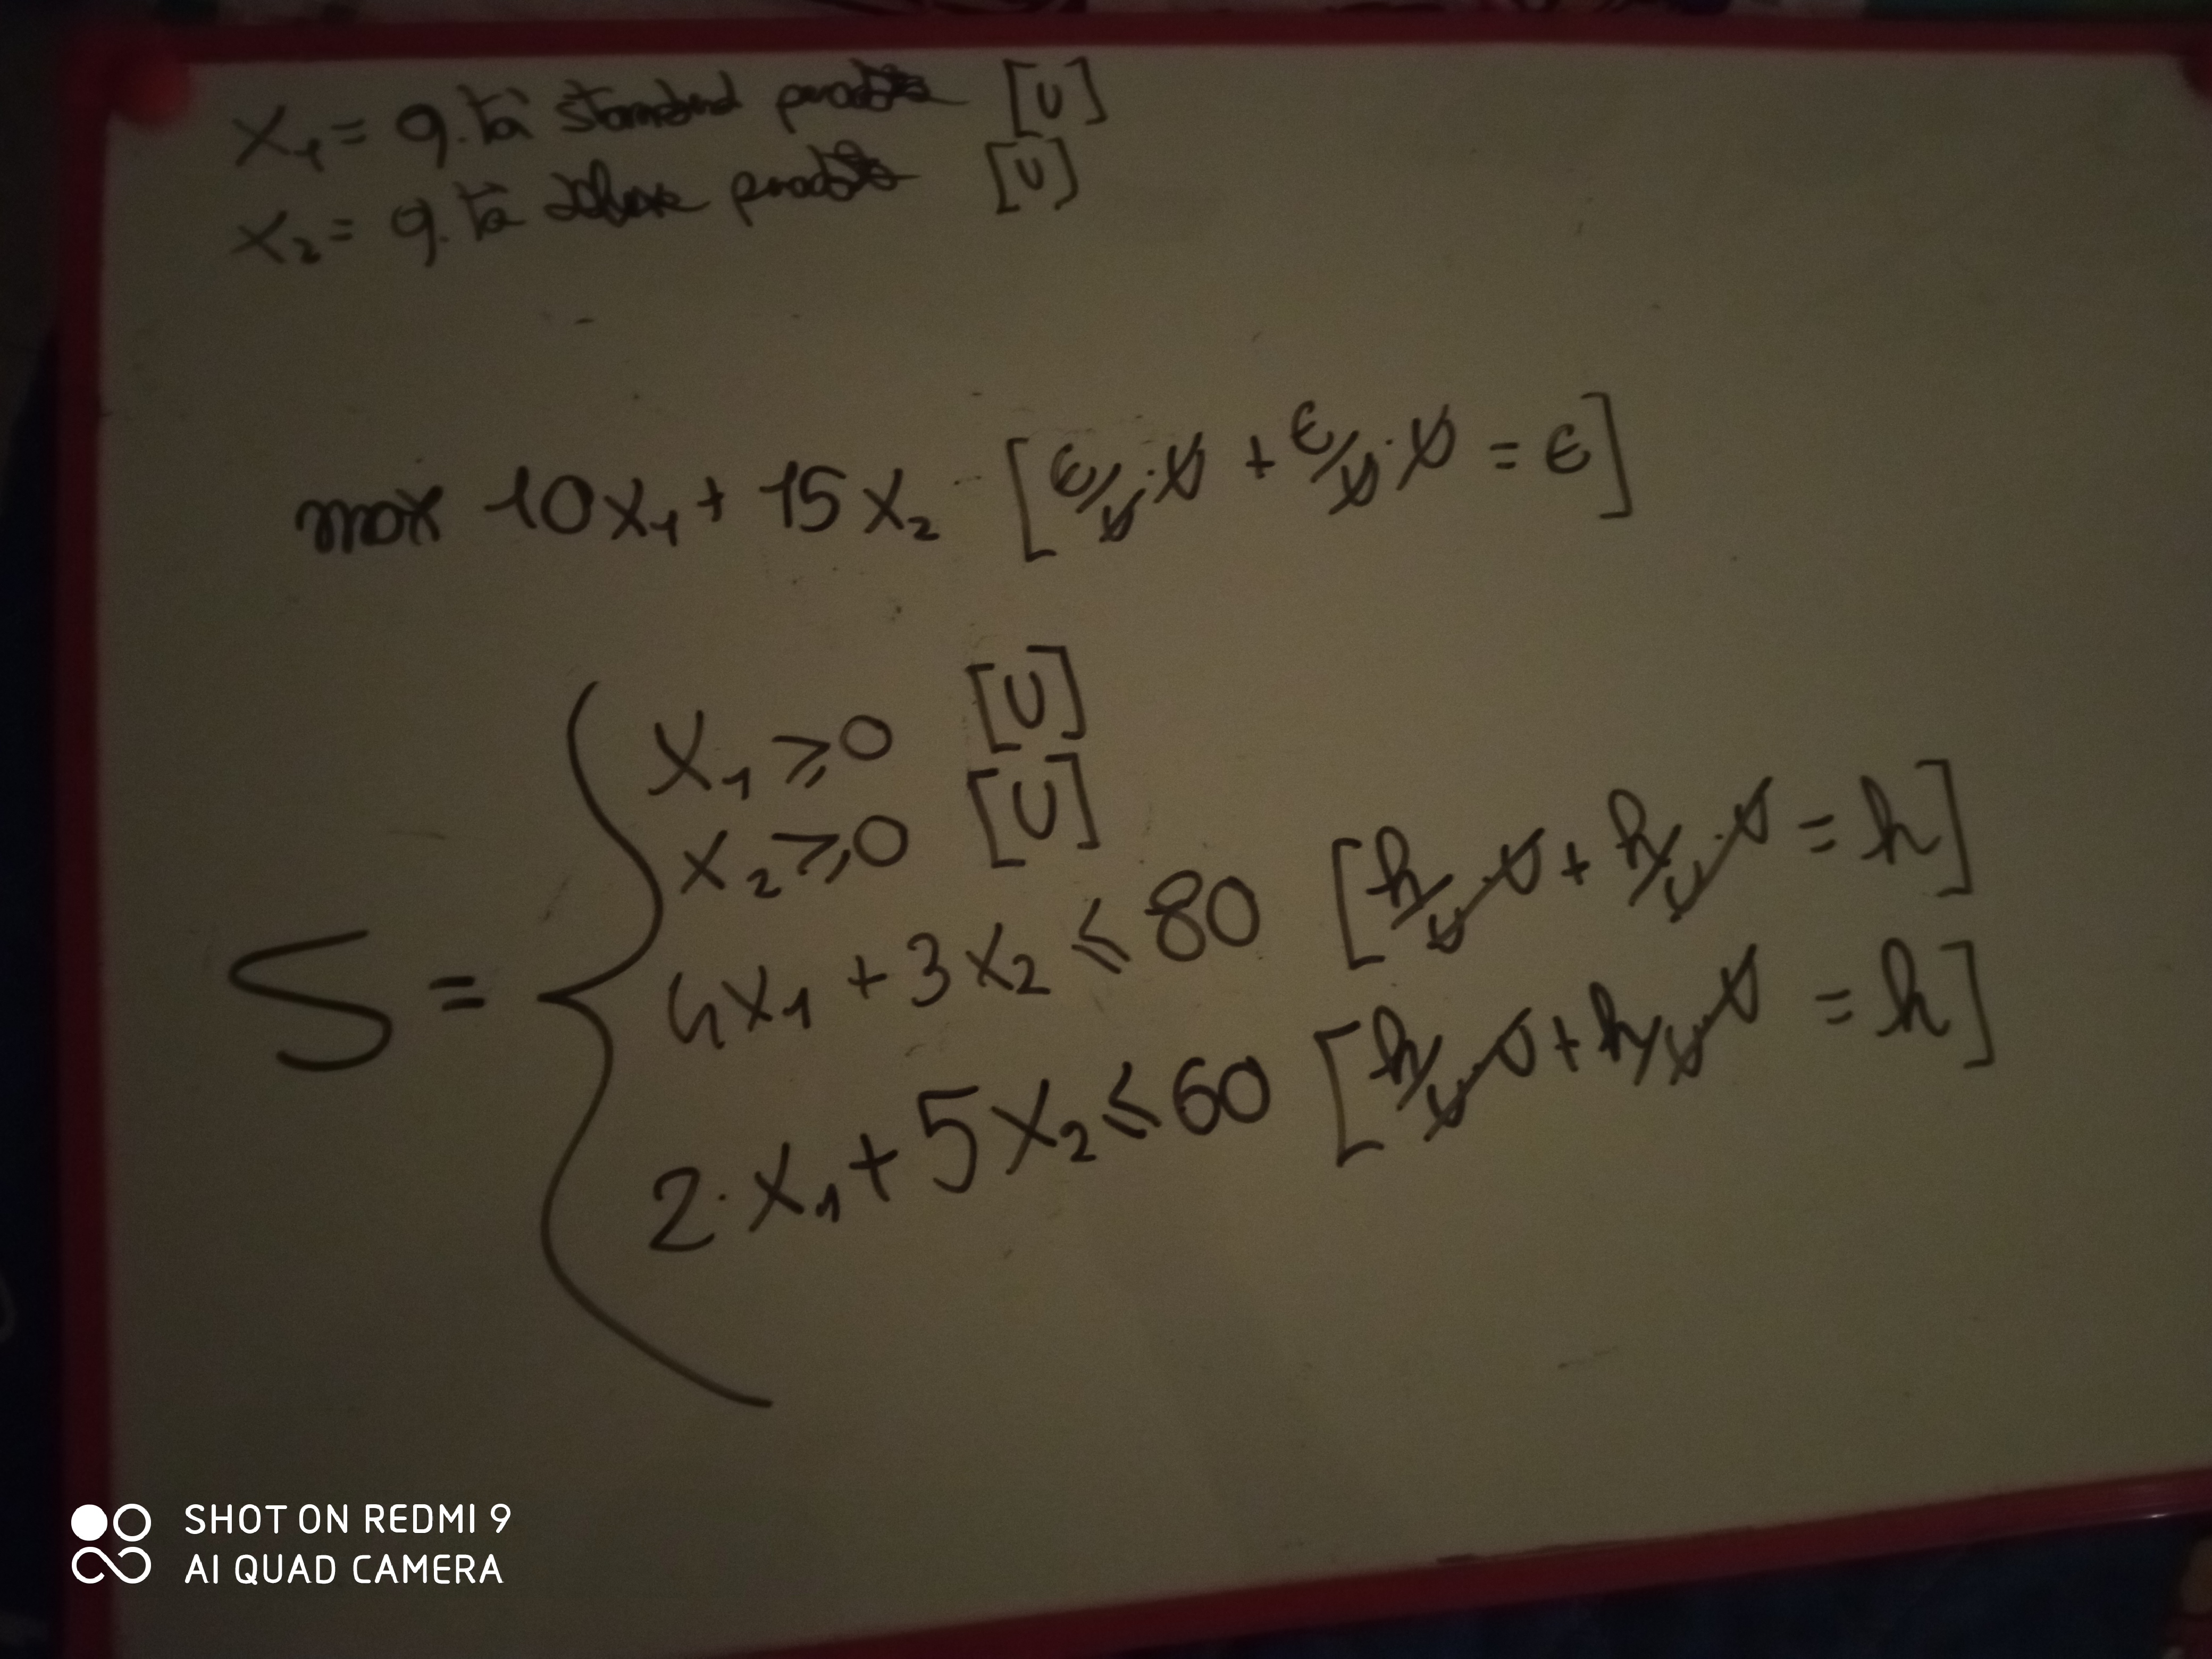
\includegraphics[scale=0.05]{esercizio2.jpg}
\end{figure}
ATTENZIONE!!! Le variabili di decisione $x_1$ e $x_2$ non sono unità MA unità per settimana. In conseguenza di ciò, i vincoli sono in ore per sett. e la f.ob. in euro per sett. \textcolor{red}{CORREGGERE!!!!!!!!!}

\paragraph{2.} Dato il seguente sistema di disuguaglianze lineari (che rappresenta la regione ammissibile di un ipotetico problema di PL)
\begin{equation*}
    \begin{cases}
        \text{$x1 + 3x2 + 2x3 \leq 3$}\\
        \text{$4x1 + x2 + x3 \geq 5$}\\
        \text{$x3 \leq 1$}\\
        \text{$x1 \geq 0$}\\
        \text{$x3 \geq 0$}
    \end{cases}
\end{equation*}
\begin{itemize}
    \item Quanti vincoli sono attivi in (0, 1, 0)?
    \item Quanti vincoli sono violati in (0, 1, 0)? Il punto (0, 1, 0) è ammissibile?
    \item Quanti vincoli sono attivi in (1, 0, 1)? Il punto (1, 0, 1) è ammissibile?
    \item Quanti vincoli sono attivi in (1, 0, 1)?
    \item Il punto (1, 0, 1) è ammissibile?
\end{itemize}

\subparagraph{Risposta:} 

\

\begin{figure}[h!]
    \centering
    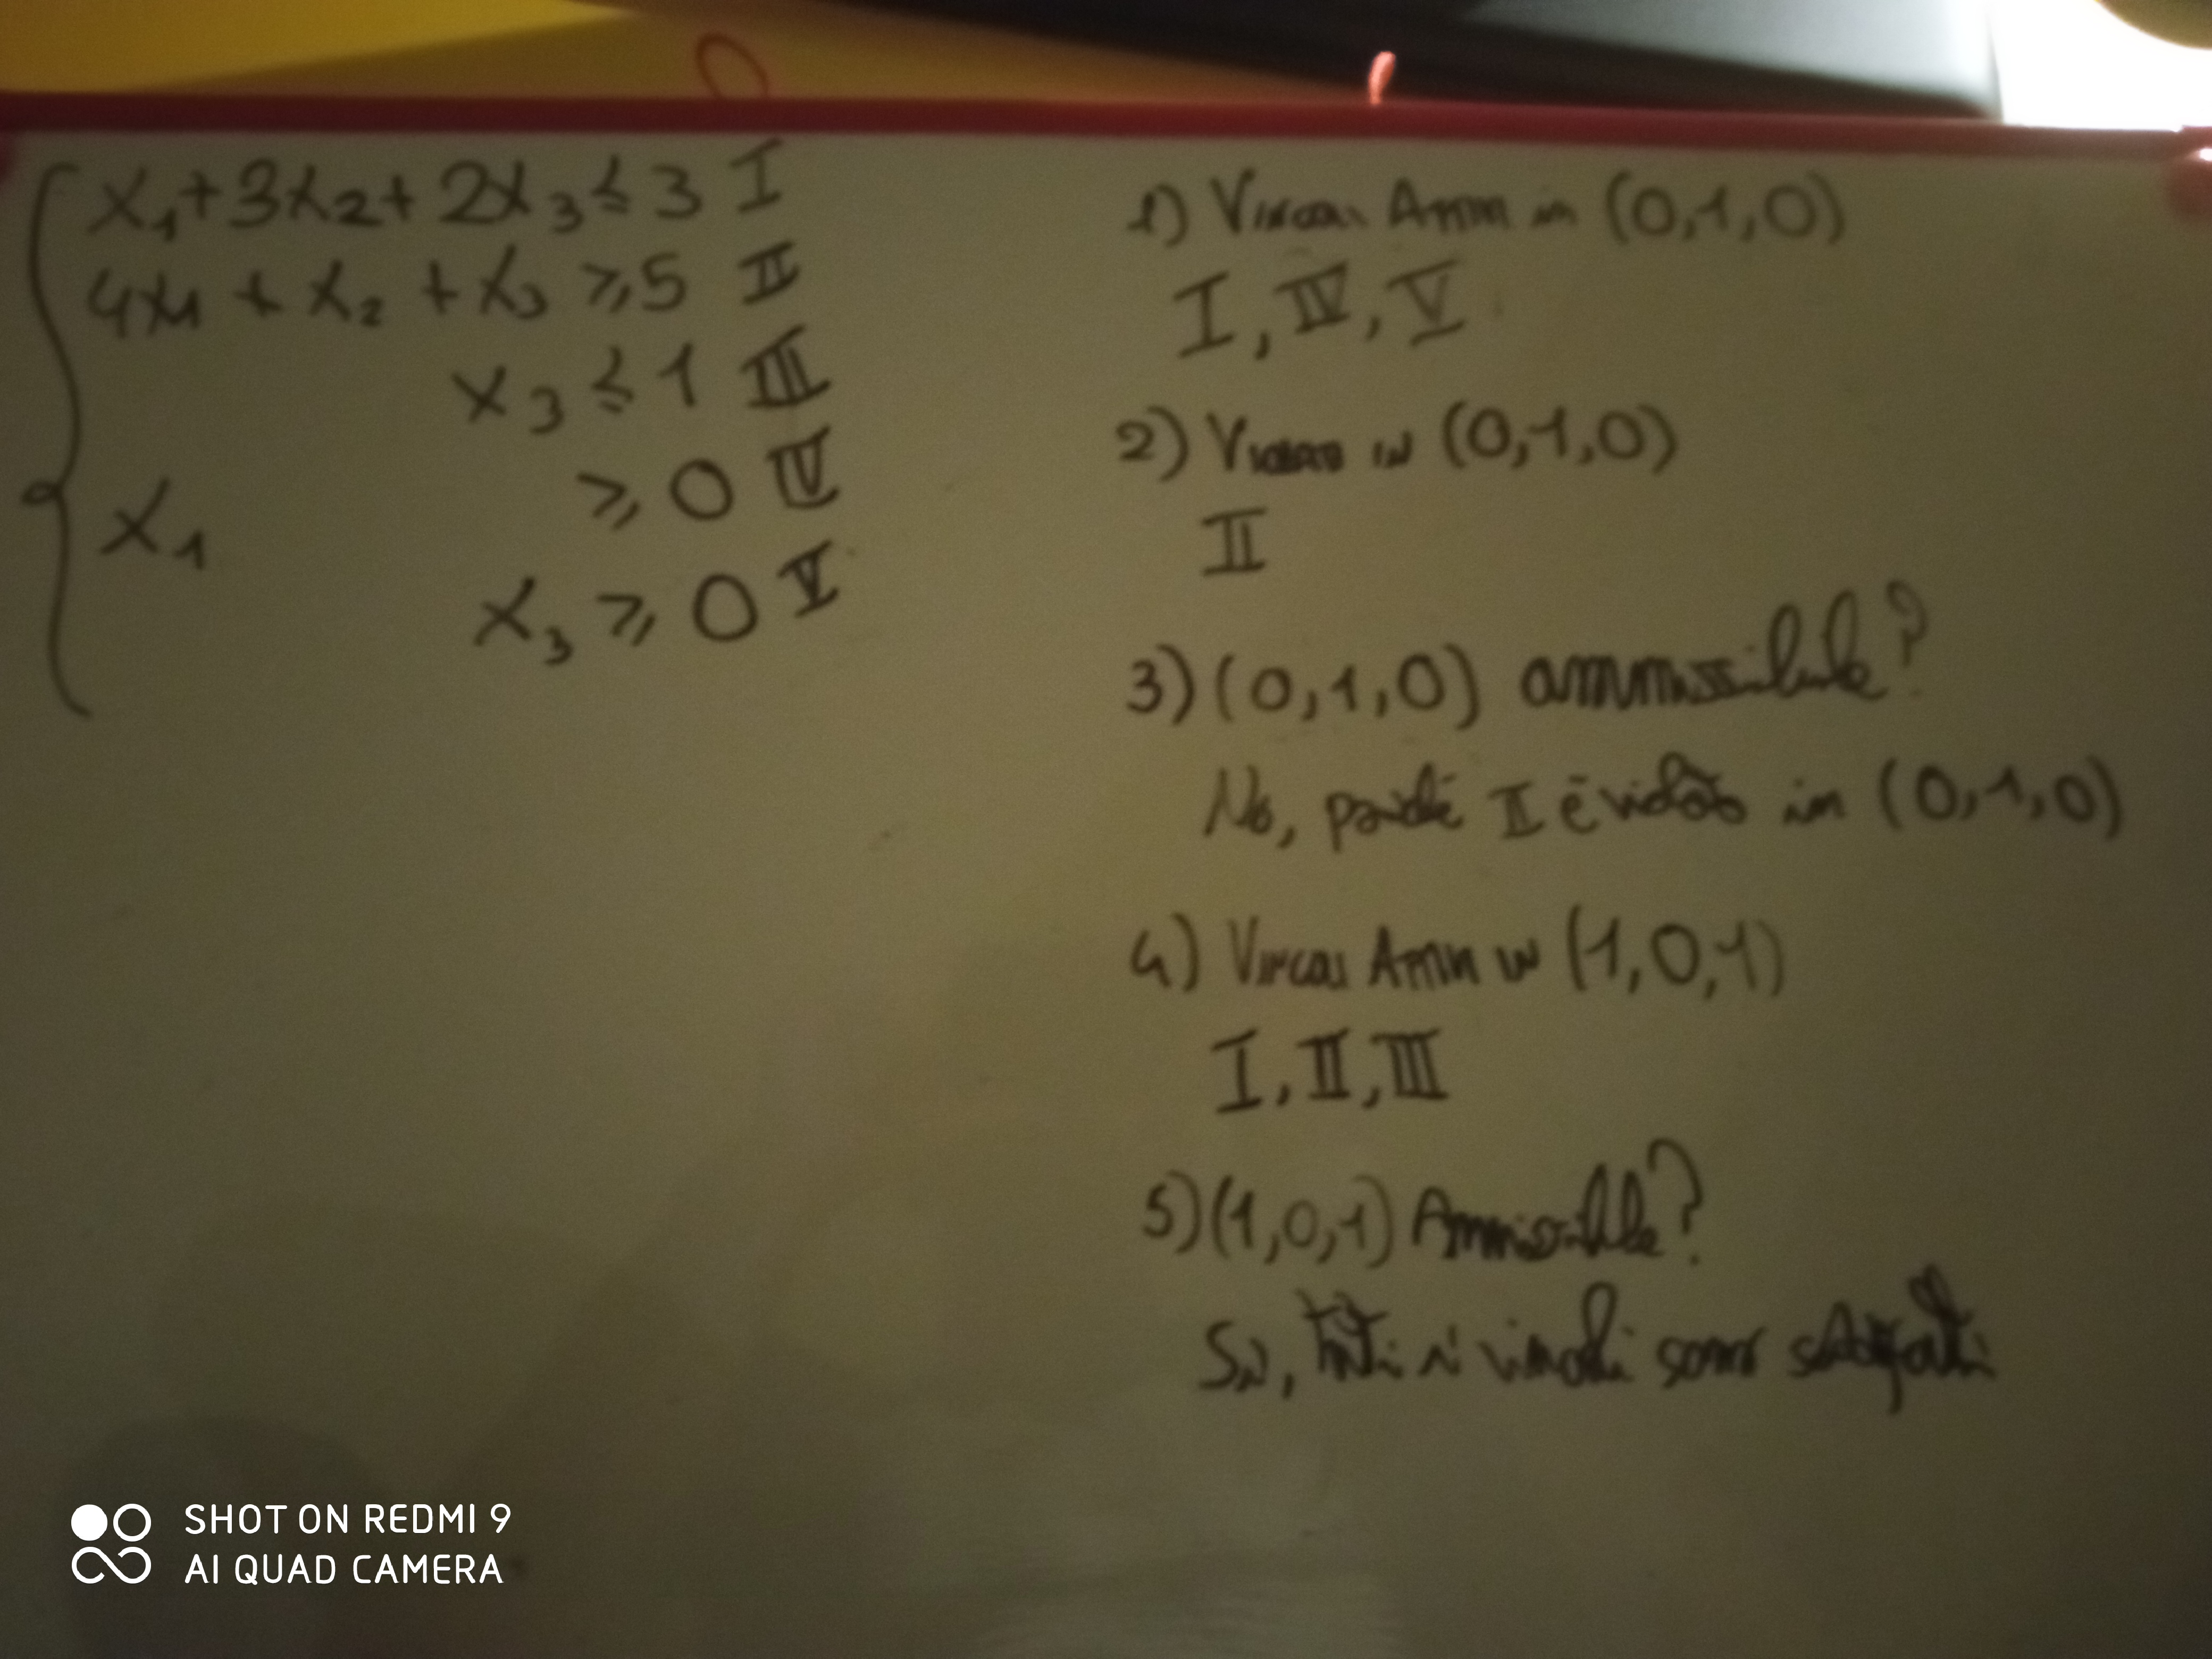
\includegraphics[scale=0.05]{esercizio1.jpg}
\end{figure}



























\section{Poliedri e Politopi:} L'intersezione di un numero finito di semispazi chiusi e iperpiani è detto \textbf{poliedro}. Se un poliedro si può racchiudere in una sfera di centro l'origine e raggio abbastanza grande è limitato e si dice che è un \textbf{politopo}. Facciamo degli esempi:
\begin{itemize}
    \item In $\mathbb{R}^2$ il primo quadrante è un poliedro illimitato
    \item L'insieme vuoto è un poliedro, anzi essendo limitato è un politopo.
    \item Tutto $\mathbb{R}^n$ è un poliedro. 
\end{itemize}

\paragraph{Teorema (caratterizzazione dei poliedri):} un insieme P $\subseteq \mathbb{R}^n$ è un poliedro sse $\exists A \in \mathbb{R}^{m\times n}, b \in \mathbb{R}^m$ t.c.:
\begin{equation*}
    P = \{x \in \mathbb{R}^n: Ax \geq b\}
\end{equation*}
Che, se ricordiamo, è proprio nella forma dell'insieme delle soluzioni ammissibili di un problema di PL in forma generale. Ciò significa che \textbf{l'insieme ammissibile di un problema di PL è un poliedro}. Inoltre da questo possiamo dimostrare che:
\begin{itemize}
    \item $\mathbb{R}^n$ è un poliedro, poiché può essere scritto come:
    \begin{equation*}
        P = \{x \in \mathbb{R}^n: 0^Tx \geq 0\}
    \end{equation*}
    Vediamo che per qualunque x in $\mathbb{R}^n$ il vincolo è soddisfatto, quindi si tratta proprio di tutto $\mathbb{R}^n$
    \item $\varnothing$ è un poliedro, poiché può essere scritto come l'intersezione di due o più qualsiasi disequazioni incompatibili (esempio $3x \geq 0$ e $3x \leq -12$). Che quindi in forma matriciale si scrivono nella forma richiesta per i poliedri.
\end{itemize}


\subsection{Vertici:}

\paragraph{Definizione di Vertice:} dato un insieme convesso - non per forza poliedrale - C, diciamo che x $\in$ C è vertice di C quando NON è possibile determinare due punti y,z $\in$ C t.c. y $\neq$ z, y $\neq$ x, x $\neq$ z, per cui:
\begin{equation*}
    x = \lambda y + (1 - \lambda)z \hspace{0.5cm} \text{Per qualche $\lambda \in (0,1)$}
\end{equation*}
Quindi, ricordandoci la definizione di segmento, la definizione a parole dice questo: prendo un punto di C, se è un vertice allora non deve essere possibile determinare un segmento di estremi y e z (anche loro in C e distinti sia da x che tra di loro) che sia tutto contenuto in C e per cui passi x.


\newpage 

Graficamente: 
\begin{figure}[h!]
    \centering
    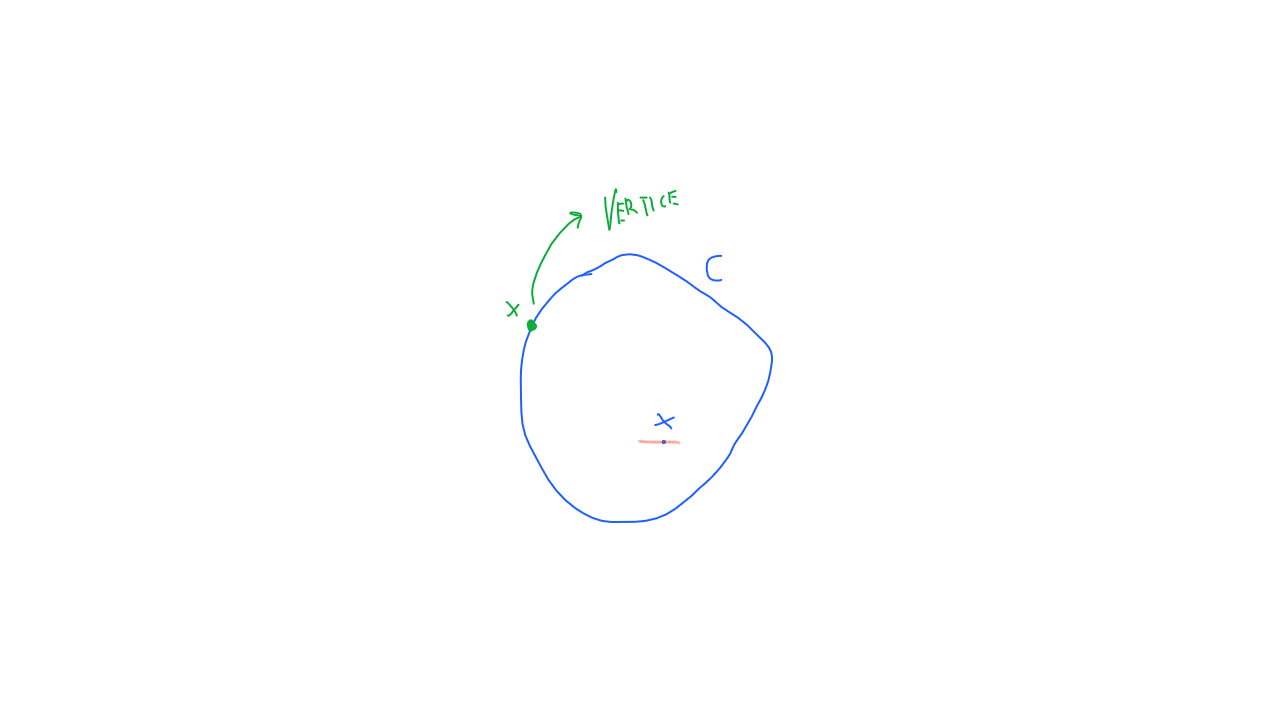
\includegraphics[scale=0.5]{vertice.png}
    \caption{Vediamo come il punto x in blu, all'interno dell'insieme, non sia un vertice, poiché posso determinare altri due punti all'interno di C, che sono estremi di un segmento in cui x è contenuto. Mentre la x in verde è un vertice, perché non riesco a trovare un segmento, con estremi altri due punti di C, che contiene x al suo interno} 
\end{figure}

\noindent Vediamo ora degli esempi di vertici nel caso poliedrale. Innanzitutto diciamo che per i poliedri i vertici sono quelli che intuitivamente uno si immagina. Facciamo un esempio con questo P:
\begin{figure}[h!]
    \centering
    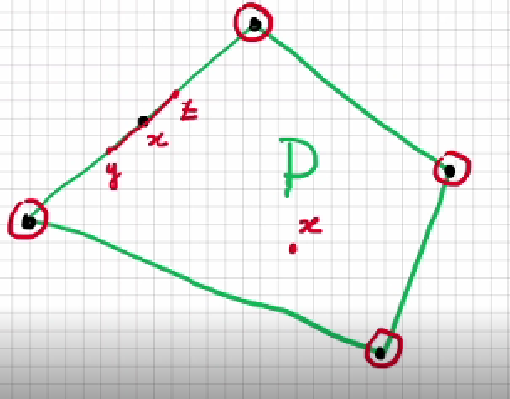
\includegraphics[scale=0.5]{PoliedroVertici.png}
\end{figure}

\noindent Vediamo che anche per i punti sui lati riesco a trovare un segmento, ma non lo trovo per quei 4 punti, quindi solo questi ultimi sono vertici. Questi 4 punti hanno una particolarità: sono all'intersezione tra un certo numero di rette (in $\mathbb{R}^2$), piani ($\mathbb{R}^3$) o iperpiani ($\mathbb{R}^n$). Quindi, stando a questo disegno, sembrerebbe che se l'insieme è un poliedro i vertici sono finiti, mentre nel convesso generale (ad esempio un cerchio) essi sono infiniti. In effetti, posso aumentare quanto voglio i lati del poliedro, ma affinché resti un poliedro il numero di semispazi e iperpiani che lo definiscono devono essere FINITI, quindi le facce non possono essere infinite. Dimostreremo più avanti che i vertici di un poliedro sono in numero finito.

\subparagraph{Nota:} numero finito di vertici non significa non nullo. Esistono poliedri con 0 vertici, il poliedro vuoto ne è un esempio, ma non l'unico. Un altro esempio è:
\begin{equation*}
    P = \{x \in R^2: x_1 \geq 0\}
\end{equation*}
Che essenzialmente è l'insieme dei punti nel I e nel IV quadrante nel piano, e vediamo che non ha vertici.

\paragraph{Caratterizzazione dei vertici di P (Teorema di Equivalenza)} 
Il discorso è che, seppur la definizione vale anche per i poliedri (essendo essi convessi), è molto geometrica e al negativo (il vertice NON deve avere una proprietà), perciò non è utile computazionalmente per trovare i vertici. Vediamo come caratterizzare la ricerca dei vertici nel caso dei poliedri: consideriamo un poliedro
\begin{equation*}
    P = \{x \in \mathbb{R}^n: Ax \geq b\}
\end{equation*}
Sappiamo che la matrice A ha m righe e n colonne, mentre b è un vettore di m colonne. Indichiamo con $a_i^T$, i = 1,...,m, le righe\footnote{Nei corsi MAT09 i vettori sono solo colonne. Siccome qua stiamo prendendo una riga, prendiamo la trasposizione. Quindi si tratta solo di una notazione per indicare le righe.} della Matrice A. Perciò:
\begin{equation*}
    Ax \geq b \Longleftrightarrow a_i^Tx \geq b_i \forall i \in \{1,...,m\}
\end{equation*}
Altra cosa da definire che ci serve: l'insieme degli indici dei vincoli attivi. Noi prendendo un qualsiasi punto $\bar{x} \in \mathbb{R}^n$, e un poliedro P = \{$x \in \mathbb{R}^n: Ax \geq b$\} con matrice A $\in \mathbb{R}^{m\times n}$, abbiamo, per ogni riga della matrice, 3 possibilità:
\begin{itemize}
    \item $a_i^T\bar{x} \geq b_i$
    \item $a_i^T\bar{x} \leq b_i$
    \item $a_i^T\bar{x} = b_i$
\end{itemize}
Allora, dato questo punto, non per forza appartenente al poliedro, $\bar{x} \in \mathbb{R}^n$, e il poliedro stesso P = \{$x \in \mathbb{R}^n: Ax \geq b$\} definiamo \textit{Insieme degli indici dei vincoli attivi} il seguente insieme:
\begin{equation*}
    I(\bar{x}) = \{i: a_i^T\bar{x} = b_i\}
\end{equation*}
Quindi l'insieme degli indici per i quali $\bar{x}$ soddisfa all'uguaglianza il vincolo. 

\subparagraph{Nota:} Il prof si riferirà al vincolo o alla riga della matrice corrispondente a quel vincolo nella stessa maniera. Quindi il vincolo è linearmente indipendente quando le righe della matrice sono linearmente indipendenti

\vspace{1cm}

\noindent Bene, siamo pronti per la caratterizzazione dei vertici nel caso di un poliedro. Dato un poliedro P = \{$x \in \mathbb{R}^n: Ax \geq b$\} e un punto $\bar{x} \in P$, $\bar{x}$ è un vertice di P sse esistono n righe $a_i^T$ della matrice A con $i \in I(\bar{x})$, quindi una sottomatrice di A composta dalle righe che hanno indici i appartententi a $I(\bar{x})$, che sono lin. indipendenti. Ovvero sse
\begin{equation*}
    rg(a_i^T)_{i \in I(\bar{x})} = n
\end{equation*}
Quindi il rango della sottomatrice di A composta dalle righe che hanno indici $i \in I(\bar{x})$ deve essere pari a n. Grazie a questa caratterizzazione algebrica riusciamo a calcolare tutti i vertici di un poliedro. Il numero n sta per la dimensione dello spazio, cioè n è il numero di colonne della matrice o equivalentemente il numero di variabili è n. Quindi attenzione che in questo caso $a_i^T$ è una matrice.


\subparagraph{Dimostrazione (per assurdo):} dimostriamo in due passi. Primo passo: supponiamo che la tesi non sia vera. Quindi:
\begin{equation*}
    \bar{x} \hspace{0.2cm} \text{è un vertice} \implies rg(a_i^T)_{i\in I(\bar{x})} < n
\end{equation*}
Se il rango è minore di n, allora:
\begin{equation*}
    a_i^Tx  = 0 \hspace{1cm} \text{con i $\in I(\bar{x})$}
\end{equation*}
ha infinite soluzioni oltre quella banale (ricorda che $a_i^T$ è la matrice di tutte le righe con indice in $I(\bar{x})$). Ad esempio $\exists$ d $\in \mathbb{R}^n$, $d \neq 0$ che è soluzione. Cioè:
\begin{equation*}
    a_i^Td = 0  \hspace{1cm} \text{con i $\in I(\bar{x})$}
\end{equation*}
Adesso abbiamo un punto $\bar{x}$ e un vettore d. Un punto e un vettore definiscono una retta. Adesso definisco due punti y = $\bar{x} + \epsilon d$, z = $\bar{x} - \epsilon d$, distinti da $\bar{x}$ e tra loro, con $\epsilon > 0$. Questi punti che ho definito passano sulla retta identificata da $\bar{x}$ e d. Precisamente sono gli estremi di un segmento di cui $\bar{x}$ è il punto mediano.
\begin{figure}[h!]
    \centering
    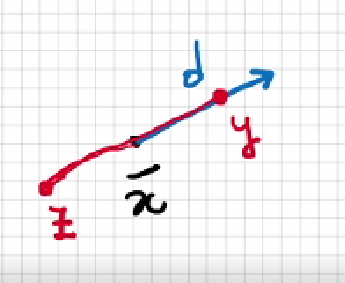
\includegraphics[scale=0.5]{dimostrazione.png}
\end{figure}
Quindi $\bar{x} = \frac{1}{2}y + \frac{1}{2}z$. Adesso vediamo s x e y stanno o pure no nel poliedro in cui sta $\bar{x}$. Consideriamo due casi:
\begin{itemize}

    \item $i \in I(\bar{x})$. Ma per questi indici sappiamo che $a_i^T\bar{x} = b_i$ e $a_i^Td = 0$, quindi, nel caso di y, utilizzando la sua espressione prima definita:
    \begin{equation*}
        a_i^Ty = a_i^T\bar{x} + \epsilon a_i^T d = b_i
    \end{equation*}
    Tutti i vincoli quindi che sono soddisfatti all'uguaglianza in $\bar{x}$ lo sono anche in y. Idem per z, infatti:
    \begin{equation*}
        a_i^Tz = a_i^T\bar{x} - \epsilon a_i^T d = b_i
    \end{equation*}
        Perciò y e z soddisfano all'uguaglianza i vincoli del poliedro che anche $\bar{x}$ soddisfa all'uguaglianza. E invece i vincoli che non soddisfa all'uguaglianza? Cioè quelli che soddisfa col $>$? Lo vediamo al prossimo punto. 
    
    \item i $\notin I(\bar{x})$. In questo caso sappiamo che $a_i^T\bar{x} > b_i$. Perché? Bhe se i $\notin I(\bar{x})$ vuol dire che $a_i^T\bar{x} \neq b_i$, inoltre, poiché $\bar{x} \in P$ e P = \{$x \in \mathbb{R}^n: Ax \geq b$\} non può valere $a_i^T\bar{x} < b_i$, quindi per forza di cose $a_i^T\bar{x} > b_i$. Definisco ora il semispazio $S_i = \{x \in R^n: a_i^Tx \geq b_i\}$, che non è nient'altro che il semispazio che ha come diseguaglianza una delle righe della matrice (quindi tutti gli $S_i$, cioè per ogni i, comporranno l'intero P). Vediamo che, per quanto detto sopra, $\bar{x}$ è un punto interno all'insieme $S_i$. Siccome è interno a $S_i$ posso definire un intorno aperto di $\bar{x}$ con raggio $>$ 0 che è tutto contenuto in $S_i$, cioè $\exists \epsilon_i > 0 : B(\bar{x}, \epsilon_i) \subseteq S_i$ cioè $\epsilon_i$ raggio e B palla di centro $\bar{x}$ e raggio $\epsilon_i$. E questo lo posso fare per tutte le i $\notin I(\bar{x})$, definendo il corrispettivo $S_i$ e trovando il raggio $\epsilon_i$. Il numero di i è ovviamente finito, quindi troverò un numero finito di raggi $\epsilon_i$. Di questi prendo il minimo $\rho = min(\epsilon_i) > 0$. Avendo trovato il raggio più piccolo, posso essere certo nell'affermare che:
    \begin{equation*}
        B(\bar{x}, \rho) \subset S_i \hspace{1cm} \forall i \notin I(\bar{x})
    \end{equation*}
    Cioè ho trovato una palla che è contenuta dentro tutti i vincoli di tutti gli $S_i$. Cioè di tutti i vincoli di P che non sono soddisfatti all'uguaglianza da $\bar{x}$ (per quelli c'è il punto precedente).
    \begin{figure}[h!]
        \centering
        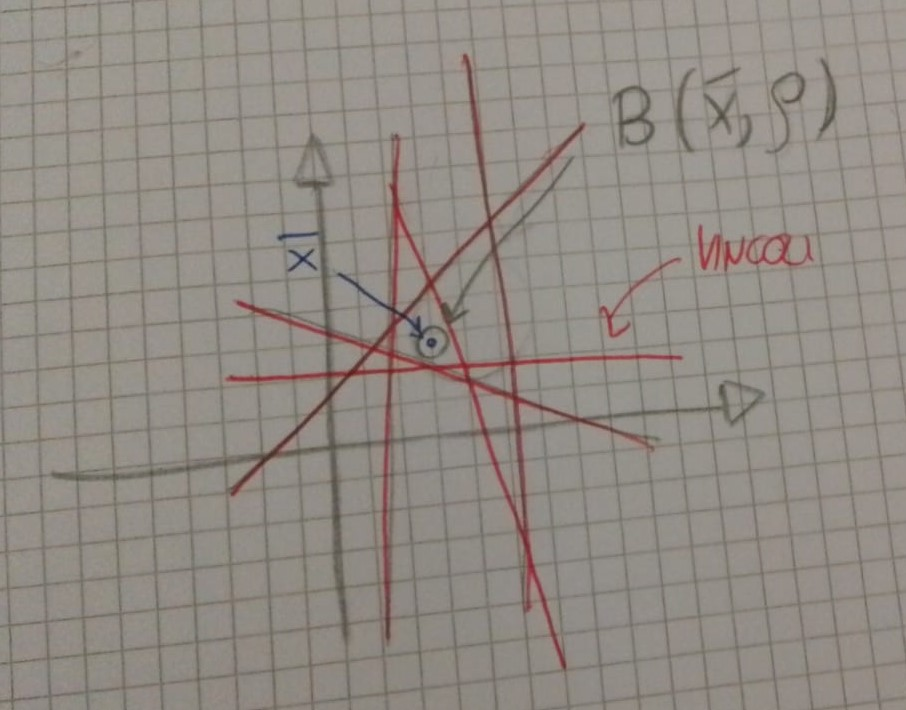
\includegraphics[scale=0.3]{pallarho.jpeg}
    \end{figure}
    Adesso se riprendiamo il segmento che aveva come estremi y = $\bar{x} + \epsilon d$ e z = $\bar{x} - \epsilon d$, e ci ricordiamo che questo aveva come punto medio $\bar{x}$, ci basterà prendere $\epsilon \leq \rho$ per avere un segmento che ha come punto medio $\bar{x}$ ed è tutto contenuto nella palla B($\bar{x}$, $\rho$). Attezione!! Quest'ultimo $\epsilon$ non è il raggio $\epsilon_i$ ma riguarda la lunghezza del segmento. Bene quindi abbiamo trovato e y e z soddisfano anche loro $a_i^Tx > b_i$. Cioè:
    \begin{equation*}
        a_i^Tz > b_i \hspace{1cm} a_i^Ty > b_i
    \end{equation*}
    Come x.
\end{itemize}
Perciò abbiamo trovato che quando $i \in I(\bar{x})$ per qualunque valore di $\epsilon$ i vincoli che erano soddisfatti all'uguaglianza da $\bar{x}$ saranno soddisfatti all'uguaglianza anche da y e z; mentre quando $i \notin I(\bar{x})$, per qualunque $\epsilon \leq \rho$, i vincoli che erano soddisfatti strettamente ($>$) da $\bar{x}$ saranno soddisfatti strettamente ($>$) da y e z. Quindi cosa ci ritroviamo:
\begin{equation*}
    \bar{x} \in P, \text{e per $\epsilon \leq \rho y,z \in P$}
\end{equation*}a
Ma questo è un ASSURDO! Perché abbiamo trovato un segmento tutto contenuto in P per cui passa $\bar{x}$, ma abbiamo supposto che $\bar{x}$ fosse un vertice. 

\vspace{1cm} Ora ci rimane da fare l'implicazione nell'altro senso. Anche qui supponiamo la tesi non sia vera e dimostriamo per assurdo:
\begin{equation*}
    rg(a_i^T)_{i\in I(\bar{x})} < n \implies \bar{x} \hspace{0.2cm} \text{non è un vertice}
\end{equation*}
Se $\bar{x}$ non è un vertice vuol dire che $\exists y,z \in P$ distinti da $\bar{x}$ e tra loro tali che:
\begin{equation*}
    \bar{x} = \lambda y + (1 - \lambda)z \hspace{1cm} \lambda \in (0,1)
\end{equation*}
Qui prendiamo il solo caso: $i \in I(\bar{x})$, quindi parliamo dei vincoli $a_i^T\bar{x} = b_i$. Noi sappiamo, poiché y e z appartengono a P, che sicuramente:
\begin{equation*}
    a_i^Ty \geq b_i \hspace{1cm} a_i^T \geq b_i
\end{equation*}
Ma la verità è che questi due vincoli sono soddisfatti all'uguaglianza. Perché? Prendiamo $\bar{x} = \lambda y + (1 - \lambda)z$, si ha:
\begin{equation*}
    a_i^T\bar{x} = a_i^T\lambda y + a_i^T(1 - \lambda)z = b_i
\end{equation*}
Se $a_i^Ty > b_i$ oppure $a_i^Tz > b_i$, seguirebbe immediatamente:
\begin{equation*}
    a_i^T\bar{x} > b_i
\end{equation*}
Poiché $\lambda$ è positivo ma minore di 1. Ma questo non può essere, proprio perché $i \in I(\bar{x})$. Quindi per ora abbiamo dimostrato che $a_i^Tx = b_i$, $\forall i \in I(\bar{x})$ ha soluzioni almeno 3 soluzioni distinte $\bar{x}$, che y che z. Questo significa che il rango della sottomatrice $a_i^T$ deve per forza di cose essere $<$ n, altrimenti la soluzione sarebbe unica. Ma questo è ASSURDO! Perché siamo sotto l'ipotesi che il rango sia n. $\square$

\vspace{1cm}

\noindent Bene, ora abbiamo la nostra caratterizzazione dei vertici. Cioè il vertice è un punto ammissibile per cui il rango della sottomatrice fatta dalle righe corrispondenti ai vincoli che sono attivi di $\bar{x}$ è pari a n.

\paragraph{Alcune Osservazioni:} 

\begin{enumerate}
    \item Se tutta la matrice A ha rango minore di n, qualunque sottoinsieme di righe che estraggo avrà rango minore di n, quindi P non ha vertici.
    \item Se la matrice A ha un numero di righe m $<$ n (numero variabili cioè colonne) allora P non ha vertici.
    \item $\bar{x} \in P$ è vertice, allora è l'unica soluzione di: $a_i^T\bar{x} = b_i$ per $i \in I(\bar{x})$. Cioè il vertice $\bar{x}$ è l'unica soluzione di questo sistema lineare appena scritto. Questo siccome la sottomatrice ha rango pieno e quindi ci può essere una sola soluzione.
    \item Se ho P poliedro, esso ha al più un numero \textbf{FINITO} di vertici. Infatti:
    \begin{itemize}
        \item Se m $<$ n, per l'osservazione 2, P non ammette vertici
        \item Se m $\geq$ n, ad ogni vertice corrisponde un sottoinsieme di n righe linearmente indipendenti di A, per l'osservazione 3. La matrice A ha:
        \begin{equation*}
            \binom{m}{n} = \frac{m!}{n!(m-n)!}
        \end{equation*}
        sottoinsiemi distinti di righe, cioè il numero di righe. Questo perché il coefficiente binomiale ci dice il numero di modi in cui posso prendere n righe su m totali, cioè il numero di sistemi che posso costruire, e quindi il numero di vertici. Il coefficiente binomiale dà un numero finito, quindi il numero dei vertici, per quanto possa essere alto, è comunque un numero finito. Perciò un poliedro P ha un numero finito di vertici minore o al più uguale a:
        \begin{equation*}
            \binom{m}{n} = \frac{m!}{n!(m-n)!}
        \end{equation*}
    \end{itemize}
\end{enumerate}
Nota che quando si parla di coefficiente binomiale si parla di combinazioni \textbf{senza considerare l'ordine}. Quindi la riga \{1,2,3\} sarà uguale alla riga \{1,3,2\} e a tutte le altre permutazioni. Quindi il modo di calcolare ordinatamente tutte le combinazioni è quello di calcolare \{x,y,z\} con x,y,z in ordine crescente.


\section{Passiamo agli esercizi:} Dato il poliedro P descritto dal sistema di disuguaglianze:
\begin{equation*}
    \begin{cases}
        \text{$x_1 + 3x_2 + 2x_3 \leq 3$}\\
        \text{$4x_1 + x_2 + x_3 \geq 5$}\\
        \text{$x_3 \leq 1$}\\
        \text{$x_1 \geq 0$}\\
        \text{$x_3 \geq 0$}\\
    \end{cases}
\end{equation*}
\begin{enumerate}
    \item Stabilire quanti sono al più i vertici di P
    \item Determinare tutti i vertici di P
\end{enumerate}

\subparagraph{Risposta:}
\begin{enumerate}
    \item Al più P ha:
    \begin{equation*}
        \binom{5}{3} = \frac{5!}{12} = 10
    \end{equation*}
    vertici.
    \item Adesso dobbiamo calcoarli tutti questi vertici. Dobbiamo considerare tutti i sottoinsiemi di A composti da tre righe. Per non stare qui 40 ere geologiche, facciamo solo 3 dei 10 sottinsiemi. Indichiamo i sottoinsiemi con i numeri degli indici corrispondenti:
    \begin{verbatim}
        {1,2,3}
        {1,2,4}
        {3,4,5}
    \end{verbatim}
    Vediamo che:
    \begin{itemize}
    
        \item Per \{1,2,3\}, dobbiamo prendere le disuguaglianze relative alle prime tre righe della nostra matrice (cioè del nostro sistema), e vedere se c'è effettivamente una sola soluzione che \textbf{soddisfa all'uguaglianza} le tre. In caso ci sia, quel punto potrebbe essere un vertice. Se questo punto appartiene al poliedro (e questo lo vediamo verificando se il punto rispetta anche le altre disequazioni del sistema rimaste, cioè 4 e 5 in questo caso) allora il punto è un vertice di P. Bene, andiamo; prendiamo le nostre tre prime disuguaglianze e rendiamole eguaglianze:
        \begin{equation*}
        \begin{cases}
            \text{$x_1 + 3x_2 + 2x_3 = 3$}\\
            \text{$4x_1 + x_2 + x_3 = 5$}\\
            \text{$x_3 = 1$}\\
        \end{cases}
        \end{equation*}
        Da cui troviamo che l'\textit{unica} soluzione è:
        \begin{equation*}
            \bar{x} = \begin{pmatrix}
                x_1\\
                x_2\\
                x_3\\
            \end{pmatrix} = \begin{pmatrix}
                1\\
                2\\
                0\\
            \end{pmatrix}
        \end{equation*}
        Bene, ora vediamo se questo punto appartiene al poliedro, cioè se è un punto ammissibile. Questo lo verifichiamo vedendo le altre due disuguaglianze rimaste se sono rispettate dal punto:
        \begin{equation*}
            \begin{cases}
            \text{$x_1 \geq 0$}\\
            \text{$x_3 \geq 0$}\\
            \end{cases}
        \end{equation*}
        Il nostro punto $\bar{x} = \begin{pmatrix}
                1\\
                2\\
                0\\
            \end{pmatrix}$ rispetta le disuguaglianze quindi \textit{è un vertice di P}.
            
            
        \item Per \{1,2,4\}, facciamo la stessa cosa:
        \begin{equation*}
            \begin{cases}
            \text{$x_1 + 3x_2 + 2x_3 = 3$}\\
            \text{$4x_1 + x_2 + x_3 = 5$}\\
            \text{$x_1 = 0$}\\
        \end{cases}
        \end{equation*}
        troviamo l'unica soluzione:
        \begin{equation*}
            \bar{x} = \begin{pmatrix}
                x_1\\
                x_2\\
                x_3\\
            \end{pmatrix} = \begin{pmatrix}
                0\\
                -7\\
                12\\
            \end{pmatrix}
        \end{equation*}
        Ma, poiché questo punto non rispetta la terza disuguaglianza del sistema, non appartiene al poliedro. Cioè $\bar{x} \notin P \implies \bar{x}$ non può essere un vertice
        
        \item Per \{3,4,5\} abbiamo:
        \begin{equation*}
            \text{$x_3 = 1$}\\
            \text{$x_1 = 0$}\\
            \text{$x_3 = 0$}\\
        \end{equation*}
        Ma vediamo che \textbf{questo sistema non ha soluzioni}, e quindi non ci sono possibili vertici.
    \end{itemize}
\end{enumerate}
In questo modo abbiamo trovato tre casistiche possibili durante il calcolo dei vertici:
\begin{itemize}
    \item C'è una sola soluzione ed essa è un punto appartenente al poliedro. Il punto è un vertice del poliedro.
    \item C'è una sola soluzione ma essa è un punto che non appartiene al poliedro. Il punto non è un vertice del poliedro.
    \item Non ci sono soluzioni del sistema. Non c'è nessun vertice.
\end{itemize}


\section{Esercizio Auto:} Una Azienda produce due diversi modelli di autovettura: Economica e Normale. Ogni autovettura è lavorata da tre robot in sequenza, A, B e C. I tempi di lavorazoine (in minuti per unità) sono riportati in tabella unitamente ai prezzi unitari di vendita (in migliaia di \euro).
\begin{table}[h!]
    \centering
    \begin{tabular}{|c|c|c|}
    \hline
     & Economica [m/u] & Normale [m/u]\\
    \hline
    \hline
    A & 20 & 30\\
    \hline
    B & 30 & 40\\
    \hline
    C & 15 & 80\\
    \hline
    prezzo [$10^3$ \euro] & 1000 & 1500\\
    \hline
    \end{tabular}
\end{table}
I robot A e B sono disponibili per 8 ore al giorno, mentre il robot C per 5 ore al giorno. Il numero di autovetture economiche prodotte deve costituire almeno il 40\% della produzione giornaliera complessiva. Formulare un problema di PL che consenta di decidere le quantità (non necessariamente intere) da produrre giornalmente.

\subparagraph{Risposta:}

\

\begin{figure}[h!]
    \centering
    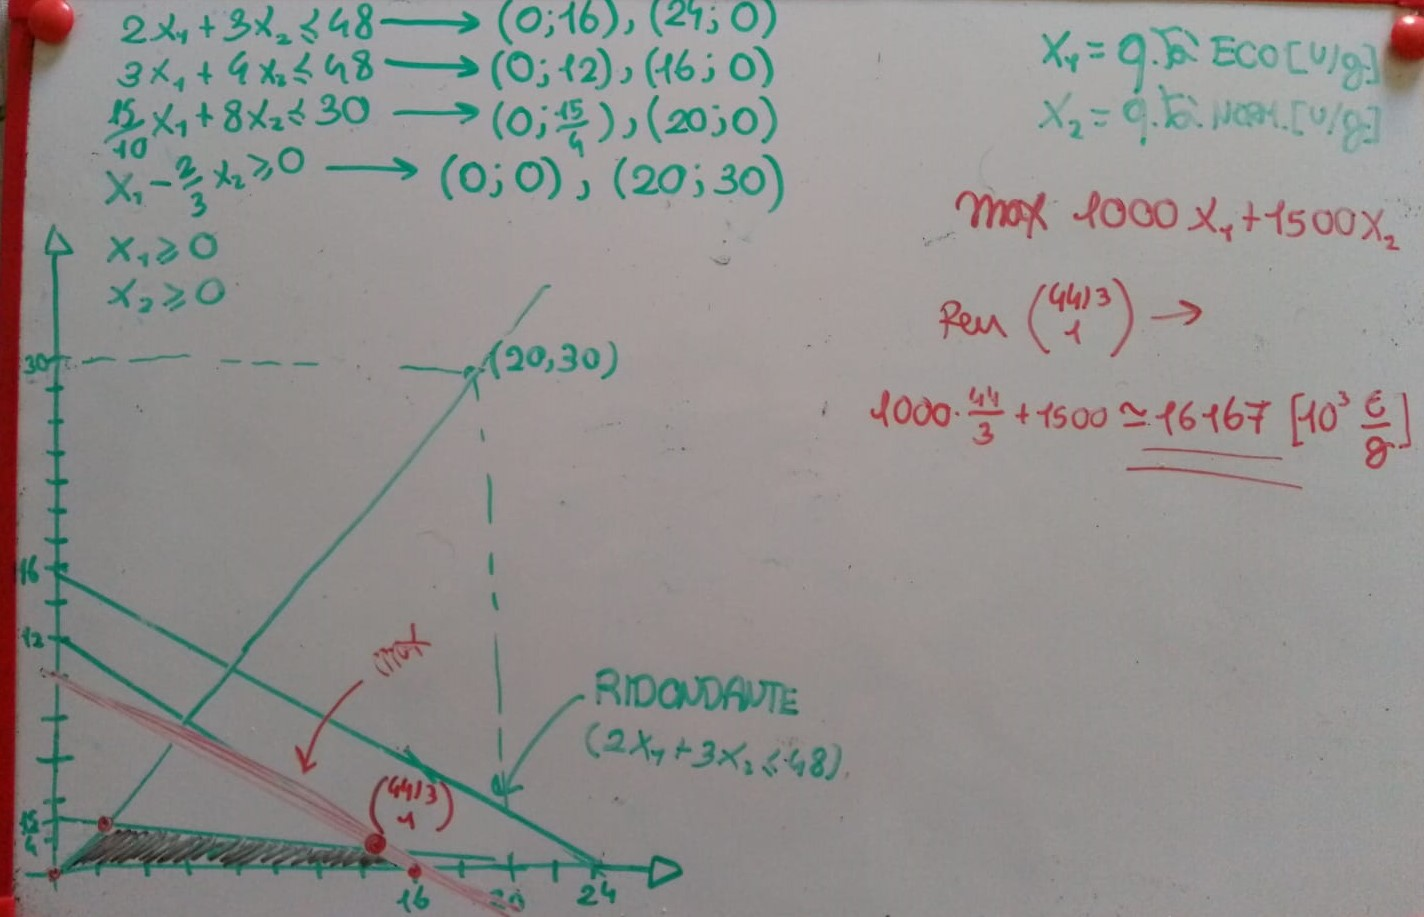
\includegraphics[scale=0.2]{esercizioauto.jpeg}
\end{figure}




\section{Esercizio 2:} sembra lo stesso di prima ma il modello matematico e decisionale è radicalmente diverso. Una azienza produce due diversi modelli di autovettura: Economica e Normale. Ogni autovettura è lavorata da uno qualunque di tre robot che operano in parallelo A, B e C. I tempi di lavorazione (in minuti per unità) sono riportati in tabella unitamente ai prezzi unitari di vendita (in migliaia di \euro).
\begin{table}[h!]
    \centering
    \begin{tabular}{|c|c|c|}
    \hline
     & Economica [m/u] & Normale [m/u]\\
    \hline
    \hline
    A & 20 & 30\\
    \hline
    B & 30 & 40\\
    \hline
    C & 15 & 80\\
    \hline
    prezzo [$10^3$ \euro] & 1000 & 1500\\
    \hline
    \end{tabular}
\end{table}
I robot A e B sono disponibili per 8 ore al giorno, mentre il robot C per 5 ore al giorno. Il numero di autovetture economiche prodotte deve costituire almeno il 40\% della produzione giornaliera complessiva. Formulare un problema di Pl che consenta di decidere le quantità (non necessariamente intere) da produrre giornalmente.

\vspace{1cm}


\noindent Cosa cambia rispetto all'esercizio di prima? I tre robot operano in parallelo, cioè un'auto è costruita da un robot soltanto, e non deve passare per tutti e tre i robot A,B e C in ordine. Quindi se prima graficamente avevamo una catena che, passando per A, B e poi C sfornava sia autovetture economiche che normali, adesso abbiamo il seguente grafico:
\begin{figure}[h!]
    \centering
    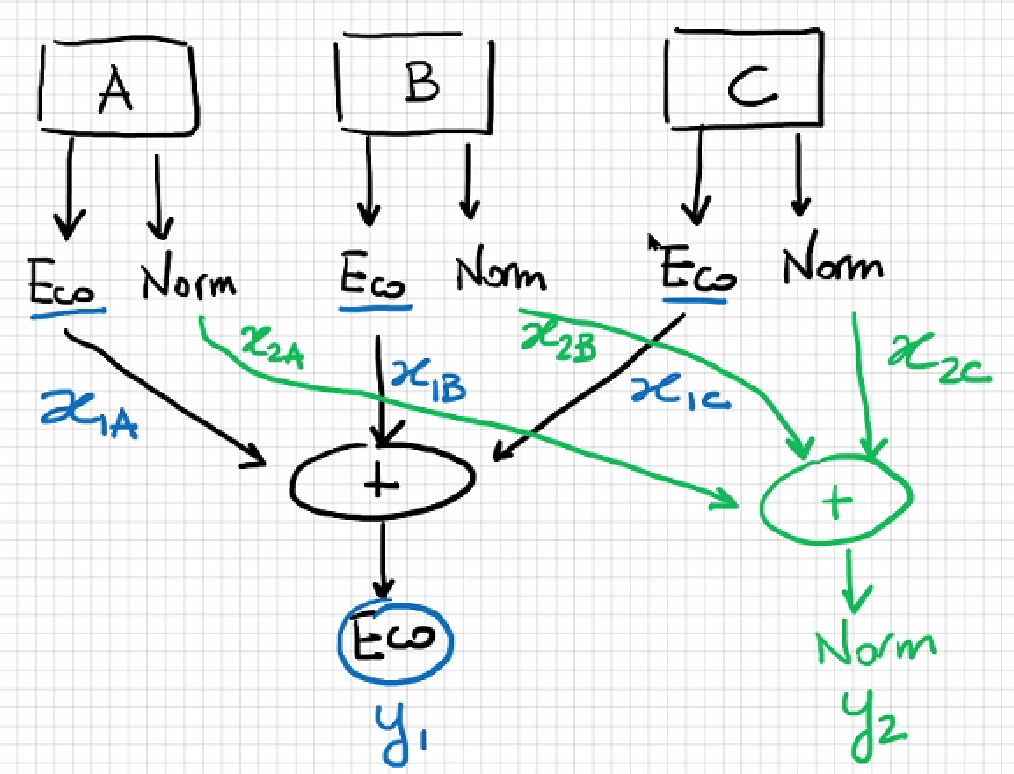
\includegraphics[scale=0.5]{esercizioauto2.png}
\end{figure}
Dove abbiamo definito le seguenti incognite:
\begin{itemize}
    \item $x_{1A}$: economiche prodotte giornalmente da A
    \item $x_{1B}$: economiche prodotte giornalmente da B
    \item $x_{1C}$: economiche prodotte giornalmente da C
    \item $x_{2A}$: normali prodotte giornalmente da A
    \item $x_{2B}$: normali prodotte giornalmente da B
    \item $x_{2C}$: normali prodotte giornalmente da C
    \item $y_1$: economiche prodotte giornalmente in totale
    \item $y_2$: normali prodotte giornalmente in totale
\end{itemize}
Notiamo che $y_1$ non è indipendente dalle altre variabili, non possiamo dargli un valore a caso, ma il suo valore è la somma di $x_{1A} + x_{2A} + x_{3A}$, analogo ragionamento per $y_2$. La funzione obiettivo è invece:
\begin{equation*}
    max 1000y_1 + 1500y_2
\end{equation*}
Vediamo ora i vincoli:
\begin{equation*}
    \text{per il robot A:} \hspace{1cm} 20x_{1A} + 30x_{2A} \leq 480
\end{equation*}
\begin{equation*}
    \text{per il robot B:} \hspace{1cm} 30x_{1A} + 40x_{2A} \leq 480
\end{equation*}
\begin{equation*}
    \text{per il robot C:} \hspace{1cm} 15x_{1A} + 80x_{2A} \leq 300
\end{equation*}
\begin{equation*}
    \text{per la quantità di economiche prodotte:} \hspace{1cm} y_1 \geq 40\%(y_1+y_2)
\end{equation*}
\begin{equation*}
    \text{vincoli di non negatività:} \hspace{1cm} x_{ij}, i = 1,2; j \in \{A,B,C\}
\end{equation*}
Sostituendo a $y_1$ e $y_2$ le variabili $x_{ij}$, il problema si mostra come un PL a 6 variabili, quindi di certo non graficabile sul piano. Il professore lo risolve con AMPL.


\newpage


\section{Esercizio 3:} Determinare tutti i vertici del poliedro P descritto dalle disuguaglianze e uguaglianze seguenti (in nero):
\begin{figure}[h!]
    \centering
    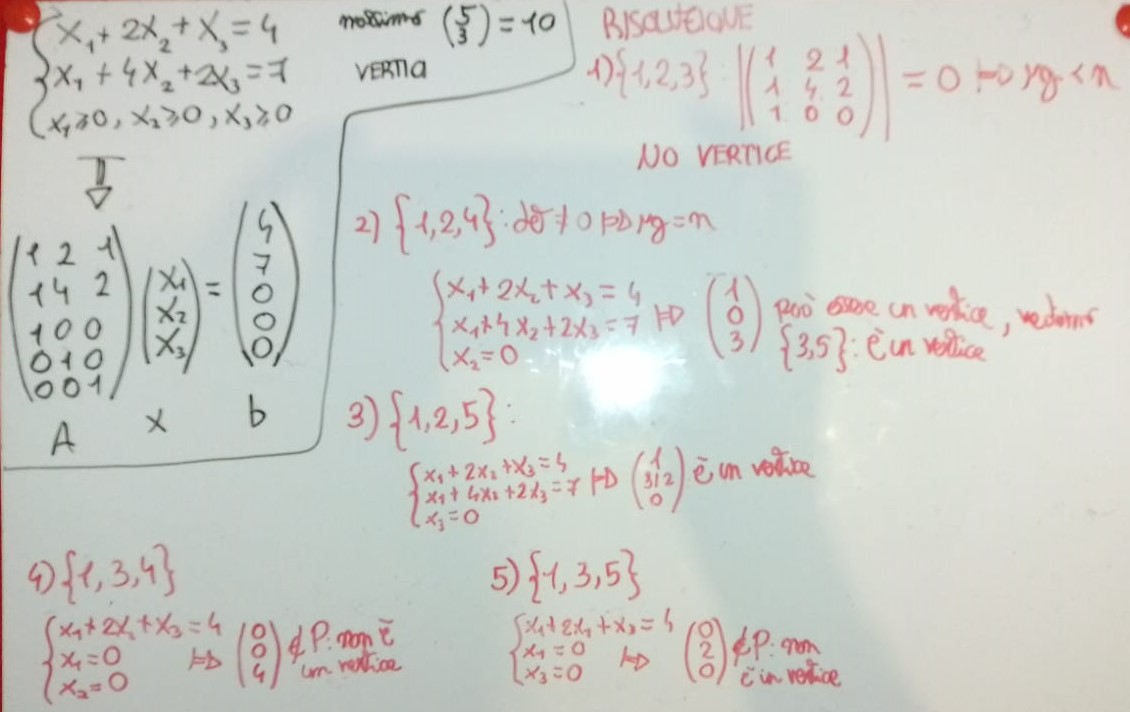
\includegraphics[scale=0.3]{esercizio3_1.jpeg}
\end{figure}
\begin{figure}[h!]
    \centering
    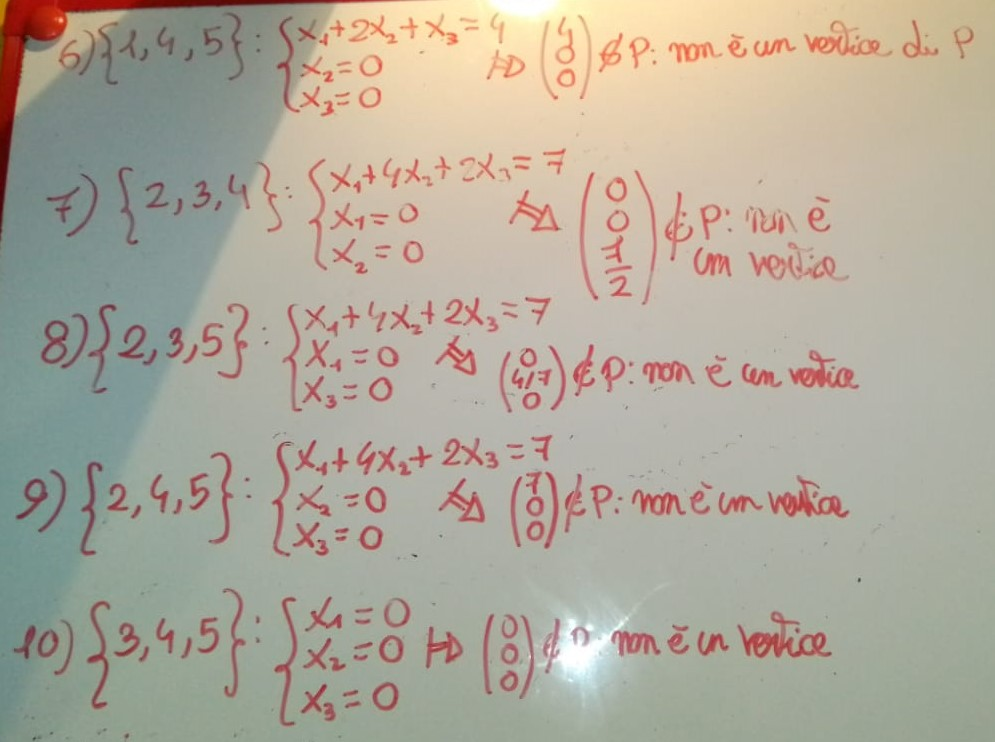
\includegraphics[scale=0.3]{esercizio3_2.jpeg}
\end{figure}



\newpage



\section{Secondo Risultato Veramente importante:} Il teorema fondamentale della programmazione lineare appoggia su questo risultato che facciamo oggi. Consideriamo:
\begin{equation*}
    P = \{x \in \mathbb{R}^n: Ax \geq b\}
\end{equation*}
con $A \in \mathbb{R}^{m \times n}$, b $\in \mathbb{R}^m$, $P \neq \varnothing$ e P che non contiene interamente rette (cioè non può avere un'intera retta dentro di sé). Allora P ammette almeno un vertice.

\paragraph{Dimostrazione:} Ricordiamo l'Ipotesi: 
\begin{equation*}
    P = \{x \in \mathbb{R}^n: Ax \geq b\}
\end{equation*}
Deve essere non vuoto (cioè deve esistere almeno un punto $\bar{x} \in P$) e non deve contenere interamente rette. Adesso sostituisco $\bar{x}$ nelle disuguaglianze così da costruire l'insieme I($\bar{x}$). Possono succedere due cose: 
\begin{itemize}
    \item Sono stato talmente bravo a scegliere $\bar{x}$, che:
    \begin{equation*}
        rg(a_i^T)_{i\in I(\bar{x})} = n
    \end{equation*}
    In tal caso $\bar{x}$ è un vertice. Ricordiamo che $(a_i^T)_{i\in I(\bar{x})}$ è la sottomatrice di A fatta dalle righe con indici dentro I$(\bar{x})$. 
    \item Caso più interessante e comune:
    \begin{equation*}
        rg(a_i^T)_{i\in I(\bar{x})} < n
    \end{equation*}
    In tal caso $\bar{x}$ non è un vertice
\end{itemize}
Adesso facciamo vedere costruttivamente come costruire un vertice. Per la dimostrazione che segue assumeremo che $\bar{x}$ non è un vertice.

\vspace{1cm} 

\noindent Se $\bar{x}$ non è un vertice allora:
\begin{equation*}
    a_i^Tx = 0 \hspace{1cm} i \in I(\bar{x})
\end{equation*}
Ammette infinite soluzioni oltre quella banale (se invece il rango è pieno ammette un'unica soluzione). Quindi sicuramente ammette una soluzione $d \in \mathbb{R}^n$, $d \neq 0$: $a_i^T d = 0$, $i \in I(\bar{x})$. Adesso abbiamo un punto $\bar{x}$ e una direzione d, che definiscono una retta. Che retta? Questa retta:
\begin{equation*}
    x(\lambda) = \bar{x} + \lambda d \hspace{1cm} \lambda \in \mathbb{R}
\end{equation*}
L'Ipotesi impone che questa retta non sia interamente dentro il poliedro. Immaginiamo di scoccare una freccia nella direzione di d, partendo in $\bar{x}$. Questa freccia si muoverà sulla semiretta corrispondente ai valori di $\lambda$ positivi. Questa freccia può fare due cose: o becca la frontiera del poliedro, la buca ed esce fuori (esce dalla zona ammissibile), oppure viaggia indefinitamente sempre all'interno del poliedro. Nel primo caso (caso favorevole), c'è un $\lambda > 0$ (non uguale a 0 perché $\bar{x}$ è nel poliedro) oltre il quale la semiretta esce dal poliedro. Nel secondo caso mi giro di 180 gradi e sparo un'altra freccia, in direzione -d quindi. Da quell'altra parte, per forza, la freccia deve bucare il poliedro e uscire. Perché se non fosse così vorrebbe dire che tutta la retta è contenuta nel poliedro e quindi non varrebbe l'Ipotesi. Da una delle due parti la retta deve incontrare la frontiera del poliedro, i punti sulla retta quindi sono ammissibili per un certo range di $\lambda$ e poi sono inammissibili. Poiché ci possiamo sempre girare di 180 gradi, quindi cambiando il segno a d, possiamo supporre WLOG che il lancio della freccia sia sempre per $\lambda > 0$. Rimanendo sempre in $i \in I(\bar{x})$, calcoliamo adesso:
\begin{equation*}
    a_i^Tx(\lambda) = a_i^T\bar{x} + \lambda a_i^T d 
\end{equation*}
$a_i^T\bar{x} = b_i$ perché $\bar{x}$ sta nel poliedro, mentre $a_i^T d = 0$ poiché abbiamo definito prima d come la soluzione dell'equazione $a_i^T x = 0$. Perciò:
\begin{equation*}
    a_i^Tx(\lambda) = b_i
\end{equation*}
Quindi, per $i \in I(\bar{x})$, i vincoli che sono soddisfatti all'uguaglianza da $\bar{x}$, continuano a essere soddisfatti all'uguaglianza da tutti i punti sulla retta. Siccome però non tutta la retta è nel poliedro, $\exists \bar{\lambda} > 0$ (che poniamo positivo proprio per quanto detto prima, poiché possiamo sempre cambiare direzione e passare a -d) t.c. quando $\lambda = \bar{\lambda}$ $\exists j \notin I(\bar{x})$ t.c. $a_j^T\bar{x} > b_j$, $a_j^Tx(\bar{\lambda}) = b_j$. Quindi un vincolo non attivo in $\bar{x}$, ma attivo in $x(\bar{\lambda})$. Quindi, per $0 < \lambda < \bar{\lambda}$ tale vincolo è soddisfatto (non all'uguaglianza), per $\lambda = \bar{\lambda}$ il vincolo diventa attivo, per $\lambda > \bar{\lambda}$ il vincolo diventa violato. Perciò per $\lambda > \bar{\lambda}$ la semiretta esce fuori dal poliedro, cioè dall'area ammissibile. Quindi, in $\bar{x}$ e su tutti gli altri punti della retta (anche $x(\bar{\lambda})$) sono attivi i vincoli $i \in I(\bar{x})$; in $x(\bar{\lambda})$ invece, ho un numero di vincoli attivi sicuramente più grande rispetto al numero di vincoli attivi in $\bar{x}$, almeno di uno: il vincolo $j \notin I(\bar{x})$ che abbiamo trovato prima. Quindi in $x(\bar{\lambda})$ ci sono più vincoli attivi. 


\vspace{1cm}

\noindent Adesso dobbiamo dimostrare che $a_j^T$ è linearmente indipendente da $(a_i^T)_{i \in I(\bar{x})}$. Perché ci interessa sta cosa? Perché se riusciamo a dimostrarlo, allora:
\begin{equation*}
    rg\left(\begin{pmatrix}
    a_i^T & i \in I(\bar{x})
    a_j^T
    \end{pmatrix}\right) > rg(a_i^T)_{i \in I(\bar{x})}
\end{equation*}
Cioè la matrice costruita prendendo le n righe solite $a_i^T$ $i \in I(\bar{x})$, e aggiungendo come ultima riga $a_j^T$ ha un rango maggiore di 1 rispetto al rango della nostra matrice $(a_i^T)_{i \in I(\bar{x})}$. Questo perché abbiamo detto che la matrice $(a_i^T)_{i \in I(\bar{x})}$ ha un rango minore di n, poiché $\bar{x}$ non è un vertice del poliedro. Quindi la nuova matrice con questa ultima riga ha sicuramente un rango maggiore di $(a_i^T)_{i \in I(\bar{x})}$, ma potrebbe comunque essere minore di n. Questo dobbiamo dimostrarlo per contraddizione: supponiamo $a_j^T$ è linearmente dipendente da $(a_i^T)_{i \in I(\bar{x})}$, vuol dire che posso scrivere il vettore $a_j$ come combinazione lineare dei vettori $a_i$ con $i \in I(\bar{x}$:
\begin{equation*}
    a_j = \sum_{i \in I(\bar{x})} \beta_i a_i
\end{equation*}
Quindi:
\begin{equation*}
    a_j^Tx(\bar{\lambda}) = \sum_{i \in I(\bar{x})} \beta_i a_i^T x(\bar{\lambda}) = \sum_{i \in I(\bar{x})} \beta_i b_i = b_j
\end{equation*}
Dove la seconda uguaglianza discende dal fatto che $a_i^Tx(\lambda) = b_i$ quando $i \in I(\bar{x})$, per tutta la retta, quindi anche in $\bar{\lambda}$. Mentre l'ultima equazione discende da $a_j^Tx(\bar{\lambda}) = b_j$, proprio per come abbiamo definito $x(\bar{\lambda})$. Adesso facciamo la stessa cosa per:
\begin{equation*}
    a_j^T\bar{x} = \sum_{i \in I(\bar{x})} \beta_i a_i^T\bar{x} = \sum_{i \in I(\bar{x})} \beta_i b_i > b_j
\end{equation*}
Dove la seconda uguaglianza discende per lo stesso motivo dell'espressione precedente, mentre l'ultima equazione discende da: $a_j^T\bar{x} > b_j$. Ma quindi:
\begin{equation*}
    \sum_{i \in I(\bar{x})} \beta_i b_i = b_j > b_j
\end{equation*}
E scadiamo in un assurdo $\square$

\vspace{1cm}

\noindent Ricapitolando: i vincoli attivi in $x(\bar{\lambda})$ sono almeno uno di più di quelli di $\bar{x}$, e la sottomatrice composta da  $(a_i^T)_{i \in I(\bar{x})}$ più $a_j^T$ cresce di uno di rango rispetto a $(a_i^T)_{i \in I(\bar{x})}$ da solo. Concettualmente adesso immaginiamo di \textit{ripetere} lo stesso procedimento da questo nuovo punto $x(\bar{\lambda})$, cioè diventa il nostro nuovo $\bar{x}$. Da questo punto cerchiamo il nuovo punto, cioè il nostro nuovo $x(\bar{\lambda})$. Otterremo così una nuova sottomatrice con il rango maggiore di 1 rispetto alla precedente. Ripetiamo il procedimento al più n-1 volte (nel caso in cui il rango della sottomatrice originaria fosse 1, sennò di meno di n-1), così da ottenere una sottomatrice di A con rango pari a n. Arrivati all'ultimo punto, quello la cui nuova riga farà diventare la nuova sottomatrice di rango n, \textit{esso è un vertice}, proprio perché il rango della sottomatrice è n: abbiamo quindi \textit{costruito un vertice}.
\begin{figure}[h!]
    \centering
    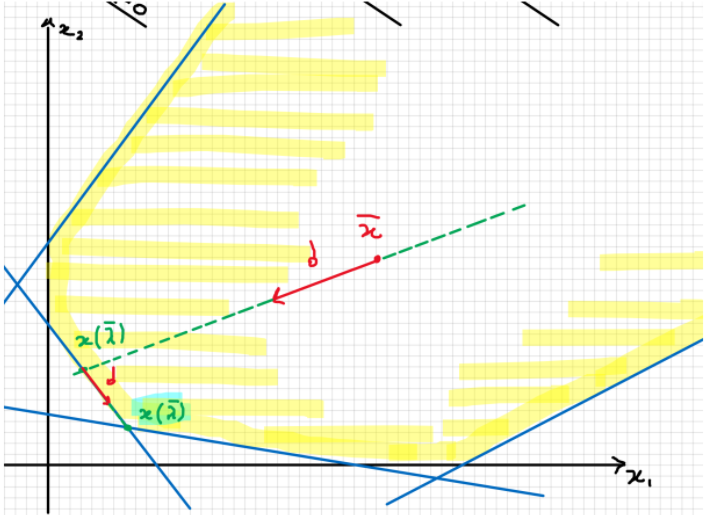
\includegraphics[scale=0.5]{costruzionevertice.png}
    \caption{Partiamo da $\bar{x}$, per cui il rango della matrice dei vincoli attivi è minore di n, quindi esiste una direzione d. Il punto $\bar{x}$ e la direzione d (che, dato che non deve essere soluzione di nessuna equazione, poiché non ci sono vincoli attivi, può essere scelta a caso) definiscono una retta (quella tratteggiata). Per $\lambda$ sufficientemente grandi la retta buca il poliedro; il punto in cui buca è proprio x($\bar{\lambda}$). Vediamo che all'inizio in $\bar{x}$ non ci sono vincoli attivi (cioè $\bar{x}$ non è poggiato su nessuna retta), mentre nel punto che raggiungiamo, cioè $x(\bar{\lambda})$, ce n'è 1 (perché il punto è poggiato su una sola retta). Potevamo anche atterrare su un $x(\bar{\lambda})$ che aveva più di un vincolo attivo (tipo se d fosse stata rivolta più verso il basso avremmo potuto prendere quel punto all'incrocio tra una delle rette e l'asse x, e lì ci sarebbero stati due vincoli attivi, proprio perché il punto sarebbe stato poggiato su due rette, all'intersezione. Comunque, proprio perché non siamo atterrati in un punto con più vincoli attivi, il rango non è ancora n, e dobbiamo riprovare: $x(\bar{\lambda})$ diventa il nostro nuovo $\bar{x}$, stavolta ho un vincolo attivo da rispettare, quindi la mia direzione non può essere presa a caso, ma deve essere identificata sulla retta di appartenenza di $x(\bar{\lambda})$ (perché d deve essere soluzione di un'equazione dei vincoli attivi, quindi non posso prendere le sue componenti a caso), proprio perché deve rispettare il suo vincolo attivo. Con il mio punto e la mia direzione mi dirigo verso il basso e trovo il mio nuovo $x'(\bar{\lambda})$, e questo, possiamo vedere dal grafico, che è un vertice. Cioè è un punto t.c. la sottomatrice con la riga in più ha rango pari ad n. Vogliamo fare un'altra metafora? Pensa di essere in una stanza bendato, cammini fino al muro, ci sbatti contro, quel punto è il tuo $x(\bar{\lambda})$. Da lì inizi a muoverti di nuovo, questa volta non a caso ma seguendo la linea del muro, finché non incontri uno spigolo: quello sarà il tuo vertice.}
\end{figure}
Siamo quindi riusciti a costruire un vertice da un poliedro che rispetta le Ipotesi date all'inizio. Quindi abbiamo dimostrato che un poliedro che rispetta quelle Ipotesi ammette almeno un vertice $\square$

\vspace{1cm}

\noindent Adesso tocca all'implicazione inversa, cioè dobbiamo dimostrare che: consideriamo
\begin{equation*}
    P = \{x \in \mathbb{R}^n: Ax \geq b\}
\end{equation*}
e supponiamo che P ammetta almeno un vertice $\bar{x} \in P$. Allora P non contiene rette.

\paragraph{Dimostrazione (per assurdo):} stavolta non necessitiamo di assumere che il poliedro sia diverso dall'insieme vuoto, perché esiste un punto che è un vertice (quindi almeno quel punto ce l'ha, e quindi non è vuoto). Ricordiamoci che se $\bar{x}$ è vertice allora rg($a_i^T)_{i \in I(\bar{x})}$ = n. Bene, ora dimostriamo per assurdo, quindi supponiamo che:
\begin{equation*}
    \bar{x} \hspace{0.2cm} \text{è vertice} \implies \hspace{0.2cm} \text{P contiene una retta}
\end{equation*}
Cioè $\exists x \in P$, $d \neq 0$ t.c. $x(\lambda) = x + \lambda d \in P$ $\forall \lambda \in \mathbb{R}$. Quindi per tutti i $\lambda$. Consideriamo che d non l'abbiamo calcolata nel solito modo questa volta, perché il rango è massimo, quindi la soluzione del sistema è unica, bensì l'abbiamo trovata in un qualsiasi altro modo. Proprio perché il rango è massimo e $d \neq 0$ non è soluzione del sistema, vale:
\begin{equation*}
    a_i^Td \neq 0
\end{equation*}
Bene, ora possiamo calcolare:
\begin{equation*}
    a_i^Tx(\lambda) = a_i^Tx + \lambda a_i^Td
\end{equation*}
Con $a_i^Tx \geq b_i$, poiché x è ammissibile (dato che appartiene al poliedro), e $a_i^Td$ appena calcolato $\neq$ 0. Quindi adesso abbiamo diversi casi possibili:
\begin{itemize}
    \item $a_i^Td > 0$, se $\lambda > 0$ allora $a_i^Tx(\lambda) = a_i^Tx + \lambda a_i^Td > b_i$, se invece $\lambda < 0$ esisteranno dei valori di $\lambda$ per cui $a_i^Tx(\lambda) = a_i^Tx + \lambda a_i^Td < b_i$. Quindi esiste almeno un lambda negativo per cui $a_i^Tx(\lambda)$ non è ammissibile (perché $< b_i$). Ma abbiamo detto che tutta la retta era ammissibile, quindi non ci possono essere punti $< b_i$. Allora significa che $a_i^T d$ non può essere $> 0$.
    \item Ci rimane solo $a_i^T d < 0$ allora. Ma ragionando specularmente rispetto al punto sopra vediamo che si ribaltano le cose: per $\lambda < 0$ si ha che $a_i^Tx(\lambda) > b_i$, ma per almeno un $\lambda > 0$ esiste un punto non ammissibile $a_i^Tx(\lambda) < b_i$. Ma abbiamo detto che tutta la retta era ammissibile. Quindi $a_i^Td$ non può essere neanche $< 0$
\end{itemize}
Ma quindi $a_i^Td$ non deve essere uguale a 0, né maggiore di 0, né minore di 0: ASSURDO!!! Questo ragionamento lo ripetiamo per tutte le $i \in I(\bar{x})$. Ma non è finita: ok quindi siamo obbligati a cambiare idea, per forza di cose $a_i^Td$ deve essere uguale a 0, è l'unico modo di far funzionare la cosa. Quindi se $a_i^T d = 0$, $\forall i \in I(\bar{x})$, con $d \neq 0$, significa che esiste una soluzione diversa da quella banale per il sistema, cioè il rango non è massimo:
\begin{equation*}
    rg(a_i^T)_{i \in I(\bar{x})} < n
\end{equation*}
Ma questo è ASSURDO! Perché abbiamo supposto all'inizio che $\bar{x}$ fosse un vertice, e che quindi il rango fosse n! $\square$

\vspace{1cm}

\noindent Questo risultato implica che: se considero P poliedro, fatto in qualsiasi modo, intersecato, per esempio, con il poliedro $\{x in \mathbb{R}^n: x \geq 0\}$, e chiamo questa inserserzione P', cosa può succedere?
\begin{itemize}
    \item P' = $\varnothing$
    \item P' $\neq \varnothing$ non contiene rette, perché solo per $x \geq 0$ non si può definire una retta tutta contenuta. Questo significa, per quanto appena trovato, che ha almeno un vertice. 
\end{itemize} 
Per fare un altro esempio di ciò: riprendiamo l'esercizio 3 fatto prima, vediamo che la zona ammissibile è un poliedro intersezione delle prime due rette e del quadrante positivo in tre dimensioni ($x_1,x_2,x_3 \geq 0)$. Per lo stesso discorso fatto ora, non può contenere rette, e quindi ha almeno un vertice, come abbiamo già visto. Questa è una caratterizzazione dei poliedri non vuoti quindi.



\section{Un altro esercizio sui Vertici:} 

\begin{figure}[h!]
    \centering
    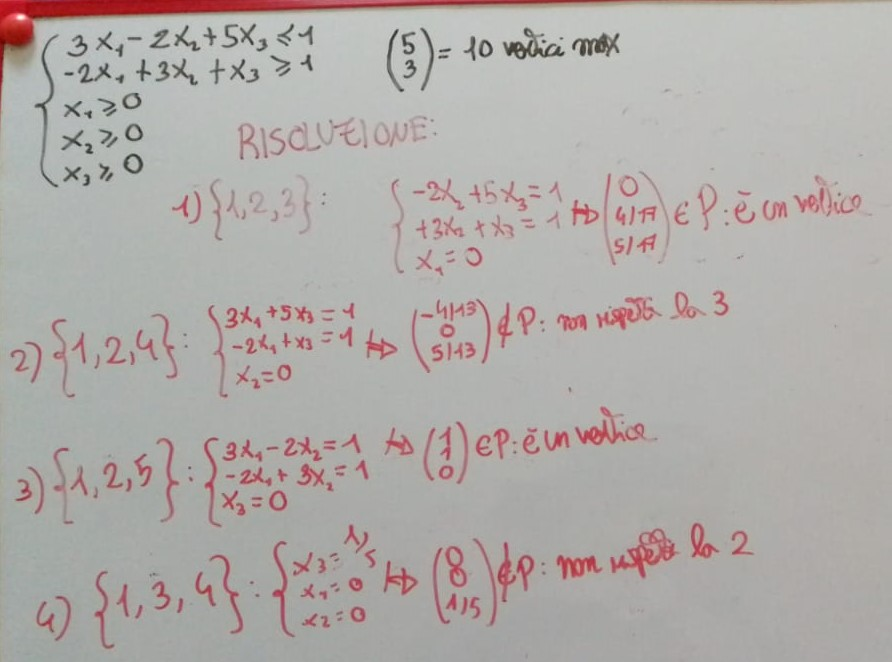
\includegraphics[scale=0.3]{EsercizioVerticiAncora.jpeg}
\end{figure}
Facciamo solo quattro vertici su 10 perché gli altri sono uguali.



\section{Altri esercizi:}

\paragraph{1. Dire quali delle seguenti affermazioni sono corrette.}
\begin{itemize}
    
    \item[(a)] In $\mathbb{R}^3$, l'intersezione tra una sfera centrata nell'origine di raggio 1 e l'ortante positivo\footnote{Un ortante è una delle otto regioni di spazio in cui è diviso lo spazio tridimensionale. L'ortante positivo è quindi quello in cui tutte e tre le variabili assumono valori positivi. Il concetto di ortante è analogo al concetto di quadrante nel piano} è un politopo?
    
    \subparagraph{Risposta:} stiamo parlando del seguente oggetto:
    \begin{equation*}
        D = \{x \in \mathbb{R}^3: x_1^2 + x_2^2 + x_3^2 \leq 1\} \cap \{x_1 \geq 0, x_2 \geq 0, x_3 \geq 0\}
    \end{equation*}
    Ma il primo insieme dell'intersezione non è un semispazio! Poiché presenta dei termini quadratici (quindi non lineari), e quindi \textit{non rappresenta un semispazio}. Non stiamo quindi parlando di intersezione tra semispazi e iperpiani, e quindi D non è un poliedro, tantomeno un politopo.
    
    
    \item[(b)] In $\mathbb{R}^2$, l'insieme dei punti a coordinate intere del primo quadrante è un insieme convesso?
    
    \subparagraph{Risposta:} facciamo un grafico dei punti a coordinate intere del primo quadrante di $\mathbb{R}^2$
    \begin{figure}[h!]
        \centering
        \includegraphics{puntiinteriprimoquadrantepiano}
    \end{figure}
    Vediamo dal grafico che il segmento passa per tutti i punti in mezzo ai due scelti, ma solo questi ultimi, che sono gli estremi, sono compresi nel nostro insieme: tutti gli altri punti in mezzo non fanno parte dell'insieme. Quindi no: in $\mathbb{R}^2$, l'insieme dei punti a coordinate intere del primo quadrante NON è un insieme convesso.
    
    \item[(c)] Dati $y \in \mathbb{R}^n$ e $z \in \mathbb{R}^n$, l'insieme \{$x \in \mathbb{R}^n: x = \lambda y + (1 - \lambda)z, 0 \leq \lambda \leq \frac{1}{2}$\} è un insieme convesso?
    
    \subparagraph{Risposta:} Sì! Anche se $\lambda \in [0, \frac{1}{2}]$ e non $\lambda \in [0,1]$, comunque si sta parlando di un segmento, precisamente un sottosegmento di quello dato nella domanda. Comunque, essendo un segmento, è un insieme convesso.
    
    
    \item[(d)] L'insieme \{$x \in \mathbb{R}^n: Ax \geq b, l \leq x \leq u$\}, con A matrice m $\times$ n, x $\in \mathbb{R}^n$, $b \in \mathbb{R}^m$, l $\in \mathbb{R}^n$, u $\in \mathbb{R}^n$ è un politopo.
    
    \subparagraph{Risposta:} sì! Si tratta di un politopo perché la prima condizione $Ax \geq b$ rivela un semispazio, mentre la seconda $l \leq x \leq u$ impone che di questo semispazio venga presa solo una zona limitata, e un poliedro limitato è un politopo. Vediamo in $\mathbb{R}^2$:
    \begin{figure}[h!]
        \centering
        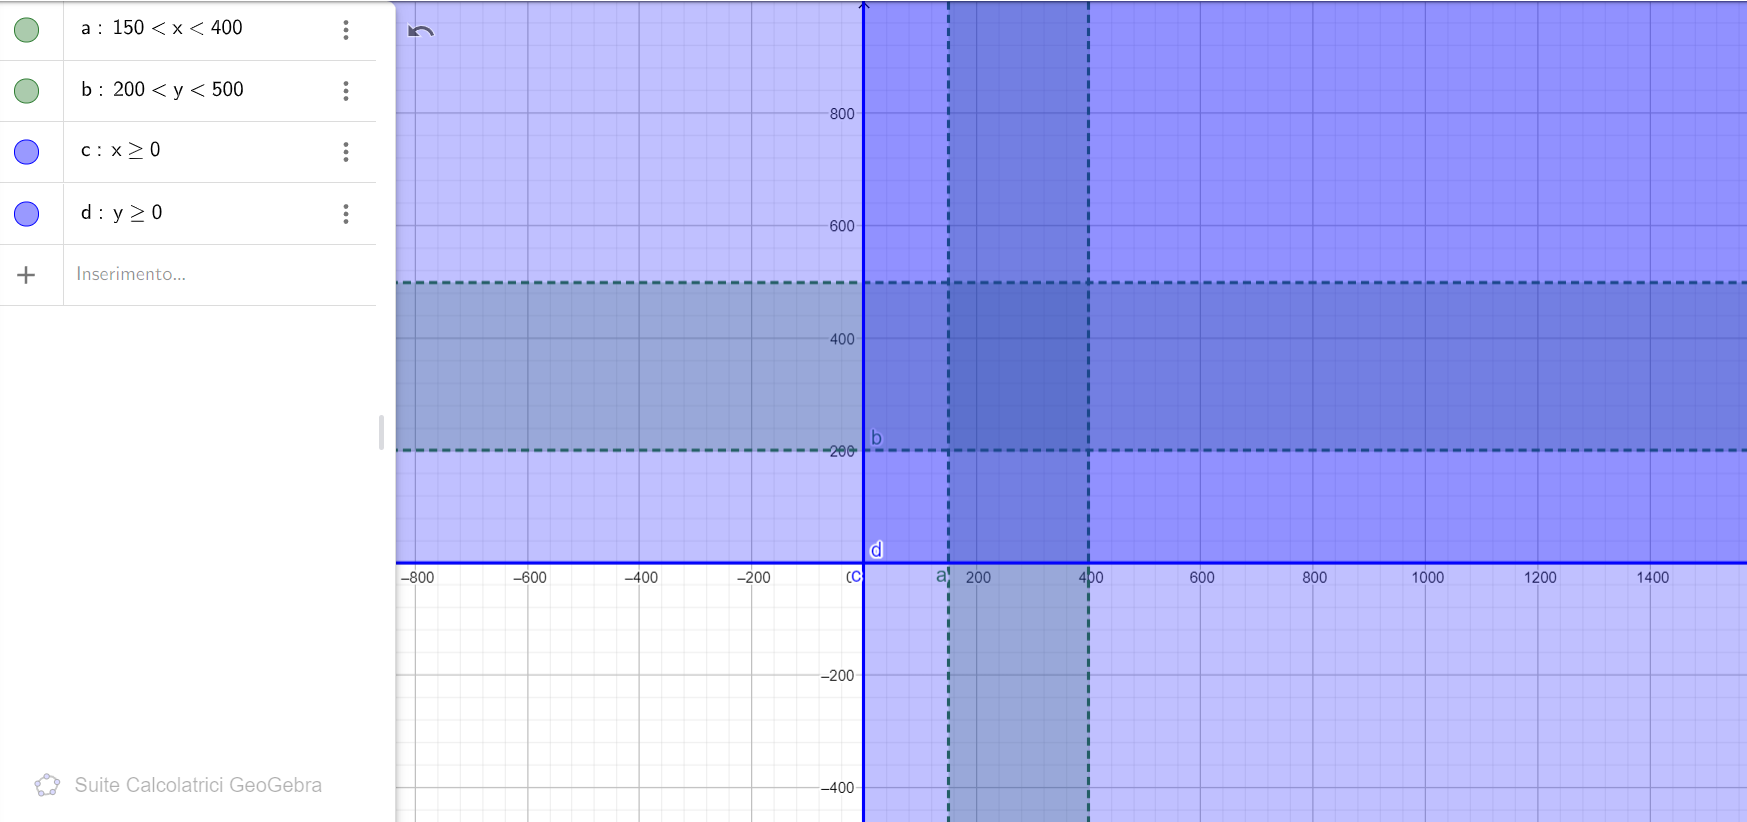
\includegraphics[scale=0.3]{geogebrapolitopi.png}
    \end{figure}
    Vediamo in blu scuro il semispazio determinato dalla prima condizione, mentre in verde scuro la zona determinata dalla seconda condizione. L'intersezione dei due è chiaramente un insieme limitato.
\end{itemize}


\paragraph{2. Si consideri il poliedro descritto dal seguente sistema:}
\begin{equation*}
    x_1 + 2x_2 + x_3 = 4
\end{equation*}
\begin{equation*}
    x_1 + 4x_2 + 2x_3 = 7
\end{equation*}
\begin{equation*}
    2x_1 + 10x_2 + 5x_3 + x_4 = 17
\end{equation*}
\begin{equation*}
    x_i \geq 0, i = i, ..., 4
\end{equation*}
Dire quali delle seguenti affermazioni sono corrette:
\begin{itemize}
    \item[(a)] Il punto $(1, 1, 1, 0)^T$ è vertice del poliedro?
    
    \subparagraph{Risposta:} Per verificarlo innanzitutto dobbiamo vedere se il punto appartiene all'insieme. Appartiene, perché rispetta tutte e 7 le disuguaglianze. Ora dobbiamo trovare n = 4 disuguaglianze soddisfatte all'uguaglianza, così da formare l'insieme dei vincoli attivi I($(1, 1, 1, 0)^T$). Troviamo le seguenti righe della matrice che corrispondono a vincoli attivi:
    \begin{equation*}
        I((1, 1, 1, 0)^T) = \{1,2,3,7\}
    \end{equation*}
    Poiché ci sono n = 4 vincoli attivi andiamo avanti, ma ancora non possiamo dire se è un vertice. Dobbiamo scrivere la sottomatrice individuata da questi indici e verificare che abbia rango uguale a 4.
    \begin{equation*}
        \begin{pmatrix}
            1 & 2 & 1 & 0\\
            1 & 4 & 2 & 0\\
            2 & 10 & 5 & 1\\
            0 & 0 & 0 & 1
        \end{pmatrix}
    \end{equation*}
    Lo sviluppo di Laplace ci porta a dire che il determinante è 0, quindi la matrice non ha rango 4 (notare che potevamo vederlo già dal fatto che la seconda e la terza colonna sono dipendenti). Quindi $(1,1,1,0)^T$ non è un vertice.
    
    
    \item[(b)] Il punto $(1, 1, 1, 1)^T$ è vertice del poliedro? No, sostituendo i punti nella terza equazione troviamo un vincolo violato, quindi il punto è proprio inammissibile.
    
    
    \item[(c)] L'origine degli assi è vertice del poliedro? No, sostituendo i punti in una qualunque delle uguaglianze vediamo che sono vincoli violati, quindi il punto è proprio inammissibile.
    
    
    \item[(d)] Il poliedro non ammette vertici perché il numero delle variabili presenti (n) è maggiore del numero di vincoli di uguaglianza (m). Non c'entra proprio niente, è una frase matta. I vertici andrebbero calcolati magari qualcuno ce n'è (vedendo che al massimo possono essere $\binom{7}{4} = 35$.
\end{itemize}



\section{Esercizio 1:} Consideriamo il seguente problema di PL
\begin{equation*}
    min -x_1 - 2x_2 - x_3
\end{equation*}
\begin{equation*}
    c.v. x_1 + 2x_2 + x_3 \leq 3
\end{equation*}
\begin{equation*}
    3x_1 - x_2 + x_3 \leq 2
\end{equation*}
\begin{equation*}
    2x_1 ++ x_2 + x_3 \leq 3
\end{equation*}
\begin{equation*}
    4x_1 + x_2 - 2x_3 \leq 4
\end{equation*}
supponiamo che NON sia illimitato inferiormente (il prof lo ha verificato). Quindi se è limitato inferiormente potrebbe succedere che è non ammissibile (S $\neq \varnothing$) o che ammette soluzione ottima (esiste una $x^* \in S $ t.c. $f(x^*) < f(x)$ per ogni x $\in$ S). Vediamo che il problema è ammissibile (sarebbe stato non ammissibile se ci fosse neanche una soluzione che rispettasse tutti i vincoli, ma banalmente la soluzione di tutti 0 è ammissibile). Ciò vuol dire che il problema, che è limitato inferiormente, non può essere non ammissibile: ammette quindi soluzione ottima. Abbiamo detto che E = $\begin{pmatrix}
    0\\
    0\\
    0
\end{pmatrix} \in P$. Con P $\in \mathbb{R}^3$ poliedro del problema. Noi comunque non siamo ancora al livello di poter trovare la soluzione ottima, quindi non lo vogliamo fare, noi vogliamo innanzitutto fare un Anamnesi di E. Vedere ad esempio quanti vincoli sono attivi in E:
\begin{equation*}
    I(E) = \varnothing
\end{equation*}
Ciò vuol dire che il punto E è ammissibile ma non è un vertice. Bene, ora, a partire da E, vogliamo trovare un punto ammissibile che rende però attivo almeno un vincolo. Questo lo facciamo con il procedimento che abbiamo fatto per la dimostrazione del teorema scorso. Facendo questa procedura, dobbiamo però assicurarci di trovare un punto che non peggiori la funzione obiettivo. Quindi innanzitutto dobbiamo calcolare quanto vale la funzione obiettivo in E:
\begin{equation*}
    c^TE = 0
\end{equation*}
Dove con c si indica il vettore dei coefficienti della funzione obiettivo, cioè $\begin{pmatrix}
    -1\\
    -2\\
    -1
\end{pmatrix}$. Quindi il nostro obiettivo è trovare un punto ammissibile, con un vincolo attivo in più e che calcolandoci la funzione obiettivo dia un valore minore o al più uguale a 0. Ripassiamo la procedura per trovare un punto con più vincoli attivi a partire da un altro: troveremo questo punto su una semiretta che ha origine dal punto E e ha una certa direzione d. Quest'ultima, la direzione d, la troviamo come soluzione di un particolare sistema omogeneo: il sistema in cui considero le righe della matrice dei coefficienti dei vincoli (che avevamo chiamato A)
\begin{equation*}
    a_i^Td = 0 \hspace{1cm} i \in I(E) \neq \varnothing
\end{equation*}
Cioè ho un'equazione come quella di sopra per ogni $i \in I(E)$, ma non ci sono i dentro I(E), quindi non ci sono equazioni che d deve soddisfare. Quindi, poiché non deve soddisfare nessuna equazione, può essere una qualunque direzione d (quindi la retta può puntare ovunque, mentre quando si hanno dei vincoli, la d dovrà per forza di cose rispettarli e quindi non potrà scegliere a caso dove direzionarsi), ovviamente tranne la nulla che non è una direzione. Ok prendiamo allora:
\begin{equation*}
    \bar{d} = \begin{pmatrix}
        1\\
        0\\
        0
    \end{pmatrix}
\end{equation*}
Adesso abbiamo il punto E e la direzione $\bar{d}$, ci serve la semiretta: x($\lambda$) = E + $\lambda$d. Adesso calcoliamo la funzione obiettivo in $\bar{d}$, spiegheremo poi a cosa serve questo calcolo:
\begin{equation*}
    c^T\bar{d} = -1 < 0
\end{equation*}
Perché ci interessa questo? Proviamo a calcolare la funzione obiettivo nel punto parametrico $x(\lambda)$:
\begin{equation*}
    c^Tx(\lambda) = c^TE + \lambda c^T\bar{d} = 0 - \lambda
\end{equation*}
vediami quindi che sulla semiretta $x(\lambda)$ per $\lambda \in [0, \infty)$, la funzione obiettivo assume il valore 0 nel punto E (quindi per $\lambda = 0$) e valori strettamente negativi pari a $-\lambda$ su tutto il resto della semiretta. Quindi appena mi sposto da E lungo la semiretta positiva, ottengo punti che \textit{migliorano la funzione obiettivo}, perché sono minori di 0, come cercavamo. Ok però ci servono punti ammissibili e con più vincoli attivi di E. Allora che facciamo: cerchiamo di determinare il range di valori di $\lambda$ che ci permettono, sulla semiretta, di rimanere dentro al poliedro, e non violare nessun vincolo, quindi di essere ammissibili. Come facciamo? Determiniamo innanzitutto il vettore $x(\lambda)$:
\begin{equation*}
    x(\lambda) = E + \lambda d = \begin{pmatrix}
        0\\
        0\\
        0
    \end{pmatrix} + \lambda \begin{pmatrix}
        1\\
        0\\
        0
    \end{pmatrix} = \begin{pmatrix}
        \lambda\\
        0\\
        0
    \end{pmatrix}
\end{equation*}
Cosa facciamo? Sostituiamo il vettore $x(\lambda)$ nei vincoli che definiscono il poliedro, e otteniamo le seguenti disuguaglianze:
\begin{equation*}
    \lambda \leq 3
\end{equation*}
\begin{equation*}
    \lambda \leq \frac{2}{3}
\end{equation*}
\begin{equation*}
    \lambda \leq \frac{3}{2}
\end{equation*}
\begin{equation*}
    \lambda \leq 1
\end{equation*}
Quindi, affinché il punto $x(\lambda)$ sia ammissibile deve valere $\lambda \in [0,\frac{2}{3}]$. Ora che facciamo, prendiamo proprio:
\begin{equation*}
    x(\frac{2}{3}) = \begin{pmatrix}
        \frac{2}{3}\\
        0\\
        0
    \end{pmatrix} = B
\end{equation*}
Lo chiamiamo B. Calcoliamo la funzione obiettivo su B:
\begin{equation*}
    c^TB = -\frac{2}{3} < 0
\end{equation*}
Mh, ok, adesso allora prendiamo B e sostuiamolo nei vincoli, cercando quali e quante sono soddisfatte \textit{all'uguaglianza}.
\begin{equation*}
    I(B) = \{2\}
\end{equation*}
Nel punto E non c'erano vincoli attivi, nel punto B generato ce n'è uno. Il punto inoltre migliora la funzione obiettivo ed è ammissibile, quindi abbiamo fatto progressi. Adesso, ripartiamo da capo: il nostro E diventa il nostro punto B. Ora dobbiamo considerare il sistema omogeneo associato alla matrice che otteniamo con le righe della matrice A che sono dentro I(B). Stavolta I(B) non è vuoto, ma il sistema ha un'equazione:
\begin{equation*}
    a_2^Td = 0 \implies 3d_1 - d_2 + d_3 = 0
\end{equation*}
Vogliamo una soluzione diversa da quella nulla. Fissiamo $d_1$ e $d_2$ come parametri e otteniamo $d_2$ con cui prendiamo, ad esempio, $\bar{d} = \begin{pmatrix}
    0\\
    1
    1
\end{pmatrix}$. Quindi prendiamo la nostra retta parametrizzata:
\begin{equation*}
    x(\lambda) = B + \lambda \bar{d}
\end{equation*}
E come prima ci calcoliamo:
\begin{equation*}
    c^T\bar{d} = -3 < 0
\end{equation*}
E come prima, ancora:
\begin{equation*}
    c^Tx(\lambda) = c^TB - 3\lambda = -\frac{2}{3} - 3 < - \frac{2}{3}
\end{equation*}
Sempre prendendo la semiretta positiva con $\lambda > 0$. Quindi abbiamo ottenuto una retta i cui punti dopo B migliorano ancora di più la funzione obiettivo, perché assumono valori più piccoli di quello che viene assunto in B, punto iniziale della semiretta.



Avendo supposto che il problema sia limitato inferiormente, se tutta la semiretta fosse contenuta nel poliedro per ogni $\lambda > 0$, vuol dire che lungo la semiretta il valore della funzione obiettivo decresce infinitamente, ma il problema sarebbe illimitato. Quindi la semiretta non può stare tutta nel poliedro. Quindi a un certo punto la semiretta buca il poliedro e non è più contenuta. Ok, calcoliamoci il vettore parametrico della retta:
\begin{equation*}
    x(\lambda) = \begin{pmatrix}
        \frac{2}{3}\\
        0\\\
        0
    \end{pmatrix} + \begin{pmatrix}
        0\\
        \lambda\\
        \lambda
    \end{pmatrix} = \begin{pmatrix}
        \frac{2}{3}\\
        \lambda\\
        \lambda
    \end{pmatrix}
\end{equation*}
Ora sostiuiamo il punto nei vincoli per vedere fino a dove la semiretta ha punti ammissibili e non buca il poliedro:
\begin{equation*}
    \lambda \leq \frac{7}{9}
\end{equation*}
\begin{equation*}
    2 \leq 2
\end{equation*}
Cioè è soddisfatta sempre, per qualunque valore di $\lambda$ (ce lo dovevamo aspettare, si tratta del vincolo che B rispetta all'uguaglianza)
\begin{equation*}
    \lambda \leq \frac{5}{6}
\end{equation*}
\begin{equation*}
    \lambda \leq \frac{4}{9}
\end{equation*}
Quindi per $\lambda \in [0,\frac{4}{9}]$, $x(\lambda)$ è ammissibile. Come prima, prendiamo $\frac{4}{9}$:
\begin{equation*}
    x(\frac{4}{9}) = \begin{pmatrix}
        \frac{2}{3}\\
        \frac{4}{9}\\
        \frac{4}{9}
    \end{pmatrix} = C
\end{equation*}
E lo chiamiamo C, il nostro nuovo punto. Vediamo quanto vale la nostra funzione obiettivo:
\begin{equation*}
    c^TC = -\frac{2}{3}-\frac{8}{9}-\frac{4}{9} = -2
\end{equation*}
Quindi abbiamo generato un punto ammissibile che migliora ancora di più la funzione obiettivo. Adesso sostiuiamo il punto nelle disuguaglianze, così da vedere quanti vincoli rispetta all'uguaglianza. Si scopre che:
\begin{equation*}
    I(C) = \{2,4\}
\end{equation*}
Ovviamente il secondo vincolo era attivo, lo era già anche con B. Quindi abbiamo generato un punto C migliore di B. Continuiamo così, prendendo C come punto base stavolta. Prendiamo il sistema omogeneo che otteniamo considerando le righe della matrice A che hanno indice in I(C):
\begin{equation*}
    a_2^Td = 0 \implies 3d_1 - d_2 + d_3 = 0
\end{equation*}
\begin{equation*}
    a_4^Td = 0 \implies 4d_1 + d_2 + 2d_3 = 0
\end{equation*}
Da questo sistema, prendendo come parametro $d_3$, troviamo per esempio:
\begin{equation*}
    \bar{d} = \begin{pmatrix}
        -\frac{3}{7}\\
        -\frac{2}{7}\\
        1
    \end{pmatrix}
\end{equation*}
Quindi con C e $\bar{d}$ definiamo una retta, di cui prendiamo la semiretta positiva per lambda positivi:
\begin{equation*}
    x(\lambda) = C + \lambda \bar{d}
\end{equation*}
Questa direzione però è particolare, infatti:
\begin{equation*}
    c^T\bar{d} = 0
\end{equation*}
Quindi, poiché si tratta di un prodotto scalare, $\bar{d}$ ha direzione ortogonale al vettore che ha come componenti i coefficienti della funzione obiettivo. Questo è un problema, perché quando vado a calcolare:
\begin{equation*}
    c^Tx(\lambda) = c^TC
\end{equation*}
Ciò significa che su tutta la semiretta il valore della funzione obiettivo non cambia, è uguale a quanto vale in C, cioè -2. Però comunque sepoffa, l'importante è che non diventa peggiore di C, se permane costante ci sta bene. ATTENZIONE QUI: mentre prima potevamo dire con certezza che non tutta la semiretta fosse contenuta (perché la semiretta era "in discesa" e il problema si è assunto limitato inferiormente) adesso non possiamo dirlo con certezza, perché la funzione rimane costante e non diminuisce. Bisogna quindi provare a sostuituire questi punti nei vincoli e vedere se la semiretta è tutta contenuta oppure no. Facciamo un tentativo e vediamo. I punti parametrici sono:
\begin{equation*}
    x(\lambda) = \begin{pmatrix}
        \frac{2}{3}\\
        \frac{4}{9}\\
        \frac{4}{9}
    \end{pmatrix} + \begin{pmatrix}
        -\frac{3}{7}\lambda\\
        -\frac{2}{7}\lambda\\
        \lambda 
    \end{pmatrix} = \begin{pmatrix}
        \frac{2}{3}-\frac{3}{7}\lambda\\
        \frac{4}{9}-\frac{2}{7}\lambda\\
        \frac{4}{9}+\lambda\\
    \end{pmatrix}
\end{equation*}
Da cui, sostuituendo nei vincoli, otteniamo:
\begin{equation*}
    2 \leq 3
\end{equation*}
Quindi la prima è sempre soddisfatta, indipendentemente da $\lambda$
\begin{equation*}
    0 \leq 0
\end{equation*}
Quindi per la seconda idem della prima
\begin{equation*}
    \lambda \geq -\frac{49}{9}
\end{equation*}
Ma $\lambda \geq 0$ quindi è sempre maggiore di una quantità negativa! Perciò anche la terza è sempre soddisfatta, per ogni $\lambda$ nella semiretta positiva, che è quella che ci interessa.
\begin{equation*}
    4 \leq 4
\end{equation*}
Che ovviamente, anche qui, vale per ogni $\lambda$. Quindi \textit{tutti i punti della semiretta}, tutti quanti, \textit{soddisfano tutte e quattro le disuguaglianze}, quindi possiamo affermare che \textit{tutta la semiretta è contenuta nel poliedro!} Però solo la semiretta positiva è contenuta tutta, perché abbiamo visto che c'è il vincolo $\lambda \geq \frac{49}{9}$ che non vale per tutta la retta (a differenza degli altri tre vincoli), ma solo per la semiretta positiva (e per la parte di semiretta negativa fino a $\frac{49}{9}$). Quindi che facciamo? Prendiamo l'altra semiretta, che per quanto detto non può essere tutta contenuta nel poliedro. Questa semiretta la otteniamo ribaltando il vettore direzione, quindi:
\begin{equation*}
    \bar{d} = \begin{pmatrix}
        \frac{3}{7}\\
        \frac{2}{7}\\
        -1
    \end{pmatrix} \implies x(\lambda) = C + \lambda \bar{d}
\end{equation*}
E prendiamo $\lambda > 0$. Quindi ci siamo semplicemente girati di 180 gradi, come abbiamo fatto in quella dimostrazione. Ovviamente, avendo soltanto moltiplicato il vettore direzione per -1, continua a valere:
\begin{equation*}
    c^T\bar{d} = 0
\end{equation*}
Dobbiamo solo vedere se per qualche $\lambda$ sufficientemente grande la semiretta abbandona il poliedro P. Ora il punto $x(\lambda)$ avrà coordinate:
\begin{equation*}
    x(\lambda) = \begin{pmatrix}
        \frac{2}{3}-\frac{3}{7}\lambda\\
        \frac{4}{9}-\frac{2}{7}\lambda\\
        \frac{4}{9}+\lambda\\
    \end{pmatrix}
\end{equation*}
Per velocizzare possiamo fare un ragionamento che prima non abbiamo fatto: la direzione $\bar{d}$ è stata scelta in maniera tale che valesse:
\begin{equation*}
    a_2^T\bar{d} = 0
\end{equation*}
\begin{equation*}
    a_4^T\bar{d} = 0
\end{equation*}
Quindi quando vado a sostuire $x(\lambda)$ nel secondo vincolo:
\begin{equation*}
    a_2^Tx(\lambda) = a_2^TC + \lambda a_2^T\bar{d} = a_2^TC + 0 = a_2^TC 
\end{equation*}
Quindi siccome C è ammissibile, il secondo vincolo $a_2^Tx(\lambda)$ è sempre ammissibile. Lo stesso identico ragionamento vale per il quarto vincolo. Quindi tanto vale considerare 1 e 3 vincolo. Per il primo vincolo: 
\begin{equation*}
    2 \leq 3
\end{equation*}
Quindi per qualunque valore di lambda il primo vincolo varrà sempre. Per il terzo vincolo:
\begin{equation*}
    \lambda \leq \frac{49}{9}
\end{equation*}
Quindi questa semiretta sta dentro il poliedro per $\lambda \leq \frac{49}{9}$. Adesso prendiamo proprio questo valore e ci calcoliamo il punto:
\begin{equation*}
    x(\frac{49}{9}) = D = \begin{pmatrix}
        3\\
        2\\
        -5
    \end{pmatrix}
\end{equation*}
Ora vediamo che:
\begin{equation*}
    c^TD = -2
\end{equation*}
Dove puoi ricordarti che la funzione era costante su tutta la retta e quindi doveva restare -2 oppure rifarti il calcolo, your choice. Diciamo che svolgere il calcolo potrebbe essere un modo per vedere se hai fatto degli errori di calcolo prima, perché per forza di cose deve fare -2. Ora calcoliamo l'insieme dei vincoli attivi in D:
\begin{equation*}
    I(D) = \{2,3,4\}
\end{equation*}
Ok sono attivi tre vincoli, ma per dire che è un vertice bisogna verificare che questi tre vincoli siano \textit{linearemente indipendenti}. Cioè dobbiamo trovare che il rango della matrice con queste riga sia 3:
\begin{equation*}
    det\left(\begin{pmatrix}
        3 & -1 & 1\\
        2 & 1 &  1\\
        4 & 1 & 2
    \end{pmatrix}\right) \neq 0 
\end{equation*}
Perciò D è un vertice, in cui la funzione obiettivo vale -2. Bene, esercizio finito.


\section{Facciamo una Formulazione:} Un piccolo paese deve essere rifornito, ogni giorno, con 500$m^3$ di acqua potabile. L'acqua non deve contenere sostanze inquinanti in quantità superiore a 100ppm\footnote{ppm = parti per milione. Quindi è una misura percentuale. Sarebbe 100 diviso 1 milione}. L'acqua può essere ottenuta da un fiume o da una falda acquifera. Pompare l'acqua dalla falda costa 8\euro/m$^3$, mentre non costa nulla pomparla dal fiume.
\begin{figure}[h!]
    \centering
    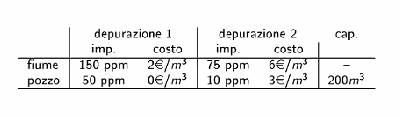
\includegraphics{tabella.png}
\end{figure}
Vediamo quindi che ogni giorno dalla falda acquifera non possiamo aspirare più di 200$m^3$ di acqua, mentre il fiume avoja a te prima de finillo. Abbiamo due depurazioni possibili, ma possiamo dire che la depurazione 1 per il pozzo non esiste, e considerarla come acqua estratta senza depurazione, poiché costa 0. Le variabili sono:
\begin{itemize}
    \item $x_{f,1}$ = q.tà di acqua di fiume depurata con la depurazione 1 $[m^3$/giorno]
    \item $x_{f,2}$ = q.tà di acqua di fiume depurata con la depurazione 2 $[m^3$/giorno]
    \item $x_{p,1}$ = q.tà di acqua di pozzo non depurata $[m^3$/giorno]
    \item $x_{p,2}$ = q.tà di acqua di pozzo depurata con la depurazione 2 [$m^3$/giorno]
\end{itemize}
I nostri vincoli allora sono;
\begin{equation*}
    x_{f,1} + x_{f,2} + x_{p,1} + x_{p,2} \geq 500
\end{equation*}
\begin{equation*}
    x_{p,1} + x_{p,2} \leq 200    
\end{equation*}
\begin{equation*}
    150x_{f,1} + 75x_{f,2} + 50x_{p,1} + 10x_{p,2} \leq 100(x_{f,1} + x_{f,2} + x_{p,1} + x_{p,2})
\end{equation*}
\begin{equation*}
    x_{f,1}, x_{f,2}, x_{p,1}, x_{p,2} \geq 0
\end{equation*}
Invece la funzione obiettivo è la funzione costo:
\begin{equation*}
min 8(x_{p,1}+x_{p,2}) + 2x_{f,1} + 6x_{f,2} + 3x_{P,2} 
\end{equation*}





\section{Autovalutazione 1:}


\paragraph{1. Classificare i problemi:} 
\begin{equation*}
min \hspace{0.3cm} -x_1 + 2x_2 + x_4 + 10x_5 + x_6 + x_7 
\end{equation*}
\begin{equation*}
    x_3 - x_4 \leq -1
\end{equation*}
\begin{equation*}
    x_5 -4x_6 \geq 0
\end{equation*}
\begin{equation*}
-x_1 + x_2 + x_7 = 10 
\end{equation*}
\begin{equation*}
x_1 \geq 0, x_2 \geq 0, x_4 \geq 0, x_5 \geq 0, x_7 \geq 0
\end{equation*}
Si tratta di un problema di ottimizzazione continua e vincolata. Precisamente, poiché il nostro insieme ammissibile è costituito da vincoli in forma di disuguaglianze (e uguaglianze), si tratta di un problema di Programmazione Matematica. Infine, poiché la funzione obiettivo e i vincoli sono lineari, questo problema si può classificare come un problema di Programmazione Matematica Lineare.

\vspace{0.2cm}

\begin{equation*}
min \hspace{0.3cm} -x_1^2 + x_4x_5 
\end{equation*}
\begin{equation*}
    x_3 - x_4^3 \leq -1
\end{equation*}
\begin{equation*}
    \frac{1}{x_5} - 4x_6 \geq 0
\end{equation*}
\begin{equation*}
    -x_1 + x_2 \geq 10 
\end{equation*}
\begin{equation*}
x_1 \geq 0, x_2 \geq 0
\end{equation*}
Si tratta di un problema di ottimizzazione continua e vincolata e, anche qui, di Programmazione Matematica. Stavolta però, dato che si presentano termini quadratici e cubici, prodotti tra variabili e dei reciproci, si tratta di Programmazione Matematica NonLineare.

\vspace{0.2cm}

\begin{equation*}
min \hspace{0.3cm} 10x_1 + x_2 + x_3 
\end{equation*}
\begin{equation*}
    x_1 - 4x_2 \geq 0
\end{equation*}
\begin{equation*}
    -x_1 + x_3 \leq 10
\end{equation*}
\begin{equation*}
    x_2 + x_3 = 1 
\end{equation*}
\begin{equation*}
    x_1 \in Z, x_2 \in Z, x_3 \in Z
\end{equation*}
Si tratta di un problema di ottimizzazione discreta, precisamente programmazione a numeri interi. Possiamo dire inoltre che il problema è di Programmazione Matematica Lineare.


\paragraph{Esercizio dell'industria:} 

\

\begin{figure}[h!]
    \centering
    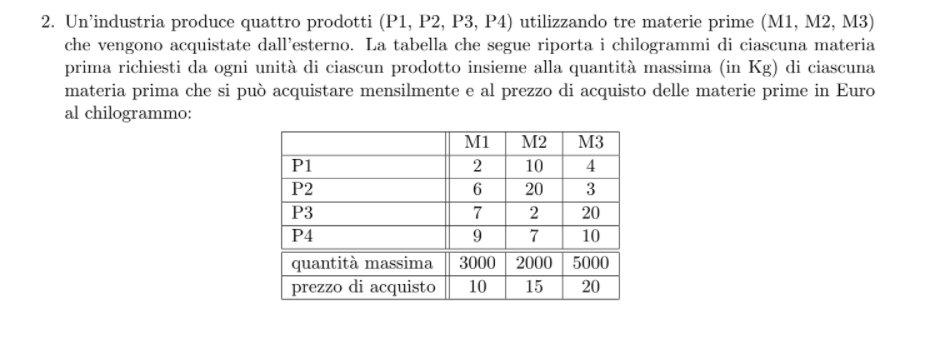
\includegraphics[scale=0.8]{autovalutazioneesercizio1.png}
\end{figure}

definendo
\begin{itemize}
    \item $x_1 \equiv$ q.tà di P1 prodotto [U/mese]
    \item $x_2 \equiv$ q.tà di P2 prodotto [U/mese]
    \item $x_3 \equiv$ q.tà di P3 prodotto [U/mese]
    \item $x_4 \equiv$ q.tà di P4 prodotto [U/mese]
    \item $y_1 \equiv$ q.tà di M1 acquistato [kg/mese] = $2x_1 + 6x_2 + 7x_3 + 9x_4$
    \item $y_2 \equiv$ q.tà di M2 acquistato [kg/mese] = $10x_1 + 20x_2 + 2x_3 + 7x_4$
    \item $y_3 \equiv$ q.tà di M3 acquistato [kg/mese] = $4x_1 + 3x_2 + 20x_3 + 10x_4$
\end{itemize}
la funzione \textit{ricavo} è:
\begin{equation*}
    R = 2x_1 + 2.5x_2 + 4x_3 + 3.5x_4 \hspace{1cm} \left[\frac{10^3 \text{\euro}}{mese}\right]
\end{equation*}
mentre la funzione costo è:
\begin{equation*}
    C = 10y_1 + 15y_2 + 20y_3 + 100\cdot10x_1 + 100\cdot12x_2 + 100\cdot20x_3 + 100\cdot18x_4 \left[\frac{\text{\euro}}{mese}\right]
\end{equation*}
Dove i primi tre addendi formano il costo relativo all'acquisto delle materie prime, mentre gli ultimi tre quello relativo alla lavorazione dei prodotti. Sostituendo a $y_i$ le espressioni in $x_i$, riscriviamo la funzione costo come:
\begin{equation*}
    C = 1.29x_1 + 1.65x_2 + 2.7x_3 + 2.295x_4 \hspace{1cm} [10^3 \text{\euro}]
\end{equation*}
La funzione obiettivo \textit{profitto netto} è quindi:
\begin{equation*}
    \text{max} \hspace{0.1cm} P = 2x_1 + 2.5x_2 + 4x_3 + 35x_4 - 1.29x_1 - 1.65x_2 - 2.7x_3 - 2.295x_4 = 
\end{equation*}
\begin{equation*}
    = 0.71 x_1 + 0.85 x_2 + 1.3 x_3 + 32.705 x_4 \left[\frac{10^3 \text{\euro}}{mese}\right]
\end{equation*}
Ma dobbiamo tenere in conto i seguenti vincoli:
\begin{equation*}
    x_i \geq 0, \hspace{0.2cm} \text{i $\in$ \{1,2,3,4\}}
\end{equation*}
\begin{equation*}
    y_1 = 2x_1 + 6x_2 + 7x_3 + 9x_4 \geq 0
\end{equation*}
\begin{equation*}
    y_2 = 10x_1 + 20x_2 + 2x_3 + 7x_4 \geq 0
\end{equation*}
\begin{equation*}
    y_3 = 4x_1 + 3x_2 + 20x_3 + 10x_4 \geq 0
\end{equation*}
\begin{equation*}
    y_1 = 2x_1 + 6x_2 + 7x_3 + 9x_4 \leq 3000
\end{equation*}
\begin{equation*}
    y_2 = 10x_1 + 20x_2 + 2x_3 + 7x_4 \leq 2000
\end{equation*}
\begin{equation*}
    y_3 = 4x_1 + 3x_2 + 20x_3 + 10x_4 \leq 5000
\end{equation*}
\begin{equation*}
    x_2 \leq (\frac{1}{4}x_1 + \frac{3}{10}x_2 + \frac{1}{2}x_3 + \frac{9}{20}x_4) 
\end{equation*}
Dove l'ultimo vincolo invece esprime matematicamente la condizione per cui le ore di lavorazione di P2 non possono superare il 30\% del totale delle ore di lavorazione di tutti i prodotti.



\paragraph{Questionario:} 

\subparagraph{1. Dire quali affermazioni sono corrette:}
\begin{itemize}
    \item[(a)] l’insieme ammissibile di un problema di Programmazione Matematica è descritto da un sistema di equazioni e disequazioni; \textcolor{green}{CORRETTA}
    \item[(b)] un problema di Programmazione Matematica può avere un numero infinito di vincoli; \textcolor{red}{NON CORRETTA}
    \item[(c)] un problema di Programmazione Matematica ammette sempre una soluzione ottima; \textcolor{red}{NON CORRETTA}: un problema ammette soluzione ottima se $\exists x^*\in S$ t.c. $f(x^*) \leq f(x), \forall x \in S$, ma prendendo come esempio un problema di Programmazione Matematica così definito:
    \begin{equation*}
        min f(x)
    \end{equation*}
    \begin{equation*}
        x \leq 1
    \end{equation*}
    \begin{equation*}
        x \geq 10
    \end{equation*}
    Essendo l'insieme ammissibile S $= \varnothing$, non può esistere $x^* \in S$ tale che valga quanto detto.
    \item[(d)] se in un punto $\bar{x}$ un vincolo di disuguaglianza è attivo, allora  $\bar{x}$ non soddisfa tale vincolo. \textcolor{red}{NON CORRETTA}
\end{itemize}


\subparagraph{2. Dire quali affermazioni sono corrette:}
\begin{itemize}
    \item[(a)] un problema di Programmazione Matematica con vincoli lineari si dice problema di Programmazione Lineare; \textcolor{red}{NON CORRETTA:} anche la funzione obiettivo deve essere lineare
    \item[(b)] l’insieme $S = \{x \in \mathbb{R}^3$ $| x_1 \cos2 + x_2\sin4 - x_3 \leq 10$, \hspace{0.05cm} $2x_1 - x_2 = 35\}$ può essere l'insieme ammissibile di un problema di Programmazione Lineare; \textcolor{green}{CORRETTA}
    \item[(c)] Il problema:
    \begin{equation*}
        \begin{cases}
            \text{min $2x_1 - x_2 + 5x_3$}\\
            \text{$x_1 + 2x_2 - 12x_3 \geq 4$}\\
            \text{$x_1 + 2 x_2 x_3 + 4x_3 \geq 5$}
        \end{cases}
    \end{equation*}
    è un problema di Programmazione Lineare; \textcolor{red}{NON CORRETTA}: $x_2 x_3$ rende l'ultima disequazione non lineare
    \item[(d)] l’insieme ammissibile di un problema di Programmazione Lineare può essere sempre espresso nella forma Ax $\geq$ b con A matrice m $\times$ n, $x \in \mathbb{R}^n$, b $\in \mathbb{R}^m$. \textcolor{green}{CORRETTA}
\end{itemize}




\section{Altro Risultato Importante:}
Abbiamo fatto un esercizio, prima dell'autovalutazione, che mostrava questo, ma in realtà si tratta di un vero e proprio risultato. Cioè se si ha un problema di PL:
\begin{equation*}
    min c^Tx
\end{equation*}
\begin{equation*}
    Ax \geq b
\end{equation*}
E valgono le seguenti condizioni:
\begin{itemize}
    \item P = \{x $\in \mathbb{R}^n$: $Ax \geq b$\} $\neq \varnothing$
    \item P non contiene rette
    \item Il problema non è illimitato inferiormente
\end{itemize}
Allora, prendendo un punto $\tilde{x}$ che non è un vertice, si può \textit{sempre costruire un vertice} $\bar{x} \in P$ tale che:
\begin{equation*}
    c^T\bar{x} \leq c^T\tilde{x}
\end{equation*}
Cioè un vertice che non peggiora (al più migliora) la funzione obiettivo rispetto a $\tilde{x}$. Tramite questo risultato riusciremo a dimostrare il \textit{Teorema Fondamentale della PL}.



\section{Teorema Fondamentale della PL:}
Supponiamo solo che P non contenga rette. Deve per forza accadere una e una sola delle seguenti cose:
\begin{itemize}
    \item P è vuoto (P = $\varnothing$)
    \item Il problema è illimitato inferiormente
    \item Il problema ammette soluzione ottima, magari ne ammette una sola, magari infinite, ma almeno una delle soluzioni ottime è un vertice di P
\end{itemize}
Il teorema si può applicare anche se P contiene rette, ma ci assicura soltanto che il problema ammette soluzioni ottime, senza garantirci che una di queste sia un vertice. Ad esempio prendiamo come poliedro di un problema il semipiano delle x positive:
\begin{equation*}
    x \geq 0
\end{equation*}
Vediamo che chiaramente non è nullo, e inoltre se il nostro problema è minimizzare x:
\begin{equation*}
    min \hspace{0.2cm} x
\end{equation*}
non è neanche un problema illimitato inferiormente (perché il minimo inferiore è x = 0). Quindi rimane solo l'ultimo caso, cioè quello che il problema ammetta soluzioni ottime, ed effettivamente è così: tutti i punti dell'asse delle ordinate sono soluzioni ottime. Ma vediamo che il poliedro $x \geq 0$ contiene interamente rette, ciò significa che non è detto che abbia vertici. Infatti non li ha. Per questo motivo possiamo usare il teorema fondamentale della PL e dire che, dato che P non è vuoto e il problema non è illimitato inferiormente, il problema deve ammettere soluzione ottima, ma il discorso è che non è vero che almeno una di queste soluzioni è un vertice. Quindi l'ipotesi di P che non contiene rette non è fondamentale per applicare il teorema fondamentale, ma è fondamentale se vogliamo applicarlo per trovare una soluzione che sia un VERTICE.

\paragraph{Dimostrazione:} Le tre affermazioni sono mutuamente esclusive, al massimo una di queste è vera. Questo non c'è bisogno di dimostrarlo, si vede. Dobbiamo però dimostrare che esattamente una, tra queste, è vera. Come facciamo? Fissiamo due false e proviamo che la terza è vera. Assumiamo che la prima e la seconda sono false, e facciamo vedere che la terza è vera.
\begin{itemize}
    \item se la prima affermazione è falsa vuol dire che P $\neq \varnothing$
    \item se la seconda affermazione è falsa vuol dire che il problema non è illimitato inferiormente
\end{itemize}
In più, da condizione del Teorema Fondamentale della PL, sappiamo che P non contiene rette. Quindi, abbiamo le ipotesi del risultato visto prima di questo:
\begin{itemize}
    \item P $\neq \varnothing$
    \item P non contiene rette
    \item P non è illimitato inferiormente
\end{itemize}
Inoltre, abbiamo dimostrato come secondo risultato importante che se P è non nullo e non contiene interamente rette allora P ammette un numero FINITO e maggiore di 0 di vertici. Quindi possiamo dire, proprio per il risultato visto prima che è possibile costruire un vertice che non peggiori (al più migliori) la funzione obiettivo partendo da un punto del poliedro che non è un vertice. Bene, adesso ci si presentano 2 casi:
\begin{itemize}
    \item P = \{$\bar{x}$\}. Cioè il poliedro è un singleton con un solo elemento. Chiaramente per i risultati sopra $\bar{x}$ deve essere un vertice e l'unica soluzione ottima del problema di PL, quindi abbiamo dimostrato ciò che ci serviva
    \item P è costituito da infinite soluzioni
\end{itemize}
\underline{Non può infatti accadere che P abbia un numero finito di punti}\footnote{Questo vale in generale!}, poiché essendo un insieme convesso, ogni singolo punto del segmento che congiunge due punti di P deve appartenere a P, e un segmento ha infiniti punti. Il terzo caso, che si presenta in generale ma che non si può presentare in questo caso per le ipotesi, è che il poliedro sia vuoto, altro un poliedro non può essere. Prendiamo quindi il nostro secondo caso. Per quanto abbiamo detto sappiamo che P ammette $r > 0$ vertici, che chiamiamo $v_i$ con i = 1, 2, ..., r. Su ciascuno di questi vertici posso calcolare la funzione obiettivo, trovando r numeri. Di questi posso prendere il minimo (o uno dei minimi, se ce ne sono più di uno):
\begin{equation*}
    min\{c^T_1, ..., c^Tv_r\} = c^Tv_h \hspace{1cm} h \in \{1,...,r\}
\end{equation*}
Prendiamo adesso un punto qualsiasi x del nostro poliedro $x \in P$. Sappiamo che, per quanto detto, possiamo costruire, a partire da questo punto qualsiasi, un vertice, uno degli r qua sopra, chiamiamolo:
\begin{equation*}
    v_i: \hspace{0.5cm} c^Tv_i \leq c^Tx
\end{equation*}
Ora, dato che $v_h$ è il migliore tra i vertici (a parimerito con altri minimi eventualmente), si ha che:
\begin{equation*}
    c^Tv_h \leq c^Tv_i \leq c^Tx
\end{equation*}
Dove x è il mio punto qualsiasi. Questo vale $\forall x \in P$, quindi $v_h$ è un vertice e una soluzione ottima del problema, dimostrando che c'è per forza una e una sola delle 3 possibilità che è vera. $\square$



\subsection{Vediamo qualche caso particolare:} Per esempio, se consideriamo un PL in cui sappiamo che l'insieme delle soluzioni ammissibili P è un \textit{politopo}. \textit{Come diventa il teorema fondamentale della PL quando P è un politopo}? Se P è un politopo non dobbiamo ipotizzare che P non contiene rette, perché P è un politopo, quindi limitato, quindi ovvio che non contiene rette. Il risultato torna ai tre possibili risultati del teorema fondamentale.

\vspace{1cm}

\noindent Altra soluzione: supponiamo che il seguente problema di PL:
\begin{equation*}
    min \hspace{0.3cm} c^Tx
\end{equation*}
\begin{equation*}
    Ax \geq b
\end{equation*}
(\textcolor{red}{lui ha scritto 0 ma ha detto b secondo me è giusto b e si è sbagliato a scrivere}) Ammetta due soluzioni ottime, $\tilde{x}$ e $\bar{x}$ diverse tra loro. Ora, siccome sono entrambe ottime deve valere:
\begin{equation*}
    c^T\bar{x} = c^T\tilde{x}
\end{equation*}
Ora consideriamo il segmento [$\bar{x}$, $\tilde{x}$] che ha come estremi appunto queste due soluzioni ottime. Possiamo scrivere così questo segmento:
\begin{equation*}
    x(\lambda) = \lambda\bar{x} + (1 - \lambda)\tilde{x} \hspace{1cm} \lambda \in [0,1]
\end{equation*}
Quindi è vero che:
\begin{equation*}
    c^Tx(\lambda) = \lambda c^T\bar{x} + (1-\lambda)c^T\tilde{x} = \lambda c^T\bar{x} + (1-\lambda)c^T\bar{x} = c^T\bar{x} = c^T\tilde{x}
\end{equation*}
Quindi questo significa che se ho due soluzioni ottime ne ho in realtà infinite, almeno tutte quelle sul segmento $x(\lambda)$, proprio perché $c^Tx(\lambda)$ ha lo stesso valore delle due soluzioni ottime.

\vspace{1cm}

\noindent Altro caso, abbiamo un problema di PL con almeno una soluzione ottima $x^*$, se il problema ammette anche altre soluzioni ottime oltre questa, deve valere:
\begin{equation*}
    c^Tx = c^Tx^*
\end{equation*}
Queste soluzioni ottime devono essere ammissibili, quindi devono soddisfare questo:
\begin{equation*}
    Ax \geq b
\end{equation*} 
Ora, l'insieme:
\begin{equation*}
    P^* = \{x \in \mathbb{R}^n: Ax \geq b, c^Tx = c^Tx^*\}
\end{equation*}
Deviamo che è un insieme definito dall'intersezione di un numero finito di semispazi chiusi (quelli rappresentati dal sistema Ax$\geq$b) e da un iperpiano ($c^Tx = c^Tx^*$), quindi anche $P^*$ è un poliedro. Ciò che vuol dire: che \textit{in un problema di PL che ammette soluzione ottima, l'insieme delle soluzioni ottime è un Poliedro}. Quindi sia zona ammissibile che insieme soluzioni ottime sono poliedri. Poiché un poliedro può solo essere vuoto, ammette un solo punto o ammettere infiniti punti, questo vuol dire che \textit{l'insieme delle soluzioni ottime di un problema di PL può essere vuoto (quindi non ci sono soluzioni ottime), ammettere un singolo punto (c'è una singola soluzione ottima), ammettere infiniti punti (ci sono infinite soluzioni ottime)}.

\vspace{1cm}

\noindent Altra cosa: se P è un politopo non vuoto di un problema di PL, certamente esiste almeno una soluzione ottimale e almeno una soluzione ottimale che è un vertice. Per verificarlo usiamo il T.F. della PL: se P è un politopo non vuoto non può essere vuoto; se P è un politopo il problema di PL non può essere illimitato inferiormente, poiché P è limitato. Quindi rimane l'ultima possibilità del T.F. della PL: P ammette almeno una soluzione ottima, e almeno una soluzione ottima che è un vertice.

\newpage

\section{Facciamo un esercizio, Problema inferiormente illimitato:}

\begin{equation*}
    min \hspace{0.5cm} -5x_1 -7x_2
\end{equation*}
\begin{equation*}
    c. v. \hspace{0.5cm} -3x_1 + 2x_2 \leq 30
\end{equation*}
\begin{equation*}
    -2x_1 + x_2 \leq 12
\end{equation*}
\begin{equation*}
    x_1 \geq 0, x_2 \geq 0
\end{equation*}
Vediamo già che l'origine è un punto ammissibile, che soddisfa tutti i vincoli. Ciò significa che il poliedro non è vuoto. Inoltre vediamo che, essendo quest'ultimo interamente contenuto nel primo quadrante, sicuro non c'è nessuna retta che è interamente contenuta dentro il poliedro. Quindi poliedro non nullo e non contenente interamente rette significa, per il secondo risultato importante che abbiamo trovato, che il poliedro ammette almeno un vertice. Graficando infatti troviamo tre vertici:
\begin{figure}[h!]
    \centering
    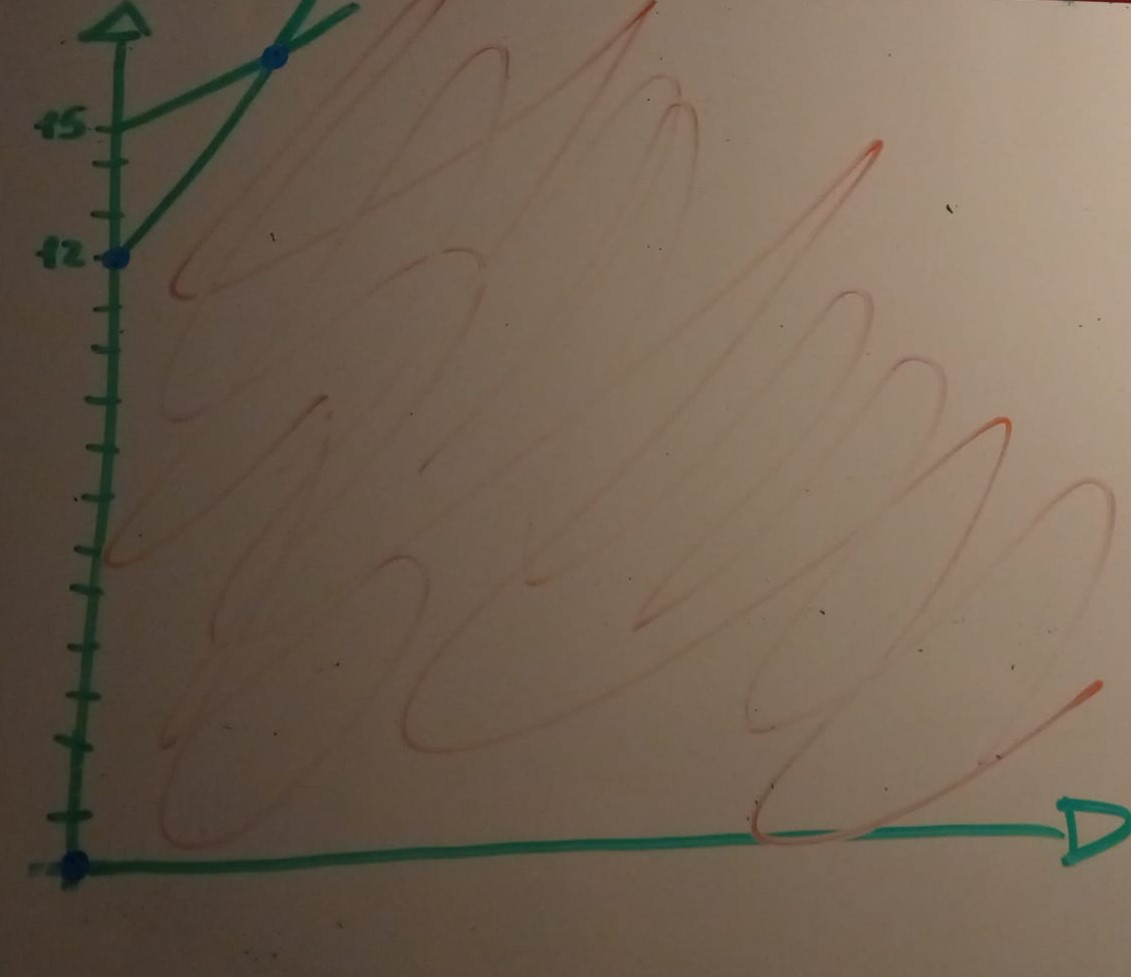
\includegraphics[scale=0.3]{WhatsAppImage2021-10-17at23.52.07.jpeg}
\end{figure}
Ora passiamo alla funzione obiettivo
\begin{equation*}
    -5x_1 -7x_2 = k
\end{equation*}
Vediamo che il vettore dei coefficienti è:
\begin{equation*}
    c = \begin{pmatrix}
        -5 & -7
    \end{pmatrix}
\end{equation*}
Che indica un vettore nel III quadrante. Le rette del fascio $-5x_1 -7x_2 = k$ sono ortogonali a questo vettore. Inoltre \textbf{questo vettore indica dove cresce la funzione obiettivo} \textbf{IMPORTANTE!!!} Quindi la funzione cresce se si abbassa, siccome noi vogliamo minimizzarla dobbiamo spostarci nella parte opposta al vettore, quindi verso l'alto.
\begin{figure}[h!]
    \centering
    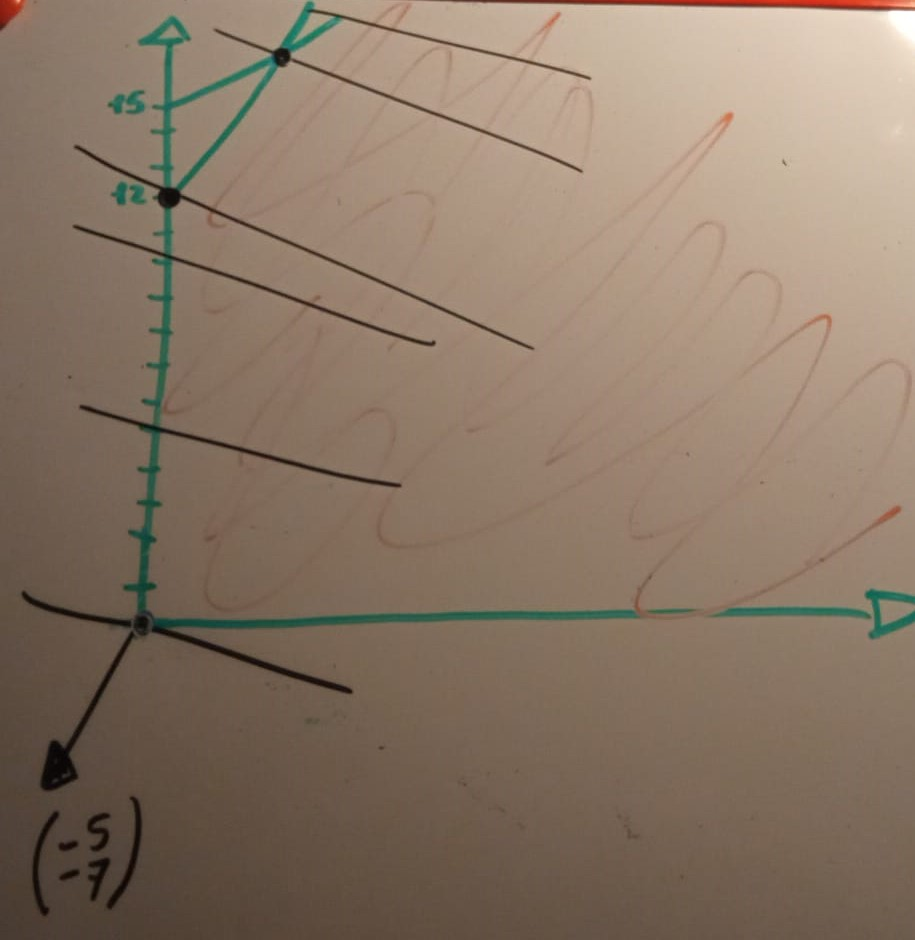
\includegraphics[scale=0.3]{WhatsAppImage2021-10-18at00.03.51.jpeg}
\end{figure}
Vediamo, calcolando la funzione obiettivo in ognuno dei tre vertici, che nessuno dei tre è effettivamente soluzione ottima, poiché andando ancora di più verso l'alto troviamo valori più bassi di quelli dei vertici. Quindi, poiché P non è vuoto, e il problema non ammette soluzione ottima, per il T.F. della PL il problema è illimitato inferiormente.


\newpage

\section{Quando c'è più di una soluzione ottima:}
\begin{equation*}
    min x_1 - 2x_2
\end{equation*}
\begin{equation*}
    x_1 - 2x_2 \geq 4
\end{equation*}
\begin{equation*}
    x_1 + x_2 \leq 8
\end{equation*}
\begin{equation*}
    x_1 \geq 0, x_2 \geq 0
\end{equation*}
Vediamo che il politopo che fa da zona ammissibile è il seguente
\begin{figure}[h!]
    \centering
    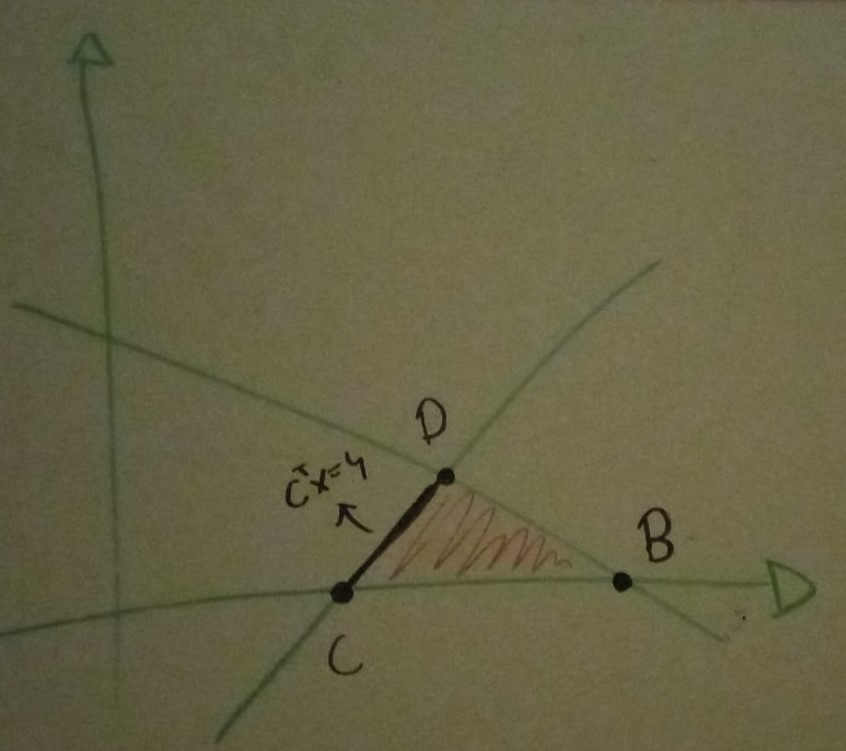
\includegraphics[scale=0.3]{bho.jpeg}
\end{figure}
Nei vertici abbiamo:
\begin{equation*}
    c^TD = 4
\end{equation*}
\begin{equation*}
    c^TC = 4
\end{equation*}
\begin{equation*}
    c^TB = 8
\end{equation*}
\textbf{ATTENZIONE! Vediamo quindi che sono due i vertici in cui la soluzione è ottima, ma abbiamo detto che non possono esserci 2 soluzioni ottime!} O un'unica soluzione ottima o infinite! Infatti la soluzione è \textbf{Il segmento che congiunge C e D}. Quindi quando non c'è un'unica soluzione considera il segmento tra le due soluzioni come insieme delle soluzioni.


\newpage

\section{Caso particolare, problema inammissibile:}
\begin{equation*}
    min 3x_1 + x_2
\end{equation*}
\begin{equation*}
    x_1 - x_2 \geq 1
\end{equation*}
\begin{equation*}
    3x_1 + 2x_2 \leq 12
\end{equation*}
\begin{equation*}
    2x_1 + 3x_2 \leq 3
\end{equation*}
\begin{equation*}
    -2x_1 + 3x_2 \geq 9
\end{equation*}
\begin{equation*}
    x_1 \geq 0, x_2 \geq 0
\end{equation*}
Siamo sempre nel quadrante positivo.
\begin{figure}[h!]
    \centering
    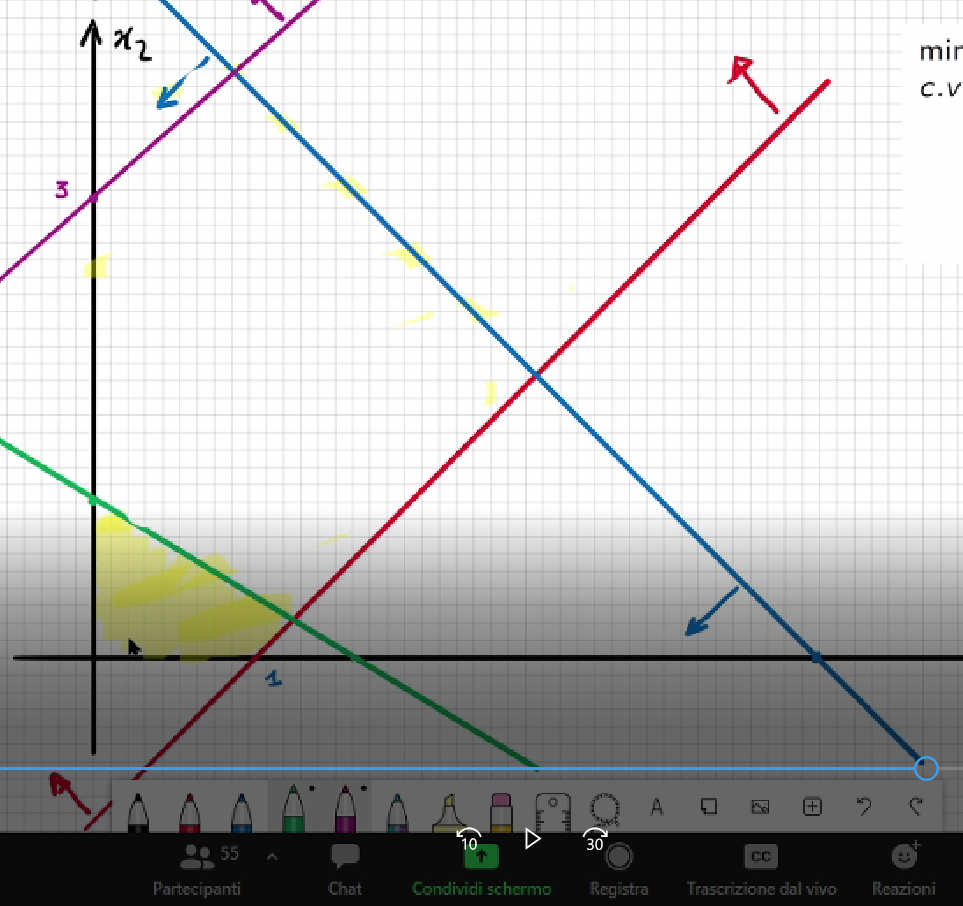
\includegraphics[scale=0.5]{okok.png}
\end{figure}
Vediamo che, secondo tutte le disuguaglianze, i punti del poliedro dovrebbero essere nell'intersezione tra la zona gialla e sopra la retta viola. Ma quell'intersezione è nulla. \textit{Quindi la soluzione del problema c'è ed è: il problema non è ammissibile, perché P} $= \varnothing$.






\section{Esercizio:} 
Vediamo questo esercizio:
\begin{figure}[h!]
    \centering
    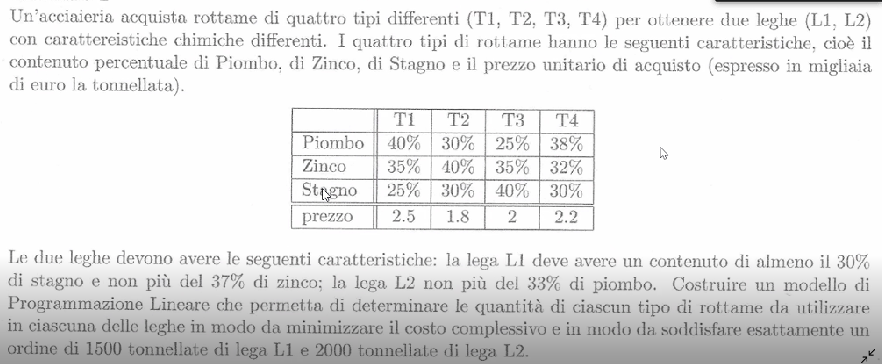
\includegraphics[scale=0.5]{Esercizietto.png}
\end{figure}

\subparagraph{Risposta:}
abbiamo le seguenti variabili:
\begin{equation*}
    x_{i,j} \hspace{0.5cm} \text{i-esimo rottame usato nella j-esima lega} [tonnellate]
\end{equation*}
Abbiamo la funzione obiettivo:
\begin{equation*}
    min \hspace{0.2cm} 2.5(x_{1,1} + x_{1,2}) + 1.8(x_{2,1} + x_{2,2}) + 2(x_{3,1} + x_{3,2}) + 2.2(x_{4,1} + x_{4,2}) [migliaia di \euro] 
\end{equation*}
Ora vediamo i vincoli:
\begin{equation*}
    x_{i,j} \geq 0
\end{equation*}
\begin{equation*}
    25\%x_{1,1} + 30\%x_{2,1} + 40\%x_{3,1} + 30\%x_{4,1} \geq 30\%(x_{1,1} + x_{2,1} + x_{3,1} + x_{4,1}) 
\end{equation*}
\begin{equation*}
    35\%x_{1,1} + 40\%x_{2,1} + 35\%x_{3,1} + 32\%x_{4,1} \leq 37\%(x_{1,1} + x_{2,1} + x_{3,1} + x_{4,1}) 
\end{equation*}
\begin{equation*}
    40\%x_{1,2} + 30\%x_{2,2} + 25\%x_{3,2} + 38\%x_{4,2} \leq 33\%(x_{1,2} + x_{2,2} + x_{3,2} + x_{4,2}) 
\end{equation*}
\begin{equation*}
    x_{1,1} + x_{2,1} + x_{3,1} + x_{4,1} = 1500 [tonnellate]
\end{equation*}
\begin{equation*}
    x_{1,2} + x_{2,2} + x_{3,2} + x_{4,2} = 2000 [tonnellate]
\end{equation*}





\section{Equivalenza di due Problemi :} 
La forma generale di PL: 
\begin{equation*}
    Ax \geq b    
\end{equation*}
Si presta male quando dobbiamo computazionalmente risolvere il problema e scoprire se:
\begin{itemize}
    \item Il poliedro è vuoto (problema inammissibile)
    \item Il problema è illimitato inferiormente
    \item Il problema ammette soluzioni ottime e almeno una di queste è un vertice
\end{itemize}
Una forma più comoda per questo e generale allo stesso livello è quella standard. Possiamo usare questa forma perché è \textbf{Equivalente} a quella generale. Ma che vuol dire che è equivalente? 

\subsection{Definizione di equivalenza tra problemi:}

Se il problema (P) di ottimizzazione è:
\begin{equation*}
    min f(x)
\end{equation*}
\begin{equation*}
    c.v. x \in S \subseteq \mathbb{R}^n
\end{equation*}
Mentre il problema (Q) di ottimizzazione è:
\begin{equation*}
    min g(w)
\end{equation*}
\begin{equation*}
    c.v. w \in D \subseteq \mathbb{R}^m
\end{equation*}
I problemi (P) e (Q) sono equivalenti se e solo se:
\begin{itemize}
    \item è possibile stabilire una corrispondenza tra le soluzioni dei due problemi. Cioè determinata una soluzione di (P) io posso determinare una soluzione di (Q)
    \item (P) ammette soluzione ottima $\Longleftrightarrow$ (Q) ammette soluzione ottima
\end{itemize}
Ok, ma sta definizione operativamente non la posso usare per trovare se due problemi sono equivalenti. Usiamo un criterio di equivalenza che invece viene usato operativamente:

\paragraph{Criterio di Equivalenza:}
Dati i due problemi di ottimizzazione (P) e (Q):
\begin{equation*}
    min f(x)
\end{equation*}
\begin{equation*}
    c.v. x \in S \subseteq \mathbb{R}^n
\end{equation*}

\begin{equation*}
    min g(w)
\end{equation*}
\begin{equation*}
    c.v. w \in D \subseteq \mathbb{R}^m
\end{equation*}
Se è vero che
\begin{itemize}
    \item[1.] $\forall x \in S$ $\exists w \in D$ t.c. $g(w) \leq f(x)$
    \item[2.] $\forall w \in D$ $\exists x \in S$ t.c. $f(x) \leq g(w)$
\end{itemize}
allora f ha un minimo globale su S $\Longleftrightarrow$ g ha un minimo globale su D

\subparagraph{Dimostrazione del Criterio di Equivalenza:} 

Partiamo dall'ipotesi due: supponiamo che il problema (Q) ammetta soluzione ottima globale, chiamiamola $w^*$. Per la seconda ipotesi si ha che dato $w = w^* \in  D$:
\begin{equation*}
    \exists x^* \in S \hspace{0.1cm} \text{t.c.} \hspace{0.1cm} f(x^*) \leq g(w^*)
\end{equation*}
Dimostriamo che questo $x^*$ è un minimo globale. In questo modo avremo dimostrato che:
\begin{equation*}
    \text{g ha un minimo globale $w^*$ su D} \implies \text{f ha un minimo globale $x^*$ su S}
\end{equation*}
Quindi solo l'implicazione di destra. Come dimostriamo che $x^*$ sia soluzione globale? Lo facciamo per assurdo. Quindi supponiamo che $x^*$ non sia soluzione globale di (P) su S. Quindi, se $x^*$ non è soluzione vale allora $\exists \bar{x} \in S$ t.c.:
\begin{equation*}
    f(\bar{x}) < f(x^*)
\end{equation*}
Dato che per convenzione poniamo come soluzione ottima il minimo, perché per convenzione il nostro problema è un problema di minimo. Ok, quindi abbiamo un punto $\bar{x} \in S$. Per questo sicuramente vale la prima ipotesi, cioè dato $x = \bar{x} \in  S$:
\begin{equation*}
    \exists \bar{w} \in D \hspace{0.1cm} \text{t.c.} \hspace{0.1cm} g(\bar{w}) \leq f(\bar{x})
\end{equation*}
Ok, ora ricordiamoci che abbiamo posto $w^*$ come soluzione ottima su D, quindi deve valere:
\begin{equation*}
    g(w^*) \leq g(\bar{w})
\end{equation*}
E per quanto appena trovato su $\bar{w}$ e $\bar{x}$:
\begin{equation*}
    g(w^*) \leq g(\bar{w}) \leq f(\bar{x}) < f(x^*)
\end{equation*}
Ma per il fatto che abbiamo supposto che il problema (Q) ammettesse il punto $w^*$ t.c. $f(x^*) \leq g(w^*)$ si ha che:
\begin{equation*}
    g(w^*) < f(x^*) \leq g(w^*) \implies g(w^*) < g(w^*)
\end{equation*}
Che è assurdo! Ora dovremmo far vedere l'altra implicazione, cioè che:
\begin{equation*}
    \text{g ha un minimo globale $w^*$ su D} \impliedby \text{f ha un minimo globale $x^*$ su S} 
\end{equation*}
Ma i passaggi sono gli stessi identici, serve solo mettere in ordine inverso i termini. $\square$



\subsection{Facciamo un esempio di problemi equivalenti, un esempio molto particolare:} 
Abbiamo il problema (P):
\begin{equation*}
    min \hspace{0.1cm} c^Tx
\end{equation*}
\begin{equation*}
    c.v. \hspace{0.1cm} Ax \geq b
\end{equation*}
E il problema (Q):
\begin{equation*}
    min \hspace{0.1cm} c^T(y-z)
\end{equation*}
\begin{equation*}
    c.v. \hspace{0.1cm} A(y-z) - u = b
\end{equation*}
\begin{equation*}
    y,z \geq 0_n, u \geq 0_m
\end{equation*}
Facciamo vedere che i due problemi sono equivalenti. Vediamo innanzitutto che i due problemi \textbf{sono proprio in due spazi diversi}, perché il primo ha
\begin{equation*}
    A \in \mathbb{R}^{m \times n} \hspace{1cm} b \in \mathbb{R}^m \hspace{1cm} x \in \mathbb{R}^n
\end{equation*}
Cioè ha n variabili $x_i$ (uguali al numero di colonne di A), mentre il secondo ha:
\begin{equation*}
    A \in \mathbb{R}^{m \times n} \hspace{1cm} b \in \mathbb{R}^m \hspace{1cm} y,z \in \mathbb{R}^n \hspace{1cm} u \in \mathbb{R}^m
\end{equation*}
Cioè ha 2n + m variabili $y_i$, $z_i$ e $u_i$. Ok, comunque, andiamo a verificare le due ipotesi del criterio di equivalenza:
\begin{enumerate}
    \item $\forall x \in S$ $\exists w \in D$ (poi dopo agiremo sulle funzioni obiettivo, per ora concentriamoci sul costruire w t.c. sia ammissibile). Che nel nostro caso significa: prendiamo una $x \in S$, cioè che sia ammissibile per il seguente sistema:
    \begin{equation*}
        Ax \geq b
    \end{equation*}
    Allora data questa x generica dobbiamo essere in grado di trovare una w, che nel nostro caso sono tre variabili: y,z e u che appartengano a D, cioè che siano ammissibili per il seguente sistema:
    \begin{equation*}
        A(y-z) - u = b
    \end{equation*}
    E siano inoltre tutte non negative. Quindi a partire da x \textbf{COSTRUISCO} y,z e u come mi sono comode per soddisfare i vincoli di D. Ok come facciamo, innanzitutto definisco:
    \begin{equation*}
        u = Ax - b
    \end{equation*}
    Perché mi fa comodo. Vediamo infatti che, dato che $Ax \geq b$, cioè $Ax - b \geq b$, già u soddisfa un vincolo, cioè:
    \begin{equation*}
        u \geq 0_m
    \end{equation*}
    Ora tocca a y e z. Definisco, sempre perché mi fa comodo, le componenti di $x$, cioè le $x_i$, in questa maniera:
    \begin{itemize}
        \item Se $x_i \geq 0$ allora definisco $y_i = x_i$ e $z_i = 0$
        \item Se $x_i \leq 0$ allora definisco $y_i = 0$ e $z_i = -x_i$
    \end{itemize}
    Questo io lo faccio per ogni componente i di x. Già da questa decisione che abbiamo fatto vediamo che, per come li abbiamo definiti, $y_i$ e $z_i$ non possono essere negativi. Quindi abbiamo fatto soddisfare tutti e tre i vincoli di non negatività, ci manca solo $A(y-z)-u = b$. Vediamo che, sempre per come li abbiamo definiti, per ogni componente vale:
    \begin{equation*}
        x_i = y_i - z_i
    \end{equation*}
    E proprio perché vale per ogni componente si ha:
    \begin{equation*}
        x = y - z
    \end{equation*}
    E daje abbiamo costruito y e z, avendo già verificato i vincoli di non negatività, adesso occupiamoci dell'ultimo:
    \begin{equation*}
        A(y - z) - u = b \Longleftrightarrow Ax - Ax + b = b \implies \text{b = b che è VERA}
    \end{equation*}
    Avendo utilizzato due relazioni: la prima è quella che abbiamo appena trovato, cioè x = y - z, mentre la seconda è u = Ax - b, fatta all'inizio della dimostrazione. Quindi, a partire da una x ammissibie per il problema (P) abbiamo definito e costruito u, y e z in modo che soddisfino ogni vincolo del loro problema di (Q). Ok, avendo costruito delle variabili che sono ammissibili per (Q) adesso ci rimane solo da verificare la relazione sulle funzioni obiettivo, cioè la seconda parte della definizione:
    \begin{equation*}
        \forall x \in S \exists w \in D t.c. g(w) \leq f(x)
    \end{equation*}
    Che nel nostro caso diventa:
    \begin{equation*}
        c^T(y - z) \leq c^Tx \implies c^Tx \leq c^Tx \implies \text{VERA}
    \end{equation*}
    Avendo utilizzato il fatto che x = y - z. Ok ipotesi 1 verificata, occupiamoci della 2.
    
    
    \item  In questo caso facciamo l'inverso rispetto a prima. Cioè abbiamo y,z e u che soddisfano il problema (Q) e dobbiamo costruire x che soddisfi il problema (P), poi verificare la disuguaglianza sulle funzioni obiettivo. Ok cominciamo: abbiamo y,z e u t.c.:
    \begin{equation*}
        A(y - z) - u = b
    \end{equation*}
    \begin{equation*}
        y,z \geq 0_n \hspace{1cm} u \geq 0_m
    \end{equation*}
    Costruiamo ora x, in questa maniera:
    \begin{equation*}
        x = y - z
    \end{equation*}
    Ma x deve essere ammissibile per il suo problema:
    \begin{equation*}
        Ax \geq b
    \end{equation*}
    Vediamo che possiamo, per come abbiamo appena definito x, scrivere:
    \begin{equation*}
        Ax = A(y - z) = b + u \geq b
    \end{equation*}
    Dove l'ultima uguaglianza discende dal problema (Q), dove si ha come vincolo $A(y - z) - u = b$. Bene, quindi abbiamo:
    \begin{equation*}
        b + u \geq b 
    \end{equation*}
    E poiché $u \geq 0$ la disuguaglianza è verificata, quindi x è ammissibile per il problema (P). Ok, adesso dobbiamo vedere le funzioni obiettivo.
    \begin{equation*}
        c^Tx \leq c^T(y-z) \implies \text{VERO}
    \end{equation*}
    Per le stesse motivazioni del punto 1, dato che questa disuguaglianza è verificata in realtà all'uguaglianza. Abbiamo quindi verificato che \textbf{i due problemi (P) e (Q) sono equivalenti}.
\end{enumerate}
Il vantaggio è che, è vero che abbiamo due problemi equivalenti, ma uno dei due è più comodo computazionalmente. Difatti siamo passati dalla forma:
\begin{equation*}
    min \hspace{0.1cm} c^Tx
\end{equation*}
\begin{equation*}
    c.v. \hspace{0.1cm} Ax \geq b
\end{equation*}
Che è la cosiddetta \textit{forma generale}, alla forma:
\begin{equation*}
    min \hspace{0.1cm} c^T(y-z)
\end{equation*}
\begin{equation*}
    c.v. \hspace{0.1cm} A(y-z) - u = b
\end{equation*}
\begin{equation*}
    y,z \geq 0_n, u \geq 0_m
\end{equation*}
Che viene chiamata \textit{forma standard}, una particolare forma generale, che è molto comoda. Riscriviamo ora la forma standard compattamente. Definiamo:
\begin{equation*}
    \tilde{x} = \begin{pmatrix}
        y\\
        z\\
        u
    \end{pmatrix} \in \mathbb{R}^{2n + m} \hspace{1cm} \tilde{c}^T = \begin{pmatrix}
        c^T & -c^T & 0_m^T
    \end{pmatrix} \in \mathbb{R}^{2n+m}
\end{equation*}
Dove vediamo che il vettore trasposto $\tilde{c}^T$ presenta $c^T$, che ha n componenti, $-c^T$ che sono altre n componenti, e $0_m^T$ che sono m componenti. Quindi è una riga di 2n + m componenti. Infine definiamo:
\begin{equation*}
    \tilde{A} = \begin{pmatrix}
        A & -A & -I_m
        \end{pmatrix} \in \mathbb{R}^{m \times 2n + m}
\end{equation*}
Con queste definizioni, posso riscrivere il problema in forma standard in questa forma:
\begin{equation*}
    min \hspace{0.1cm} \tilde{c}^T\tilde{x}
\end{equation*}
\begin{equation*}
    \tilde{A}\tilde{x} = b
\end{equation*}
\begin{equation*}
    \tilde{x} \geq 0_{2n + m}
\end{equation*}
\textcolor{red}{SULLE SLIDE QUELLO CHE C'E' SCRITTO SU tilde x, tilde c ecc. E' TUTTO SBAGLIATO}. Quindi abbiamo verificato che \textbf{qualunque problema di PL è equivalente ad un problema di PL con soli vincoli di uguaglianza e tutte le variabili vincolate ad essere non negative}.




\section{Facciamo un esempio:} partiamo da una forma generale e trasformiamola in forma standard.
\begin{equation*}
    min \hspace{0.1cm} x_1 + x_2 - 3x_3 + 2x_4
\end{equation*}
\begin{equation*}
    x_1 - 2x_2 \geq 8
\end{equation*}
\begin{equation*}
    x_2 + x_3 \leq 6
\end{equation*}
\begin{equation*}
    x_4 \geq 0
\end{equation*}
Ok è in forma normale, innanzitutto riscriviamola in forma compatta però:
\begin{equation*}
    min \hspace{0.1cm} \begin{pmatrix}
        1 & 1 & -3 & 2
    \end{pmatrix}x
\end{equation*}
\begin{equation*}
    \begin{pmatrix}
        1 & -2 & 0 & 0\\
        0 & -1 & -1 & 0\\
        0 & 0 & 0 & 1
    \end{pmatrix}x \geq \begin{pmatrix}
        8\\
        -6\\
        0
    \end{pmatrix}
\end{equation*}
Adesso dobbiamo trasformarla in forma standard equivalente, sempre usando x = y - z e aggiungendo il vettore u:
\begin{equation*}
    min \hspace{0.1cm} \begin{pmatrix}
        1 & 1 & -3 & 2
    \end{pmatrix}(y-z) 
\end{equation*}
\begin{equation*}
    \begin{pmatrix}
        1 & -2 & 0 & 0\\
        0 & -1 & -1 & 0\\
        0 & 0 & 0 & 1
    \end{pmatrix}(y-z) - \begin{pmatrix}
        u_1\\
        u_2\\
        u_3\\
    \end{pmatrix} = \begin{pmatrix}
        8\\\
        -6\\
        0
    \end{pmatrix}
\end{equation*}
\begin{equation*}
    y_i, z_i, u_j \geq 0 \hspace{1cm} \forall i = 1,2,3,4 \hspace{0.2cm} \forall j = 1,2,3
\end{equation*}
E questa è la forma standard compatta. Eventualmente possiamo svolgere i prodotti e scriverla così:
\begin{equation*}
    min \hspace{0.1cm} y_1 - z_1 + y_2 - z_2 -3y_z + 3z_3 + 2y_4 - 2z_4  
\end{equation*}
\begin{equation*}
    y_1 - z_1 - 2y_2 + 2z_2 - u_1 = 8
\end{equation*}
\begin{equation*}
    - y_2 + z_2 -y_3 + z_3 + u_2 = -6
\end{equation*}
\begin{equation*}
    y_4 - z_4 + u_3 = 0
\end{equation*}
\begin{equation*}
    y_i, z_i, u_j \geq 0 \hspace{1cm} \forall i = 1,2,3,4 \hspace{0.2cm} \forall j = 1,2,3
\end{equation*}
Questa è la strada che il professore ha chiamato "scarpone", perché è quella in cui fai tutti i calcoli e la meno rapida. Si può comunque, evitare di fare tutti tutti i calcoli adottando \textit{alcune strategie che velocizzano la cosa} che ora vedremo. Prendiamo questo esempio:
\begin{equation*}
    min \hspace{0.1cm} x_1 - x_2 + x_3 + 2x_4
\end{equation*}
\begin{equation*}
    x_1 + x_2 + x_3 + x_4 = 7
\end{equation*}
\begin{equation*}
    x_2 + 3x_3 \leq 5
\end{equation*}
\begin{equation*}
    x_2 \leq 0
\end{equation*}
\begin{equation*}
    x_4 \geq 0
\end{equation*}
\textbf{Prima Strategia,} vediamo che abbiamo:
\begin{equation*}
    x_4 \geq 0
\end{equation*}
e dato che in forma standard noi dobbiamo avere tutte le variabili che denotano quantità non negative, sfrutto questa disequazione e la userò direttamente nella mia forma standard, senza adottare la sostituzione $x_4 = y_4 - z_4$. Si dice che $x_4$ \textit{non mi costa}, mentre le variabili che dovrò sostituire per raggiungere la forma standard \textit{mi costano}. La stessa cosa si potrebbe fare con:
\begin{equation*}
    x_2 \leq 0 \implies - x_2 \geq 0
\end{equation*}
Ma ignoriamolo. Bene, \textbf{Seconda Strategia,} vediamo che c'è già un vincolo di uguaglianza nella nostra forma genereale:
\begin{equation*}
    x_1 + x_2 + x_3 + x_4 = 7
\end{equation*}
Questo vuol dire che per questo vincolo non dovremo dalla forma $ax - u \geq b$ alla forma $a(y_i-z-i)-u_i = b$, perché già siamo nella forma con l'uguaglianza, semplicemente u = 0. Ok possiamo riscrivere il nostro problema in forma standard ora:
\begin{equation*}
    min \hspace{0.1cm} y_1 - z_1 - y_2 + z_2 + y_3 - z_3 + 2x_4  
\end{equation*}
\begin{equation*}
    y_1 - z_1 + y_2 - z_2 + y_3 - z_3 + x_4 = 7
\end{equation*}
\begin{equation*}
    y_2 - z_2 + 3y_3 - 3z_3 + u_1 = 5
\end{equation*}
\begin{equation*}
    y_2 - z_2 + u_2 = 0
\end{equation*}
\begin{equation*}
    x_4 \geq 0 \hspace{0.5cm} y_i, z_i, u_j \geq 0 \hspace{1cm} \forall i = 1,2,3,4 \hspace{0.2cm} \forall j = 1,2,3
\end{equation*}
Ora attenzione al terzo vincolo: 
\begin{equation*}
    y_2 - z_2 + u_2 = 0 \implies u_2 = -(y_2 - z_2) = -x_2
\end{equation*}
possiamo adottare una \textbf{Terza Strategia} e sostituire $\pm u_2$ ad ogni $y_z - z_2$ che incontriamo. Il fatto che io usi $u_2 = y_z - z_2$ in ogni altra equazione, sostituendo i valori, mi dà il diritto di eliminare questo vincolo dalla serie di vincoli del problema, ottenendo:
\begin{equation*}
    min \hspace{0.1cm} y_1 - z_1 + u_2 + y_3 - z_3 + 2x_4  
\end{equation*}
\begin{equation*}
    y_1 - z_1 - u_2 + y_3 - z_3 + x_4 = 7
\end{equation*}
\begin{equation*}
    - u_2 + 3y_3 - 3z_3 + u_1 = 5
\end{equation*}
\begin{equation*}
    x_4 \geq 0  \hspace{0.5cm} y_i, z_i, u_j \geq 0 \hspace{1cm} \forall i = 1,2,3 \hspace{0.2cm} \forall j = 1,2,3
\end{equation*}
E questa è una forma standard, più semplice perché con meno variabili.


\subsection{Poliedro in Forma Standard:} 
Prendiamo il nostro poliedro in forma generale:
\begin{equation*}
    P_{G} = \{x \in \mathbb{R}^{n}: Ax \geq b\}
\end{equation*}
E sappiamo che la caratterizzazione dei vertici è:
\begin{equation*}
    \bar{x} \in P_G \hspace{0.1cm} \text{è un vertice} \Longleftrightarrow rg(a_i^T)_{i \in I(\bar{x})} = n
\end{equation*}
Nel caso di un \textit{poliedro in forma standard}:
\begin{equation*}
    P_S = \{x \in \mathbb{R}^n: Ax = b, x \geq 0_n\}
\end{equation*}
Avremo qualche caratterizzazione particolare dei vertici? Per scoprirlo, prendiamo il poliedro standard e ritrasformiamolo in un poliedro in forma generale, vedremo che ha senso sta cosa. Iniziamo riscrivendo:
\begin{equation*}
    P_S = \{x \in \mathbb{R}^n: Ax = b, x \geq 0_n\} = P_S = \{x \in \mathbb{R}^n: Ax \leq b, Ax \geq b, x \geq 0_n\} = 
\end{equation*}
\begin{equation*}
    = \{x \in \mathbb{R}^n: - Ax \geq - b, Ax \geq b, x \geq 0_n\}
\end{equation*}
Quindi abbiamo i seguenti vincoli:
\begin{equation*}
    - Ax \geq - b
\end{equation*}
\begin{equation*}
    Ax \geq b
\end{equation*}
\begin{equation*}
    x \geq 0_n
\end{equation*}
Che possiamo riscrivere in forma compatta matriciale:
\begin{equation*}
    \begin{pmatrix}
        A\\
        -A\\
        I_n
    \end{pmatrix}x \geq \begin{pmatrix}
    b\\
    -b\\
    0_n
\end{pmatrix}
\end{equation*}
Ok, ora prendiamo un punto $\bar{x} \in P_S$, cioè un punto che soddisfi A$\bar{x}$ = b e $\bar{x} \geq 0_n$. Questo vettore sarò composto quindi, per l'ultima uguaglianza, da tutte componenti non negative e magari qualcuna proprio nulla. Riordiniamo queste componenti mettendo prima tutte le componenti non nulle, e poi quelle nulle, così:
\begin{equation*}
    \bar{x}^T = \begin{pmatrix}
        \bar{x}_1 & \bar{x}_2 & ... & \bar{x}_r & 0 & 0 & ... & 0 
    \end{pmatrix}
\end{equation*}
Quindi delle n componenti di $\bar{x}$, n-r sono nulle. Se adesso riprendiamo i nostri vincoli in forma generale e li calcoliamo su x = $\bar{x}$:
\begin{equation*}
    \begin{pmatrix}
        A\\
        -A\\
        I_n
    \end{pmatrix}\bar{x} \geq \begin{pmatrix}
    b\\
    -b\\
    0_n
\end{pmatrix}
\end{equation*}
Vediamo che tutti i vincoli di A e -A sono soddisfatti all'uguaglianza, cioè, dato che abbiamo definito $\bar{x}$ come quel punto per cui $A\bar{x} = b$, Per le prime due componenti del primo e l'ultimo vettore, quindi rispettivamente A e -A, e b e -b, si ha $A\bar{x} = b$ e $-A\bar{x} = -b$. Ok bene, ora occupiamoci delle ultime componenti:
\begin{equation*}
    I_n\bar{x} = I_n\begin{pmatrix}
        \bar{x}_1\\
        \bar{x}_2\\
        ... \\
        \bar{x}_r\\
        0\\
        0\\
        ...\\ 
        0 
    \end{pmatrix} \geq 0_n 
\end{equation*}
Vediamo che le prime r componenti sono verificate ma non all'uguaglianza, mentre le ultime n-r sono verificate all'uguaglianza, poiché ognuna di esse è 0 $\geq$ 0. 

\vspace{1cm}

\noindent Ok, adesso possiamo comporre l'insieme degli indici dei vincoli attivi, e prendere quindi la sottomatrice dei vincoli soddisfatti all'uguaglianza, questi sono: tutta A, tutta -A e le ultime n-r componenti di I$_n$, che chiameremo $e_i$, con richiamo alla base canonica (di dimensione n) ovviamente, poiché sono vetttori che ne fanno parte:
\begin{equation*}
    \begin{pmatrix}
        A\\
        -A\\
        e_{r+1}\\
        e_{r+2}\\
        ...\\
        e_{n}
    \end{pmatrix}
\end{equation*}
Ok, quindi, da prima noi siamo in forma generale, quindi possiamo usare la solita proprietà per la caratterizzazione dei vertici, utilizzando la sottomatrice dei vincoli attivi appena costruita:
\begin{equation*}
    \bar{x} \hspace{0.1cm} \text{è vertice} \Longleftrightarrow rg\begin{pmatrix}
        A\\
        -A\\
        e_{r+1}\\
        e_{r+2}\\
        ...\\
        e_{n}
    \end{pmatrix} = n 
\end{equation*}
Vediamo che prima e seconda componente non possono essere indipendenti, essendo -A semplicemente A moltiplicato per -1, quindi dobbiamo richiedere:
\begin{equation*}
    \bar{x} \hspace{0.1cm} \text{è vertice} \Longleftrightarrow rg\begin{pmatrix}
        A\\
        e_{r+1}\\
        e_{r+2}\\
        ...\\
        e_{n}
    \end{pmatrix} = n
\end{equation*}
Adesso scriviamo esplicitamente le componenti dei vettori $e_i$:
\begin{equation*}
    \begin{pmatrix}
        0 & 0 & ... & 0 & 1 & 0 & ... & 0\\
        0 & 0 & ... & 0 & 0 & 1 & ... & 0\\
        ...\\
        0 & 0 & ... & 0 & 0 & 0 & ... & 1\\
    \end{pmatrix} = \begin{pmatrix}
        0_{(n-r) \times r} & I_{n - r}
    \end{pmatrix}
\end{equation*}
Quindi abbiamo due matrici, la prima che prende le prime r colonne (e n - r righe) ed è tutta nulla; la seconda che prende le ultime n - r colonne (e sempre n - r righe) che forma la matrice identità $I_{n-r}$. Ok, ora occupiamoci di A, riscrivendola specificando le \underline{colonne} $a_i$ :
\begin{equation*}
    \begin{pmatrix}
        a_1 & a_2 & ... & a_r & | & a_{r+1} & a_{r+2} & ... & a_n\\
        & &  0_{(n-r) \times r} & & | &  & I_{n - r}
    \end{pmatrix}
\end{equation*}
Ok, ora riprendiamo la caratterizzazione dei vertici con la sottomatrice scritta in questa maniera:
\begin{equation*}
    \bar{x} \hspace{0.1cm} \text{è vertice} \Longleftrightarrow rg\begin{pmatrix}
        a_1 & a_2 & ... & a_r & | & a_{r+1} & a_{r+2} & ... & a_n\\
        & &  0_{(n-r) \times r} & & | &  & I_{n - r}
    \end{pmatrix} = n 
\end{equation*}
Il rango di questa matrice è n se e solo se il sistema omogeneo associato alla matrice ammette solo soluzione banale:
\begin{equation*}
    \begin{pmatrix}
        a_1 & a_2 & ... & a_r & | & a_{r+1} & a_{r+2} & ... & a_n\\
        & &  0_{(n-r) \times r} & & | &  & I_{n - r}
    \end{pmatrix}\begin{pmatrix}
        y\\
        z\\
    \end{pmatrix} = \begin{pmatrix}
        0\\
        0
    \end{pmatrix} \implies 
\end{equation*}
\begin{equation*}
    \implies \begin{cases}
        \text{$(a_1 + ... + a_r)y + (a_{r+1} + ... + a_{n})z = 0$ $\implies$ y = 0}\\
        \text{$z = 0$}
    \end{cases}
\end{equation*}
Che ovviamente, essendo z = 0, si riduce alla verifica di:
\begin{equation*}
    (a_1 + ... + a_r)y = 0 \implies y = 0
\end{equation*}
Vediamo che compaiono solo le prime r colonne di A. Notiamo che chiedere che la combinazione lineare di y con i vettori $a_i$ abbia solo soluzione banale, corrisponde a chiedere che \textbf{le colonne $a_i$, i = 1,...,r, della matrice A siano linearmente indipendenti}. Notiamo che queste prime r colonne delle n colonne totali di A, sono quelle che, nel prodotto matriciale A$\bar{x}$, vengono moltiplicate per le uniche r componenti non nulle di $\bar{x}$. Quindi, siamo arrivati a poter affermare che:
\begin{equation*}
    \bar{x} \hspace{0.1cm} \text{è vertice} \Longleftrightarrow ((a_1 + ... + a_r)y = 0 \implies y = 0)
\end{equation*}
Cioè:
\begin{equation*}
    \bar{x} \hspace{0.1cm} \text{è vertice} \Longleftrightarrow a_1, a_2, ..., a_r \hspace{0.1cm} \text{sono linearmente indipendenti}
\end{equation*}
\textbf{cioè le colonne della matrice A che moltiplicano le componenenti non nulle di y, sono linearmente indipendenti}, vedremo adesso un esempio di questo.

\subsection{Un poliedro in forma standard non contiene rette} Perché situato nell'ortante positivo (poiché tutte le sue variabili devono essere non negative). Se poi ci assicuriamo anche che sia non vuoto, allora sicuro ha un vertice. Facciamo un esempio, prendiamo un poliedro in $\mathbb{R}^2$, non associato a un problema specifico, così a caso:
\begin{equation*}
    P = \{(x,y) \in \mathbb{R}^2: x + y \geq 3\}
\end{equation*}
Vediamo che è un poliedro non vuoto e non ammette vertici. Adesso portiamolo in forma standard. Vediamo che da $\mathbb{R}^2$ cambiamo spazio e arriviamo in $\mathbb{R}^5$:
\begin{equation*}
    P_S = \{(y_1,z_1,y_2,z_2,u_1) \in \mathbb{R}^5: y_1 - z_1 + y_2 - z_2 - u_1 = 3; y_i,z_i,u_1 \geq 0\}
\end{equation*}
Per quanto detto all'inizio, poiché ogni poliedro in forma standard è situato solo nell'ortante positivo, $P_s$ \textbf{non contiene interamente rette}. Inoltre, verificando che non sia neanche vuoto, possiamo affermare che $P_s$ sicuramente ha un vertice. Vogliamo trovarlo un vertice? Ok allora scriviamo la forma standard in maniera compatta:
\begin{equation*}
    \begin{pmatrix}
        1 & 1
    \end{pmatrix}\begin{pmatrix}
        y_1-z_1\\
        y_2-z_2\\
    \end{pmatrix} - u_1 = 3
\end{equation*}
\begin{equation*}
    y_i,z_i,u_1 \geq 0
\end{equation*}
Quindi il nostro vertice deve essere un vettore $\begin{pmatrix}
        y_1\\
        z_1\\
        y_2\\
        z_2\\
        u_1
    \end{pmatrix}$ ammissibile e per cui \textbf{le colonne di A corrispondenti alle componenti $>$ 0 del suddetto vettore sono linearmente indipendenti}. Questo succede, nel nostro caso, solo se questo vettore ha una e una sola componente non nulla, dato che al massimo una colonna (che è un numero soltanto in questo caso) di A può essere linearmente indipendente (dato che tutti i numeri sono 1 e -1). Infatti:
\begin{equation*}
    w^T = \begin{pmatrix}
        2 & 0 & 1 & 0 & 0
    \end{pmatrix}
\end{equation*}
Non va bene, perché le due colonne (1) e (1) della matrice A non sono linearmente indipendenti. Bisogna quindi prendere una sola colonna, perché una sola colonna nella nostra matrice A può essere linearmente indipendente. E per prendere una sola colonna appunto ci serve un vettore con una sola componente non nulla. Esempio:
\begin{equation*}
    \tilde{w}^T = \begin{pmatrix}
        3 & 0 & 0 & 0 & 0
    \end{pmatrix}
\end{equation*}
è un vertice, perché è ammissibile e il rango della sottomatrice delle colonne in questione (in realtà una sola colonna) è proprio n = 1. 
\begin{equation*}
    \begin{pmatrix}
        1 & 1
    \end{pmatrix}\begin{pmatrix}
        3\\
        0\\
    \end{pmatrix} - 0 = 3
\end{equation*}
\begin{equation*}
    y_i,z_i,u_1 \geq 0
\end{equation*}


\paragraph{DA VERIFICARE SE È VERO:}
Credo potevamo scrivere anche così 
\begin{equation*}
    \begin{pmatrix}
        1 & -1 & 1 & -1 & -1
    \end{pmatrix}\begin{pmatrix}
        y_1\\
        z_1\\
        y_2\\
        z_2\\
        u_1
    \end{pmatrix} = 3
\end{equation*}
\begin{equation*}
    y_i,z_i,u_1 \geq 0
\end{equation*}
Quindi A diventava una matrice in $\mathbb{R}^5$. Vediamo che il nostro vettore soluzione comunque era ammissibile ed era un vertice.





\section{Esercizio che capita sempre al Pre-Test:} Determinare per quali valori non negativi di $\tau \geq 0$ il poliedro definito dalle seguenti equazioni e disequazioni ha più di un vertice.
\begin{equation*}
    x_1 - 2x_1 - \frac{\tau}{2}x_3 = 1
\end{equation*}
\begin{equation*}
    2x_1 + 4x_2 - x_3 = 4
\end{equation*}
\begin{equation*}
    x_1 \geq 0
\end{equation*}
\begin{equation*}
    x_2 \geq 0
\end{equation*}
Vediamo che il poliedro è in forma generale\footnote{Poiché la forma standard è una forma particolare di forma generale, diciamo che anche se fosse stato in forma standard si poteva dire che era in forma generale.}; non è in forma standard perché manca $x_3 \geq 0$. Vediamo che il numero massimo di vertici possibili è $\binom{4}{3} = 4$. E sono:
\begin{itemize}
    \item \{1,2,3\} $\implies \begin{pmatrix}
        x_1\\
        x_2\\
        x_3
    \end{pmatrix} = \begin{pmatrix}
        0\\
        \frac{4\tau - 2}{4(\tau +1)}\\
        -\frac{6}{\tau + 1}
    \end{pmatrix}$. Vediamo che inoltre soddisfa il vincolo \{4\} per $\tau \geq \frac{1}{2}$
    \item \{1,2,4\} $\implies \begin{pmatrix}
        x_1\\
        x_2\\
        x_3
    \end{pmatrix} = \begin{pmatrix}
        2\tau - 1\\
        0\\
        \frac{2}{\tau - 1}
    \end{pmatrix}$. Quindi deve per forza essere $\tau \neq 1$. Vediamo che inoltre soddisfa il vincolo \{3\} per $\tau \geq \frac{1}{2}$
    \item \{1,3,4\} $\implies \begin{pmatrix}
        x_1\\
        x_2\\
        x_3
    \end{pmatrix} = \begin{pmatrix}
        0\\
        0\\
        -\frac{2}{\tau}
    \end{pmatrix}$. Quindi deve per forza essere $\tau \neq 0$. Vediamo che inoltre soddisfa il vincolo \{2\} per $\tau = \frac{1}{2}$. Ciò significa che in realtà il vertice é:
    $\begin{pmatrix}
        0\\
        0\\
        -4
    \end{pmatrix}$
    \item \{2,3,4\} $\implies \begin{pmatrix}
        x_1\\
        x_2\\
        x_3
    \end{pmatrix} = \begin{pmatrix}
        0\\
        0\\
        -4
    \end{pmatrix}$. $\forall \tau \geq 0$
\end{itemize}
Quindi il poliedro ha:
\begin{itemize}
    \item 1 vertice per $0 \leq \tau < \frac{1}{2}$
    \item 3 vertici per $\frac{1}{2} \leq \tau < 1$
    \item 2 vertici per $\tau = 1$
    \item 3 vertici per $\tau > 1$
\end{itemize}

\end{document}
